\documentclass[12pt, a4paper]{ctexart}

%========================================
% 宏包引入
%========================================
\usepackage[margin=2.5cm]{geometry}
\usepackage{amsmath, amssymb, amsthm, mathtools}
\usepackage{xcolor}
\usepackage{graphicx}
\usepackage{tikz}
\usepackage{pgfplots}
\usepackage{tcolorbox}
\usepackage{booktabs}
\usepackage{hyperref}
\usepackage{fancyhdr}
\usepackage{algorithm}
\usepackage{algorithmic}
\usepackage{bm}
\usepackage{listings}

% 设置绘图库
\usetikzlibrary{arrows.meta, positioning, calc, shapes, decorations.pathreplacing, patterns, automata}
\pgfplotsset{compat=1.18}

%========================================
% 代码高亮设置
%========================================
\lstset{
    language=Python,
    basicstyle=\ttfamily\small,
    keywordstyle=\color{blue}\bfseries,
    commentstyle=\color{gray},
    stringstyle=\color{red},
    numbers=left,
    numberstyle=\tiny\color{gray},
    breaklines=true,
    frame=single,
    backgroundcolor=\color{gray!5}
}

%========================================
% 自定义颜色与环境
%========================================
\definecolor{myblue}{RGB}{0, 102, 204}
\definecolor{myred}{RGB}{204, 0, 0}
\definecolor{mygreen}{RGB}{0, 153, 76}
\definecolor{mypurple}{RGB}{128, 0, 128}
\definecolor{myorange}{RGB}{255, 140, 0}
\definecolor{gpugreen}{RGB}{118, 185, 0}

% 板书环境
\tcbuselibrary{skins, breakable}
\newtcolorbox{blackboard}[1][]{
    colback=gray!10,
    colframe=black!70,
    fonttitle=\bfseries,
    title={#1},
    boxrule=0.5mm,
    sharp corners,
    breakable
}

% 直觉与洞察
\newtcolorbox{insight}[1][]{
    colback=yellow!10,
    colframe=orange!60!black,
    fonttitle=\bfseries,
    title={直觉：#1},
    breakable
}

% 关键结论
\newtcolorbox{keypoint}[1][]{
    colback=myblue!5,
    colframe=myblue,
    fonttitle=\bfseries,
    title={核心结论：#1},
    breakable
}

% GPU要点
\newtcolorbox{gpubox}[1][]{
    colback=gpugreen!10,
    colframe=gpugreen!70!black,
    fonttitle=\bfseries,
    title={GPU视角：#1},
    breakable
}

% 实验环境
\newtcolorbox{experiment}[1][]{
    colback=mypurple!5,
    colframe=mypurple,
    fonttitle=\bfseries,
    title={实验：#1},
    breakable
}

% 定义与定理
\newtheorem{theorem}{定理}[section]
\newtheorem{lemma}[theorem]{引理}
\newtheorem{definition}[theorem]{定义}
\newtheorem{proposition}[theorem]{命题}
\newtheorem{corollary}[theorem]{推论}
\newtheorem{example}[theorem]{例}

%========================================
% 页眉页脚
%========================================
\pagestyle{fancy}
\fancyhf{}
\fancyhead[L]{优化算法：从理论到大规模实践}
\fancyhead[R]{第3周：连续化与随机化}
\fancyfoot[C]{\thepage}

%========================================
% 文档开始
%========================================
\begin{document}

\begin{center}
{\LARGE\bfseries 第3周：连续化与随机化——NP-Hard问题的现代武器}

\vspace{0.5cm}
{\large 当离散问题遇见连续优化和概率论}
\end{center}

\tableofcontents
\newpage

%========================================
\section*{本讲导读}
%========================================

\begin{blackboard}[本周的核心洞察]

\textbf{传统算法设计}：
\begin{itemize}
    \item 离散结构、组合枚举
    \item 分支定界、动态规划
    \item 精确但慢，难以并行
\end{itemize}

\textbf{现代范式}：
\begin{itemize}
    \item \textbf{连续化}：把离散问题嵌入连续空间
    \item \textbf{随机化}：用概率工具分析和舍入
    \item 近似但快，天然适合 GPU
\end{itemize}

\textbf{惊人发现}：对很多 NP-Hard 问题，这种``松弛''方法能证明\textbf{严格的近似保证}！

\end{blackboard}

\begin{blackboard}[内容结构]

\textbf{第零部分}：热身——P 问题也能用凸优化（LeetCode 经典例题）

\textbf{第一部分}：传统方法——分支定界（为什么不够好）

\textbf{第二部分}：连续化的魔力（6+个经典例子）

\textbf{第三部分}：随机化的威力（概率分析）

\textbf{第四部分}：GPU 友好性（为什么现代范式更适合并行）

\textbf{第五部分}：实验

\end{blackboard}

%========================================
\section{热身：P 问题的凸优化视角——LeetCode 经典例题}
%========================================

\begin{blackboard}[为什么先看 P 问题？]

很多同学以为凸优化只是处理 NP-Hard 问题的``应急手段''。
其实，\textbf{大量经典的 P 类算法题，本质上就是在求解某个凸优化问题}：

\begin{itemize}
    \item 动态规划 $\Leftrightarrow$ 递推求最值，可以写成线性规划或网络流
    \item 贪心算法 $\Leftrightarrow$ 每步选局部最优，常对应凸函数的次梯度下降
    \item 双指针 / 滑动窗口 $\Leftrightarrow$ 连续变量的一维凸优化
    \item 最短路 $\Leftrightarrow$ 线性规划的经典实例
    \item 最大流 / 最小割 $\Leftrightarrow$ LP 对偶的典范
\end{itemize}

\textbf{理解这一点的意义}：
\begin{enumerate}
    \item 统一视角：所有``求最值''问题都在同一框架下
    \item 掌握松弛：从 P 问题的松弛到 NP 问题的近似，方法论一致
    \item GPU 加速：凸优化求解器可以批量并行求解，传统算法难以并行
\end{enumerate}

\end{blackboard}

%----------------------------------------
\subsection{P 问题转化为凸优化的通用方法论}
%----------------------------------------

\begin{blackboard}[转化路线图]

\textbf{步骤一：识别决策变量}

将算法中的``选择''抽象为变量 $x \in \mathbb{R}^n$（或 $\{0,1\}^n$，之后再松弛）。

\textbf{步骤二：写出目标函数}

将``最大化/最小化''的量写为 $f(x)$。若 $f$ 是线性或凸函数，问题立刻变得可解。

\textbf{步骤三：写出约束}

算法的``合法性条件''写成 $Ax \leq b$ 或 $g_i(x) \leq 0$（凸约束）。

\textbf{步骤四：判断能否直接用 LP 精确求解}

\begin{center}
\begin{tabular}{lll}
\toprule
原始算法类型 & 对应优化问题 & LP 能否精确求解？ \\
\midrule
贪心（无约束极值） & 无约束凸优化 & $\checkmark$ 直接 \\
DP（线性递推） & 线性规划（LP） & $\checkmark$ 按拓扑序填表 \\
最短路 & LP（三角不等式约束） & $\checkmark$ \\
最大流 & LP + 对偶 & $\checkmark$ \\
二分图匹配 & LP（松弛后自动整数） & $\checkmark$ （见下文） \\
背包（0-1） & ILP $\to$ LP 松弛 & $\times$（有间隙，NP-Hard） \\
\bottomrule
\end{tabular}
\end{center}

\textbf{核心问题}：把 0/1 变量松弛成 $[0,1]$ 上的连续值后，LP 的最优解是否恰好落在整数点？

\textbf{什么时候 LP 松弛自动给整数解？}

直觉上：当约束的结构非常``规整''时——具体来说，
如果约束图是\textbf{无环的（DAG）或二部图}，
并且每个变量在每条约束中只以 $+1$、$-1$ 或 $0$ 的系数出现，
那么 LP 松弛的最优解就自动是整数。
（技术名词叫``约束矩阵全幺模''，但我们只需要记住这个直觉。）

一旦违反上述规整性——例如背包的单条约束把多个变量加权求和——LP 松弛就会得到分数解，出现\textbf{整数间隙}，问题随之变成 NP-Hard。

\end{blackboard}

%----------------------------------------
\subsection{复杂度对比总览：通用 LP 求解器 vs 专用算法}
%----------------------------------------

\begin{blackboard}[为什么专用算法总比 LP 求解器快？]

\textbf{通用 LP 求解器的理论复杂度}（$n$ 个变量、$m$ 个约束）：

\begin{itemize}
    \item \textbf{单纯形法}：最坏指数，实践接近 $O(mn)$ 次迭代，每次 $O(mn)$ 工作量
    \item \textbf{内点法（Interior Point）}：$O\!\bigl((n+m)^{3.5} \log(1/\varepsilon)\bigr)$，理论上多项式
    \item \textbf{一阶方法（梯度下降/ADMM）}：$O(1/\varepsilon)$ 次迭代，每次 $O(m)$，只给近似解
\end{itemize}

\textbf{专用算法为何快？}——它们利用了\textbf{问题特定结构}，跳过了通用求解器所有不必要的工作：

\begin{center}
\begin{tabular}{lllr}
\toprule
问题 & 专用算法复杂度 & 通用 LP 内点法 & 加速比（数量级）\\
\midrule
最短路（$n$ 节点 $m$ 边） & $O(m + n\log n)$（Dijkstra） & $O(m^{3.5})$ & $m^{2.5}/\!\log n$ \\
最大流（$n,m,C$） & $O(m n \log(n^2/m))$（HLPPS）& $O(m^{3.5})$ & $\sim m^{1.5}$ \\
最小生成树 & $O(m \alpha(n))$（Kruskal+UF）& $O(m^{3.5})$ & $m^{2.5}$ \\
二分图匹配（$n,m$） & $O(m\sqrt{n})$（Hopcroft-Karp） & $O(m^{3.5})$ & $m^{2.5}/\sqrt{n}$ \\
最长递增子序列 & $O(n\log n)$ & $O(n^{5})$（$n^2$ 约束） & $n^4/\!\log n$ \\
编辑距离（长 $n$） & $O(n^2)$ DP & $O(n^7)$（$n^2$ 变量） & $n^5$ \\
区间调度（$n$ 区间） & $O(n\log n)$ 排序 & $O(n^{3.5})$ & $n^{1.5}$ \\
接雨水 & $O(n)$ 双指针 & $O(n^{3.5})$ & $n^{2.5}$ \\
\bottomrule
\end{tabular}
\end{center}

\textbf{结论}：专用算法利用图结构把 $O(m^{3.5})$ 压缩到 $O(m \log m)$ 甚至 $O(m)$，加速倍数通常是\textbf{多项式量级}（不是指数）。

\textbf{但凸优化仍有不可替代的价值}：
\begin{enumerate}
    \item \textbf{并行性}：LP 内点法天然矩阵运算，适合 GPU；专用算法大多串行
    \item \textbf{批量求解}：$k$ 个不同实例同时用 GPU 跑，吞吐量提升 $k$ 倍
    \item \textbf{NP 问题近似}：专用算法无法处理 NP-Hard 问题，LP 松弛提供近似保证
    \item \textbf{统一框架}：改动约束即可处理带额外限制的变体，无需重新设计算法
\end{enumerate}

\end{blackboard}

%----------------------------------------
\subsection{例题 1：Two Sum / 子数组和（前缀和视角）}
%----------------------------------------

\begin{blackboard}[LeetCode 1 / 560：Two Sum \& 和为 K 的子数组]

\textbf{原题}：给定数组 $a_1, \ldots, a_n$，找所有满足 $\sum_{i=l}^{r} a_i = K$ 的 $(l,r)$。

\textbf{经典做法：前缀和 + 哈希表，$O(n)$ 时间}

\textbf{核心观察}：定义前缀和 $s_0=0,\ s_i = a_1+\cdots+a_i$，则 $\text{sum}(l,r) = s_r - s_{l-1}$。
要找 $s_r - s_{l-1} = K$，等价于：对当前的 $s_r$，查表中是否存在 $s_{l-1} = s_r - K$。

\textbf{步骤}：
\begin{enumerate}
    \item 初始化哈希表 $\{0 \mapsto 1\}$（前缀和 $s_0=0$ 出现过一次）
    \item 从左到右遍历，维护当前前缀和 $s$：
        \begin{itemize}
            \item 查表：计数 $+=$ 哈希表中 $s - K$ 出现的次数
            \item 存表：将 $s$ 加入哈希表（计数 $+1$）
        \end{itemize}
    \item 返回总计数
\end{enumerate}

\textbf{追踪示例}（$[1,1,1],\ K=2$）：初始表 $\{0\!:\!1\}$，依次处理：\\
\quad $s=1$：查 $1-2=-1$ 无，表变 $\{0\!:\!1,1\!:\!1\}$\\
\quad $s=2$：查 $2-2=0$ 有 1 次，count$=1$，表变 $\{0\!:\!1,1\!:\!1,2\!:\!1\}$\\
\quad $s=3$：查 $3-2=1$ 有 1 次，count$=2$，最终答案 $2$

\textbf{正确性}：存表先于查表确保不重复计算同一位置，先查后存确保 $l < r$（LeetCode 1 两数之和变体）。

\textbf{凸优化视角：LP 可行性建模}

定义前缀和变量 $s_i = \sum_{j=1}^{i} a_j$，$s_0 = 0$，子数组和 $s_r - s_l = K$。

\begin{align}
\text{find} \quad & s_0, s_1, \ldots, s_n \\
\text{s.t.} \quad & s_i - s_{i-1} = a_i, \quad i = 1, \ldots, n \\
& s_r - s_l = K \quad \text{（至少一对 $(l,r)$）}
\end{align}

这是\textbf{线性等式约束可行性问题}——在一条直线（凸集）上找满足条件的点。

\textbf{LP 求解流程}：
\begin{enumerate}
    \item 变量：$s_0, s_1, \ldots, s_n$，共 $n+1$ 个
    \item 约束：$s_i - s_{i-1} = a_i$（$n$ 条等式），$s_0 = 0$（固定起点）
    \item 可行性判断：直接代入得 $s_i = \sum_{j=1}^{i} a_j$（唯一解），然后枚举所有 $(l,r)$ 检查 $s_r - s_l = K$
    \item 通用 LP 求解器不知道这是等式链，对整个 $n \times n$ 系数矩阵做分解，浪费了大量计算
\end{enumerate}

\begin{insight}[前缀和的几何意义]
$n+1$ 个前缀和点 $s_0, s_1, \ldots, s_n$ 落在数轴上，子数组和问题 $\Leftrightarrow$ 在点集中查找差值恰好为 $K$ 的两点。哈希表把``查找''压缩到 $O(1)$，而通用 LP 求解器不知道这个``差值查找''结构，只能反复做矩阵运算，慢 $n^{2.5}$ 倍。
\end{insight}

\textbf{复杂度对比}：

\begin{center}
\begin{tabular}{lll}
\toprule
方法 & 时间 & 说明 \\
\midrule
暴力枚举所有 $(l,r)$ & $O(n^2)$ & 不用凸优化 \\
前缀和 + 哈希表（专用） & $O(n)$ & 利用``差值''结构 \\
通用 LP 可行性求解器 & $O(n^{3.5})$ & 内点法，$n$ 个变量 $n$ 个约束 \\
\bottomrule
\end{tabular}
\end{center}

哈希表之所以比 LP 求解器快 $n^{2.5}$ 倍，是因为它完全利用了``约束是等式、一维直线''这一极度特殊的结构。

\end{blackboard}

%----------------------------------------
\subsection{例题 2：最长递增子序列（LIS）}
%----------------------------------------

\begin{blackboard}[LeetCode 300：最长递增子序列（LIS）]

\textbf{原题}：给定序列 $a_1, \ldots, a_n$，找最长严格递增子序列的长度。

\textbf{经典做法一：DP，$O(n^2)$}

设 $dp[i]$ = 以 $a_i$ 结尾的最长递增子序列长度。

\textbf{步骤}：初始化 $dp[i]=1$（每个元素单独成长度 1 的子序列）。对每个位置 $i$，扫描所有 $j < i$：若 $a_j < a_i$，则 $a_i$ 可以接在以 $a_j$ 结尾的子序列后面，更新 $dp[i] = \max(dp[i],\, dp[j]+1)$。

\textbf{追踪}（$[10,9,2,5,3,7,101,18]$）：
\begin{itemize}
    \item $i=0$（值10）：$dp=[1,\ldots]$
    \item $i=1$（值9）：9<10？不；$dp=[1,1,\ldots]$
    \item $i=2$（值2）：无前驱；$dp=[1,1,1,\ldots]$
    \item $i=3$（值5）：5>2，$dp[3]=dp[2]+1=2$；$dp=[1,1,1,2,\ldots]$
    \item $i=4$（值3）：3>2，$dp[4]=dp[2]+1=2$；$dp=[1,1,1,2,2,\ldots]$
    \item $i=5$（值7）：7>2,5,3，$dp[5]=\max(dp[2],dp[3],dp[4])+1=3$
    \item $i=6$（值101）：101>全部，$dp[6]=dp[5]+1=4$
    \item $i=7$（值18）：18>2,5,3,7，$dp[7]=dp[5]+1=4$
\end{itemize}

答案 $\max(dp)=4$，对应子序列 $[2,3,7,101]$ 或 $[2,3,7,18]$。

\textbf{经典做法二：耐心排序（Patience Sort），$O(n\log n)$}

维护数组 $\textit{tails}$，其中 $\textit{tails}[k]$ = 目前已找到的所有长度为 $k+1$ 的递增子序列中，结尾元素的最小值（``最有潜力''的结尾）。

\textbf{步骤}：对每个 $a_i$，在 $\textit{tails}$ 中用二分查找找到第一个 $\geq a_i$ 的位置 $p$：
\begin{itemize}
    \item 若 $p = |\textit{tails}|$（比所有堆顶大）：新增一堆，$\textit{tails}$ 追加 $a_i$，LIS 长度 $+1$
    \item 否则：替换 $\textit{tails}[p] \leftarrow a_i$（用更小的结尾代替，以便未来可以接更多元素）
\end{itemize}

最终 $|\textit{tails}|$ 即 LIS 长度。

\textbf{追踪}（$[3,1,4,1,5,9,2,6]$）：

\medskip
\begin{tabular}{cll}
$a_i$ & 操作 & $\textit{tails}$ \\
\hline
3 & 空堆，追加 & $[3]$ \\
1 & 替换位置0（$3 \geq 1$） & $[1]$ \\
4 & 追加 & $[1,4]$ \\
1 & 替换位置0（$1 \geq 1$）& $[1,4]$ \\
5 & 追加 & $[1,4,5]$ \\
9 & 追加 & $[1,4,5,9]$ \\
2 & 替换位置1（$4 \geq 2$）& $[1,2,5,9]$ \\
6 & 替换位置2（$9 \geq 6$）& $[1,2,5,6]$ \\
\end{tabular}

\medskip
$|\textit{tails}|=4$，即 LIS 长度为 4。

\textbf{凸优化视角：DAG 最长路 LP}

构造 DAG：若 $j < i$ 且 $a_j < a_i$，连边 $j \to i$。设变量 $d_i \in \mathbb{R}$ = 以 $i$ 结尾的 LIS 长度：

\begin{align}
\max \quad & \max_i\, d_i \\
\text{s.t.} \quad & d_i \geq d_j + 1, \quad \forall j < i,\ a_j < a_i \quad (\text{可以在 $j$ 后接 $i$}) \\
& d_i \geq 1, \quad \forall i \quad (\text{至少长度为 1})
\end{align}

\textbf{LP 求解流程}：
\begin{enumerate}
    \item 引入辅助变量 $z$，最大化 $z$ 且 $z \geq d_i$ 对所有 $i$
    \item 约束矩阵：每条约束 $d_j - d_i \leq -1$ 中，$d_j$ 系数为 $+1$，$d_i$ 系数为 $-1$，符合``系数只有 $\pm 1$''的规整结构
    \item LP 松弛的最优解自动为整数（DAG 上的最长路 LP 有此性质）
    \item 通用 LP 求解器对全部 $O(n^2)$ 条约束做矩阵分解，等价于 DP 但慢 $n^3$ 倍
\end{enumerate}

\textbf{$O(n \log n)$ 耐心排序的 LP 解读}：

每个``牌堆''对应 LP 对偶中的一条``递减链覆盖''；Dilworth 定理说明最长链 = 最少链覆盖，即 LP 原始最优值 = 对偶最优值（强对偶）。耐心排序直接构造了 LP 对偶的最优解，因此精确，且利用了单调性 + 二分，远快于通用求解器。

\textbf{复杂度对比}：

\begin{center}
\begin{tabular}{lll}
\toprule
方法 & 时间 & 说明 \\
\midrule
DP 暴力（专用） & $O(n^2)$ & 直接按 DP 填表 \\
Patience Sort（专用） & $O(n\log n)$ & 利用二分查找 \\
通用 LP 内点法 & $O(n^5)$ & $O(n^2)$ 条约束、$n$ 个变量 \\
\bottomrule
\end{tabular}
\end{center}

LP 比 DP 慢 $n^3$ 倍：LP 没有利用``DAG 拓扑序可一次填完''这一结构，通用求解器对 $O(n^2) \times O(n^2)$ 的约束矩阵做全局矩阵分解。

\end{blackboard}

%----------------------------------------
\subsection{例题 3：零钱兑换（Coin Change）}
%----------------------------------------

\begin{blackboard}[LeetCode 322：零钱兑换]

\textbf{原题}：给定硬币面值集合 $C = \{c_1, \ldots, c_k\}$ 和目标金额 $S$，求使用最少硬币数。

\textbf{经典做法：DP（Bellman 最优性方程），$O(kS)$}

设 $V[s]$ = 凑出金额 $s$ 的最少硬币数。

\textbf{步骤}：
\begin{enumerate}
    \item 初始化：$V[0]=0$，$V[s]=+\infty$ 对 $s \geq 1$
    \item 逐金额填表：对每个 $s = 1, 2, \ldots, S$，枚举所有面值 $c \in C$：
          若 $c \leq s$ 且 $V[s-c] < +\infty$，则 $V[s] \leftarrow \min(V[s],\, V[s-c]+1)$
    \item 若 $V[S] = +\infty$，返回 $-1$；否则返回 $V[S]$
\end{enumerate}

\textbf{追踪}（$C=\{1,3,4\},\ S=6$）：

\medskip
\begin{center}
\begin{tabular}{c|ccccccc}
$s$ & 0 & 1 & 2 & 3 & 4 & 5 & 6 \\
\hline
$V[s]$ & 0 & 1 & 2 & 1 & 1 & 2 & 2 \\
更新来源 & 初始 & 用面值1 & 用面值1两次 & 用面值3 & 用面值4 & 用3+1或4+1 & 用3+3 \\
\end{tabular}
\end{center}

\medskip
\textbf{贪心为何失败}：面值 $\{1,3,4\}$，目标 $S=6$。贪心先用 4，剩 2，再用两个 1，共 3 枚；正确答案是两个 3，共 2 枚。LP 松弛给出 $n_4 = 1.5$（非整数），已提示有整数间隙，说明贪心不可靠。

\textbf{凸优化视角：整数线性规划 + Bellman DP}

\begin{align}
\min \quad & \sum_{j=1}^{k} n_j \\
\text{s.t.} \quad & \sum_{j=1}^{k} c_j \cdot n_j = S \\
& n_j \in \mathbb{Z}_{\geq 0}
\end{align}

\textbf{LP 松弛分析}：把 $n_j$ 放宽为 $[0,+\infty)$ 上的实数：
\begin{itemize}
    \item 贪心面值（如美元硬币 $\{1,5,10,25\}$）：LP 松弛最优解恰好是整数，贪心最优
    \item 一般面值（如 $\{1,3,4\}$）：LP 松弛给出分数解（$n_4=1.5$，总数 1.5），而整数最优为 2，\textbf{整数间隙} = 0.5，贪心失败，必须用 DP
\end{itemize}

\textbf{DP = LP 按 Bellman 方程逐步求解}：

$$V(s) = \min_{c \in C} [V(s-c) + 1]$$

把函数 $V$ 看作定义在 $\{0,1,\ldots,S\}$ 上的分段线性函数。每步取所有``平移加 1''版本的逐点最小值，即凸分析中的下确界运算，保持函数的分段线性凸性。DP 表的每一格恰好是这个函数在对应点的值。

\textbf{复杂度对比}（$k$ 种硬币、目标金额 $S$）：

\begin{center}
\begin{tabular}{lll}
\toprule
方法 & 时间 & 说明 \\
\midrule
贪心（仅特殊面值正确） & $O(k\log k)$ & 排序 + 一次遍历 \\
DP（正确，伪多项式） & $O(kS)$ & 填 $S$ 格表，每格枚举 $k$ 种 \\
通用 ILP 求解器 & 最坏指数 & NP-Hard（$S$ 大时不可用） \\
LP 松弛（仅给下界） & $O(k^{3.5})$ & 忽略整数约束，给近似下界 \\
\bottomrule
\end{tabular}
\end{center}

DP 的 $O(kS)$ 是\textbf{伪多项式}：$S$ 的数值可以指数大（编码长度仅 $\log S$ 位），所以理论上零钱兑换是 NP-Hard，但实践中 $S$ 不超过 $10^4$ 时 DP 完全够用。

\end{blackboard}

%----------------------------------------
\subsection{例题 4：接雨水（Trapping Rain Water）}
%----------------------------------------

\begin{blackboard}[LeetCode 42：接雨水]

\textbf{原题}：给定高度数组 $h_1, \ldots, h_n$，计算能接的总雨水量。

\textbf{经典做法一：预计算左右最大值，$O(n)$ 时间 $O(n)$ 空间}

\textbf{关键公式}：位置 $i$ 能接的水深 $= \max(0,\, \min(L_i, R_i) - h_i)$，其中：
\begin{itemize}
    \item $L_i = \max(h_0, h_1, \ldots, h_i)$：位置 $i$ \textbf{左侧}（含自身）最高柱子
    \item $R_i = \max(h_i, h_{i+1}, \ldots, h_{n-1})$：位置 $i$ \textbf{右侧}（含自身）最高柱子
    \item 水面高度 $= \min(L_i, R_i)$（受两侧最低的那堵墙限制），减去地面高度 $h_i$ 即为水深
\end{itemize}

\textbf{步骤}：
\begin{enumerate}
    \item 从左到右一遍：$L_0 = h_0$，$L_i = \max(L_{i-1}, h_i)$
    \item 从右到左一遍：$R_{n-1} = h_{n-1}$，$R_i = \max(R_{i+1}, h_i)$
    \item 累加：$\text{ans} = \sum_{i=0}^{n-1} \max(0,\, \min(L_i, R_i) - h_i)$
\end{enumerate}

\textbf{追踪}（$h=[0,1,0,2,1,0,1,3,2,1,2,1]$）：

\medskip
\begin{center}\small
\begin{tabular}{c|cccccccccccc}
$i$ & 0&1&2&3&4&5&6&7&8&9&10&11 \\
\hline
$h$ & 0&1&0&2&1&0&1&3&2&1&2&1 \\
$L$ & 0&1&1&2&2&2&2&3&3&3&3&3 \\
$R$ & 3&3&3&3&3&3&3&3&2&2&2&1 \\
$\min(L,R)-h$ & 0&0&1&0&1&2&1&0&0&1&0&0 \\
\end{tabular}
\end{center}

\medskip
总水量 $= 0+0+1+0+1+2+1+0+0+1+0+0 = 6$。

\textbf{经典做法二：双指针，$O(n)$ 时间 $O(1)$ 空间}

\textbf{关键观察}：若当前 $L_{\text{left}} < R_{\text{right}}$（左侧已知最高墙 $<$ 右侧已知最高墙），则不管右侧还有什么柱子，位置 \texttt{left} 的水面高度已经由 $L_{\text{left}}$ 完全决定（右侧够高），可以立即计算并推进左指针；反之亦然。

\textbf{步骤}：
\begin{enumerate}
    \item 初始化左右指针 $l=0,\ r=n-1$，维护 $L_{\max}=R_{\max}=0$
    \item 若 $h[l] < h[r]$（左侧当前高度更小，左侧是``短板''）：
          \begin{itemize}
              \item 若 $h[l] \geq L_{\max}$：更新 $L_{\max} \leftarrow h[l]$（遇到新的左墙），无积水
              \item 否则：积水 $\mathrel{+}= L_{\max} - h[l]$（左墙已固定，低洼处积水）
              \item $l \mathrel{+}= 1$
          \end{itemize}
    \item 否则（右侧是短板）：对称处理右指针
    \item 直到 $l \geq r$
\end{enumerate}

双指针利用了``短板方向的水位已完全确定''这一单调性，无需存储 $L$、$R$ 数组，$O(1)$ 空间完成。

\textbf{凸优化视角：正确的 LP 建模}

设 $w_i$ 为位置 $i$ 的水面高度，物理约束为：水面不能高于两侧任意一堵墙。最大化总水量等价于：

\begin{align}
\max \quad & \sum_i (w_i - h_i) \\
\text{s.t.} \quad & w_i \leq L_i \quad \forall i \quad (\text{不超过左侧最高墙}) \\
& w_i \leq R_i \quad \forall i \quad (\text{不超过右侧最高墙}) \\
& w_i \geq 0
\end{align}

其中 $L_i, R_i$ 是输入的已知常数（左右前缀/后缀最大值）。由于每个 $w_i$ 的上界已固定，最优解直接读出：$w_i^* = \min(L_i, R_i)$，这是一个\textbf{退化的分量独立 LP}——$n$ 个独立的单变量有界优化，各自最优，无需迭代。

\textbf{注意}：之前曾看到``不鼓包''约束 $w_i \leq (w_{i-1}+w_{i+1})/2$，这是错误的。水面的正确约束来自两侧实际最高墙壁（$L_i$ 和 $R_i$），而不是相邻元素的平均值——水不会因为相邻格子更低而自动降低，它只受两侧实际墙壁高度限制。

\begin{insight}[接雨水的几何本质]
水面 $w_i^* = \min(L_i, R_i)$ 正是高度序列 $h$ 的``上凸包（concave envelope）''：把``凹坑''用连接两侧最高墙的水平线段填平。双指针利用了 $L_i$ 单调非减、$R_i$ 单调非增这一结构，从两端向中间推进，每步 $O(1)$ 确定一格水量，把 LP 的 $O(n^{3.5})$ 矩阵求解压缩到 $O(n)$ 的线性扫描。
\end{insight}

\textbf{复杂度对比}：

\begin{center}
\begin{tabular}{lll}
\toprule
方法 & 时间 & 说明 \\
\midrule
暴力（每位置扫两侧） & $O(n^2)$ & 无优化 \\
预计算左右最大值 & $O(n)$，$O(n)$ 空间 & 三次线性扫描 \\
双指针 & $O(n)$，$O(1)$ 空间 & 利用单调性，一次扫描 \\
通用 LP 内点法 & $O(n^{3.5})$ & $n$ 变量 $2n$ 约束 \\
\bottomrule
\end{tabular}
\end{center}

\end{blackboard}

%----------------------------------------
\subsection{例题 5：最小生成树（MST）}
%----------------------------------------

\begin{blackboard}[LeetCode 1584 / 经典：最小生成树]

\textbf{原题}：给定带权图 $G = (V, E, w)$，找权重之和最小的生成树。

\textbf{线性规划建模}：

设 $x_e \in [0,1]$ 为边 $e$ 的选取比例，

\begin{align}
\min \quad & \sum_{e \in E} w_e x_e \\
\text{s.t.} \quad & \sum_{e \in E} x_e = |V| - 1 \quad (\text{树恰好有 }|V|-1\text{ 条边}) \\
& \sum_{e \in \delta(S)} x_e \geq 1, \quad \forall S \subsetneq V,\ S \neq \emptyset \quad (\text{图保持连通}) \\
& 0 \leq x_e \leq 1
\end{align}

\textbf{经典做法一：Kruskal 算法，$O(m\alpha(n))$}

\textbf{核心思想}：按权重从小到大逐条检验边，若加入该边不形成环则纳入生成树。

\textbf{步骤}：
\begin{enumerate}
    \item 将所有 $m$ 条边按权重升序排列
    \item 初始化并查集：每个节点各自独立
    \item 依次取每条边 $(u, v, w)$：
        \begin{itemize}
            \item 若 $u, v$ 在不同连通分量（用并查集 $O(\alpha(n))$ 查询）：纳入，合并两分量
            \item 否则：跳过（加入会形成环）
        \end{itemize}
    \item 取到 $n-1$ 条边时停止，得到 MST
\end{enumerate}

\textbf{追踪示例}（5节点图，边按权排序：(1,2,1),(2,3,2),(1,3,3),(3,4,4),(4,5,5),(2,5,6)）：\\
$(1,2,1)$：不成环，纳入。$(2,3,2)$：不成环，纳入。$(1,3,3)$：1和3已连通，跳过。$(3,4,4)$：纳入。$(4,5,5)$：纳入。共4条边，MST完成。总权重 $1+2+4+5=12$。

\textbf{经典做法二：Prim 算法，$O(m\log n)$}

\textbf{核心思想}：从任意节点开始，每次将``距当前树最近的节点''加入树。

\textbf{步骤}：
\begin{enumerate}
    \item 初始化：将起始节点加入树，其余节点距离为 $+\infty$
    \item 用优先队列维护``未加入树的节点到树的最小边权''
    \item 弹出最小距离节点 $u$，将 $u$ 和对应边加入树
    \item 更新 $u$ 的所有邻居到树的距离（若通过 $u$ 可以更近则更新）
    \item 重复直到所有节点加入树
\end{enumerate}

\textbf{令人惊喜的事实}：即使把 $x_e$ 放宽为 $[0,1]$ 上的实数，这个 LP 的最优解也\textbf{自动是 $\{0,1\}$ 向量}，对应一棵真实的生成树，不需要任何取整！

为什么？直觉：生成树集合中每棵树对应一个 $\{0,1\}$ 向量，这些向量恰好构成凸包的顶点（极点），LP 最优解只落在顶点，所以必然是整数。

\textbf{Kruskal / Prim = 贪心构造 LP 最优解}：

两个算法每步都选``当前代价最低的安全边（不形成环/不离开当前树）''——这正是在 LP 可行域上沿目标函数下降方向走最大步长。能这样做的原因是生成树问题有``子集可以扩展且不违反整体结构''的性质，使得贪心保证全局最优。

\begin{keypoint}[为什么 MST 是 P 问题]
MST 的 LP 有指数多个约束（每个子集 $S$ 对应一条``连通性''约束），但\textbf{不需要一次性写出所有约束}：每次只需检查``当前解是否已连通''，这个检查本身只要 $O(m)$。这让椭球法在多项式时间内求解，而最终答案保证是整数。
\end{keypoint}

\textbf{复杂度对比}（$n$ 节点 $m$ 条边）：

\begin{center}
\begin{tabular}{lll}
\toprule
方法 & 时间 & 说明 \\
\midrule
Kruskal（专用） & $O(m \alpha(n))$ & 排序 + 并查集，$\alpha$ 近似常数 \\
Prim + 堆（专用） & $O(m \log n)$ & 优先队列 \\
通用 LP 内点法 & $O(m^{3.5})$ & 指数条约束用分离预言机处理 \\
\bottomrule
\end{tabular}
\end{center}

差距约 $m^{2.5}$ 倍。Kruskal 的核心加速来自``按权排序后，边的选取只需判断两端是否连通''，把 LP 的矩阵运算替换为并查集的近乎 $O(1)$ 操作。

\end{blackboard}

%----------------------------------------
\subsection{例题 6：最大流 / 最小割}
%----------------------------------------

\begin{blackboard}[LeetCode 1632 / 经典：最大流]

\textbf{原题}：在网络 $G = (V, E, c)$ 中，从源点 $s$ 到汇点 $t$ 的最大流量。

\textbf{线性规划（最大流 LP）}：

\begin{align}
\max \quad & f \\
\text{s.t.} \quad & \sum_{e \in \delta^+(v)} x_e - \sum_{e \in \delta^-(v)} x_e = 0, \quad \forall v \neq s, t \quad (\text{流量守恒}) \\
& \sum_{e \in \delta^+(s)} x_e = f \quad (\text{源点流出}) \\
& 0 \leq x_e \leq c_e \quad (\text{容量约束})
\end{align}

\textbf{经典做法一：Ford-Fulkerson（增广路算法）}

\textbf{核心思想}：不断寻找从 $s$ 到 $t$ 的``增广路''（残差图中 $s$ 到 $t$ 有可行路径），沿路增加流量，直到找不到增广路为止。

\textbf{步骤}：
\begin{enumerate}
    \item 初始化所有边流量为 0
    \item 构造\textbf{残差图}：每条边 $(u,v,c)$ 对应正向残差边（容量 $c-f_{uv}$）和反向残差边（容量 $f_{uv}$，用于撤销流量）
    \item DFS/BFS 在残差图中找 $s \to t$ 的路径（增广路）
    \item 沿增广路所有边取最小残差容量 $\delta$，将流量增加 $\delta$
    \item 更新残差图，重复第3步，直到残差图中无 $s \to t$ 路径
\end{enumerate}

\textbf{追踪示例}（简单3节点图：$s \to a$容量3，$s \to b$容量2，$a \to t$容量2，$b \to t$容量3，$a \to b$容量2）：\\
增广路 $s\to a\to t$：流量 $+\min(3,2)=2$；再找 $s\to b\to t$：流量 $+\min(2,3)=2$；再找 $s\to a\to b\to t$：流量 $+\min(1,2,1)=1$。最大流 $=5$。

\textbf{经典做法二：Dinic 算法，$O(n^2 m)$}

在 Ford-Fulkerson 基础上，先用 BFS 构造``分层图''（按到 $s$ 的距离分层），然后在分层图中找``阻塞流''（一次性消除所有最短增广路）。每轮 BFS 后分层图层数严格增加，最多 $O(n)$ 轮，每轮 $O(nm)$，共 $O(n^2 m)$。

这是一个\textbf{标准 LP}，且 LP 的最优解自动是整数。原因：约束矩阵（有向图的边-节点关联矩阵）每行只有一个 $+1$ 和一个 $-1$，其余为 0——这种``每列只进出一次''的结构保证了松弛解的整数性。

\textbf{LP 对偶 $=$ 最小割（强对偶 $=$ 最大流最小割定理）}：

对上述最大化 LP 求\textbf{对偶}（将约束翻转，原变量变为约束），得到：

\begin{align}
\min \quad & \sum_{e \in E} c_e y_e \\
\text{s.t.} \quad & y_e \geq d_v - d_u, \quad \forall (u,v) \in E \\
& d_s - d_t \geq 1,\ y_e \geq 0
\end{align}

$d_v = 1$ 表示节点 $v$ 在割的 $s$ 侧，$d_v = 0$ 表示在 $t$ 侧，$y_e = 1$ 表示边 $e$ 跨越割。这正是\textbf{最小割问题}！

\begin{keypoint}[最大流最小割 $=$ LP 强对偶]
$$\text{最大流} = \text{最小割}$$
这个组合定理等价于说：最大流 LP 和最小割 LP 的最优值相等，即\textbf{LP 的强对偶性}（原始问题和对偶问题有相同的最优值）。最大流最小割定理不需要``证明''，它就是 LP 强对偶的一个特例。
\end{keypoint}

\textbf{复杂度对比}（$n$ 节点 $m$ 条边，最大容量 $C$）：

\begin{center}
\begin{tabular}{lll}
\toprule
方法 & 时间 & 说明 \\
\midrule
Ford-Fulkerson（专用） & $O(mC)$ & 每次找增广路，最坏 $C$ 次 \\
Edmonds-Karp（专用） & $O(nm^2)$ & BFS 找最短增广路 \\
Dinic（专用） & $O(n^2 m)$ & 分层图 + 阻塞流 \\
HLPPS（专用） & $O(n^2 \sqrt{m})$ & 目前最优 \\
通用 LP 内点法 & $O((n+m)^{3.5})$ & $n$ 个守恒约束 $m$ 个容量约束 \\
\bottomrule
\end{tabular}
\end{center}

在稀疏图（$m \approx n$）上，Dinic 的 $O(n^3)$ 与 LP 内点法的 $O(n^{3.5})$ 相差不大，是所有例题中 LP \textbf{最接近}专用算法速度的情形之一。这因为最大流的约束结构与图本身高度一致，LP 的矩阵正好是图的稀疏关联矩阵。

\end{blackboard}

%----------------------------------------
\subsection{例题 7：最短路（Dijkstra / Bellman-Ford）}
%----------------------------------------

\begin{blackboard}[LeetCode 743 / 经典：最短路]

\textbf{原题}：在带权有向图中，从源点 $s$ 到所有其他节点的最短路。

\textbf{线性规划（最短路 LP）}：

设 $d_v$ 为 $s$ 到 $v$ 的最短距离，``最短路''等价于：在满足三角不等式的所有 $d$ 中，找让 $\sum d_v$ 最大的那个：

\begin{align}
\max \quad & \sum_{v} d_v \\
\text{s.t.} \quad & d_v \leq d_u + w_{uv}, \quad \forall (u,v) \in E \quad (\text{三角不等式：不能比走直路更短}) \\
& d_s = 0
\end{align}

\textbf{经典做法一：Dijkstra 算法（非负权），$O(m\log n)$}

\textbf{核心思想}：维护一个``已确认最短路''节点集合 $S$。每次从未确认节点中取距离最小的加入 $S$（贪心：此时该距离已不可能再被更新）。

\textbf{步骤}：
\begin{enumerate}
    \item 初始化：$d[s]=0$，其余 $d[v]=+\infty$；将所有节点加入优先队列
    \item 弹出距离最小的节点 $u$（尚未确认）
    \item 对 $u$ 的每条出边 $(u,v,w)$：若 $d[u]+w < d[v]$，更新 $d[v] \leftarrow d[u]+w$（松弛操作）
    \item 标记 $u$ 为已确认，重复步骤2
\end{enumerate}

\textbf{正确性关键}：非负权图中，当 $u$ 被弹出时，$d[u]$ 已是最终最短路距离——因为任何绕路（经过未确认节点）的路径至少一样长（非负权保证）。

\textbf{追踪示例}（4节点：$s\to a$权1，$s\to b$权4，$a\to b$权2，$a\to t$权5，$b\to t$权1）：\\
初始 $d=[0,\infty,\infty,\infty]$。弹出 $s(0)$，更新 $a:1, b:4$。弹出 $a(1)$，更新 $b:\min(4,3)=3$，$t:6$。弹出 $b(3)$，更新 $t:\min(6,4)=4$。弹出 $t(4)$。最短路 $s\to a\to b\to t = 4$。

\textbf{经典做法二：Bellman-Ford 算法（允许负权），$O(nm)$}

\textbf{核心思想}：最短路最多经过 $n-1$ 条边。反复松弛所有边 $n-1$ 轮，每轮确保"经过 $k$ 条边的最短路"被正确更新。

\textbf{步骤}：
\begin{enumerate}
    \item 初始化：$d[s]=0$，其余 $+\infty$
    \item 重复 $n-1$ 次：遍历所有边 $(u,v,w)$，若 $d[u]+w < d[v]$ 则更新
    \item 第 $n$ 次若仍有更新，说明存在负权环
\end{enumerate}

最优解恰好是真实最短路距离。这个 LP 的约束也满足``系数只有 $+1$ 和 $-1$''，松弛解自动为实数最短路（本来就是实数，无需整数性）。

\textbf{Dijkstra = 每次``最优确认''一个节点}：

每次从优先队列弹出距离最小的未确认节点 $u$，相当于：确认 $d_u$ 的当前值已经是 LP 最优，然后用它更新邻居。这是 LP 单纯形法中``每步让一个约束变紧''的逻辑。

\textbf{Bellman-Ford = 轮流松弛所有约束}：

每轮对所有边做一次松弛 $d_v \leftarrow \min(d_v, d_u + w_{uv})$，相当于对 LP 做\textbf{逐坐标梯度下降}：每个变量 $d_v$ 取当前最小可行值。无负环时，$|V|-1$ 轮后每个变量恰好收敛到最优。

\begin{insight}[Bellman 方程的本质]
$d_v = \min_u(d_u + w_{uv})$ 是一个\textbf{不动点方程}：把当前距离``压缩更新''后还是它自己。没有负环时这个压缩是收缩映射，保证唯一不动点存在，即最短路距离。这与凸函数的梯度下降收敛到唯一最小值完全类比。
\end{insight}

\textbf{复杂度对比}（$n$ 节点 $m$ 条边）：

\begin{center}
\begin{tabular}{lll}
\toprule
方法 & 时间 & 说明 \\
\midrule
Bellman-Ford（专用，允许负权） & $O(nm)$ & $n-1$ 轮，每轮 $m$ 条边 \\
Dijkstra + 二叉堆（专用，非负权） & $O(m \log n)$ & 每次确认最小节点 \\
Dijkstra + Fibonacci 堆（专用） & $O(m + n\log n)$ & 理论最优 \\
通用 LP 内点法 & $O(m^{3.5})$ & $n$ 个变量 $m$ 个约束 \\
\bottomrule
\end{tabular}
\end{center}

Dijkstra 比 LP 快约 $m^{2.5}/\log n$ 倍。核心原因：Dijkstra 利用了``非负权图上距离具有单调性''，每个节点只需处理一次；而 LP 不知道这一点，需要反复迭代。

\end{blackboard}

%----------------------------------------
\subsection{例题 8：区间调度 / 会议室（贪心的凸优化本质）}
%----------------------------------------

\begin{blackboard}[LeetCode 435 / 253：区间调度与会议室]

\textbf{原题 1（435）}：给定 $n$ 个区间 $[s_i, e_i]$，最少移除多少个使剩余区间互不重叠？

\textbf{原题 2（253）}：最少需要多少间会议室？

\textbf{整数规划建模（435）}：

\begin{align}
\max \quad & \sum_i x_i \\
\text{s.t.} \quad & x_i + x_j \leq 1, \quad \forall i,j\ \text{区间重叠} \\
& x_i \in \{0, 1\}
\end{align}

\textbf{LP 松弛为何自动给整数解？}

区间的重叠关系有一个特殊性质：把所有区间按一条时间轴排列，``重叠''约束形成的图（区间图）没有奇数长度的环（奇环）。奇环是导致 LP 松弛出现分数解的根本原因；没有奇环 $\Rightarrow$ LP 松弛最优解恰好是 0/1，无需整数规划。

\textbf{经典做法（435）：按结束时间贪心，$O(n\log n)$}

\textbf{核心思想}：每次选结束最早的、与上一个选定区间不冲突的区间，最大化保留区间数（等价于最小化移除数）。

\textbf{步骤}：
\begin{enumerate}
    \item 按结束时间 $e_i$ 排序
    \item 初始化 $\text{lastEnd} = -\infty$，计数 $\text{count}=0$
    \item 对每个区间 $(s_i, e_i)$（排序后）：
        \begin{itemize}
            \item 若 $s_i \geq \text{lastEnd}$（与上个选定区间不冲突）：选它，$\text{lastEnd} \leftarrow e_i$，$\text{count}+\!\!+$
            \item 否则：跳过
        \end{itemize}
    \item 答案 $= n - \text{count}$（移除数 $=$ 总数 $-$ 保留数）
\end{enumerate}

\textbf{为何按结束时间排序最优？}（交换论证）若存在某个最优方案中，第一个区间 $A$ 的结束时间比贪心选出的 $B$ 晚，那么把 $A$ 换成 $B$ 不会导致更多冲突（$B$ 结束更早），保留数不减，故贪心不差于最优方案。

\textbf{追踪示例}（区间 $\{[1,3],[2,4],[3,6],[5,7]\}$，按结束排序 $\{[1,3],[2,4],[3,6],[5,7]\}$）：\\
选 $[1,3]$，lastEnd$=3$；$[2,4]$ 与 $[1,3]$ 冲突（$2<3$），跳过；$[3,6]$ 起点$=3\geq 3$，选，lastEnd$=6$；$[5,7]$ 与 $[3,6]$ 冲突，跳过。共保留 2 个，移除 $4-2=2$ 个。

\textbf{经典做法（253）：扫描线，$O(n\log n)$}

将所有开始时间标为 $+1$，结束时间标为 $-1$，排序后扫描，维护当前并发数的最大值，即所需会议室数。

\textbf{贪心算法 $=$ 直接构造 LP 最优解}：

``每次选结束最早的不冲突区间''——这一贪心按时间轴从左到右逐步确认 $x_i = 1$，每步都使 LP 目标函数严格增加，且不破坏任何约束，最终得到 LP 最优解。

\textbf{原题 2（253）}：会议室数 $=$ 同一时刻最多重叠的区间数（``最大团''）。由于区间图的特殊结构，这个最大值恰好等于将所有区间着色所需的颜色数，可以用扫描线 $O(n\log n)$ 求解。

\textbf{复杂度对比}（$n$ 个区间）：

\begin{center}
\begin{tabular}{lll}
\toprule
方法 & 时间 & 说明 \\
\midrule
贪心按结束时间（专用，435） & $O(n\log n)$ & 排序 + 一次扫描 \\
扫描线（专用，253） & $O(n\log n)$ & 优先队列维护当前结束时间 \\
通用 LP 内点法 & $O(n^{3.5})$ & $n$ 个变量，最多 $n^2$ 个约束 \\
\bottomrule
\end{tabular}
\end{center}

贪心比 LP 快约 $n^{2}$ 倍。关键：贪心知道``按结束时间排序后，选当前最早结束的不冲突区间永远最优''，这是区间图上特有的贪心交换论证，LP 求解器无法利用这一点。

\end{blackboard}

%----------------------------------------
\subsection{例题 9：编辑距离（Edit Distance / DP 的 LP 视角）}
%----------------------------------------

\begin{blackboard}[LeetCode 72：编辑距离]

\textbf{原题}：给定字符串 $A$（长 $n$）、$B$（长 $m$），求最少编辑操作数（插入/删除/替换）。

\textbf{LP 建模}：

定义变量 $d_{ij}$ 为将 $A[1..i]$ 转为 $B[1..j]$ 的最小代价：

\begin{align}
\min \quad & d_{nm} \\
\text{s.t.} \quad & d_{ij} \geq d_{i-1,j} + 1 \quad (\text{删除 }A_i) \\
& d_{ij} \geq d_{i,j-1} + 1 \quad (\text{插入 }B_j) \\
& d_{ij} \geq d_{i-1,j-1} + [A_i \neq B_j] \quad (\text{替换/匹配}) \\
& d_{0,j} = j,\ d_{i,0} = i
\end{align}

这是一个\textbf{DAG 上的最短路问题}（DAG 节点 = 所有 $(i,j)$ 格，边 = 三种操作），与例题 7 完全同构。约束只涉及相邻格，每个变量系数只有 $+1/-1/0$，松弛解自动为整数。

\textbf{经典做法：DP，$O(nm)$}

设 $d[i][j]$ = 将 $A[1..i]$ 转为 $B[1..j]$ 的最少编辑次数。

\textbf{转移方程}（对每个格 $(i,j)$ 取三种操作的最小值）：
$$d[i][j] = \min\!\begin{cases} d[i-1][j] + 1 & (\text{删除 }A_i) \\ d[i][j-1] + 1 & (\text{插入 }B_j) \\ d[i-1][j-1] + [A_i \neq B_j] & (\text{替换/匹配}) \end{cases}$$

\textbf{初始化}：$d[0][j]=j$（插入 $j$ 次），$d[i][0]=i$（删除 $i$ 次）。

\textbf{追踪示例}（$A=\text{``kitten''}$，$B=\text{``sitting''}$，节选前 4 列）：

\medskip
\begin{center}\small
\begin{tabular}{c|cccccc}
 & $\varnothing$ & s & i & t & t \\
\hline
$\varnothing$ & 0 & 1 & 2 & 3 & 4 \\
k & 1 & 1 & 2 & 3 & 4 \\
i & 2 & 2 & 1 & 2 & 3 \\
t & 3 & 3 & 2 & 1 & 2 \\
t & 4 & 4 & 3 & 2 & 1 \\
\end{tabular}
\end{center}

\medskip
每格依赖其左、上、左上三格，填表方向（按行从左到右）正是 DAG 的拓扑顺序。

\textbf{DP 表 = LP 按 DAG 拓扑序填表}：

DP 的填表顺序（按行从左到右，或按对角线）正是 DAG 的拓扑序——在 LP 意义上就是``按依赖顺序逐一确定变量值''，等价于对 DAG 最短路 LP 做\textbf{前向代入法}求解。

\begin{keypoint}[DP 与 LP 的一一对应]
\begin{center}
\begin{tabular}{ll}
\toprule
动态规划概念 & 对应 LP 概念 \\
\midrule
状态 $dp[i][j]$ & 变量 $d_{ij}$ \\
转移方程（取 min/max） & 约束 $d_{ij} \geq \ldots$（取 min 对应 $\leq$） \\
初始状态（边界值） & 边界约束（固定变量值） \\
最终答案 & 目标函数 $\min d_{nm}$ \\
填表顺序（拓扑序） & LP 前向代入求解顺序 \\
\bottomrule
\end{tabular}
\end{center}
\end{keypoint}

\textbf{复杂度对比}（字符串长 $n$ 和 $m$）：

\begin{center}
\begin{tabular}{lll}
\toprule
方法 & 时间 & 说明 \\
\midrule
DP（专用） & $O(nm)$ & 填 $n \times m$ 表格 \\
Ukkonen 近似（专用） & $O(nd)$ & $d$ 为编辑距离，$d \ll n$ 时更快 \\
通用 LP 内点法 & $O((nm)^{3.5})$ & $nm$ 个变量，$nm$ 个约束 \\
\bottomrule
\end{tabular}
\end{center}

LP 比 DP 慢 $(nm)^{2.5}$ 倍，原因是 LP 内点法对 $nm \times nm$ 的约束矩阵做矩阵分解，而 DP 直接利用格点的局部依赖关系（每格只依赖左、上、左上三格），跳过了所有不必要的计算。

\end{blackboard}

%----------------------------------------
\subsection{例题 10：二分图最大匹配（匈牙利算法的 LP 本质）}
%----------------------------------------

\begin{blackboard}[LeetCode 1349 / 经典：二分图最大匹配]

\textbf{原题}：给定二分图 $G = (U \cup V, E)$，找最大匹配（每个节点最多匹配一次）。

\textbf{线性规划建模}：

\begin{align}
\max \quad & \sum_{(u,v) \in E} x_{uv} \\
\text{s.t.} \quad & \sum_{v: (u,v) \in E} x_{uv} \leq 1, \quad \forall u \in U \quad (\text{每个左节点至多匹配一次})\\
& \sum_{u: (u,v) \in E} x_{uv} \leq 1, \quad \forall v \in V \quad (\text{每个右节点至多匹配一次})\\
& 0 \leq x_{uv} \leq 1
\end{align}

\textbf{LP 松弛为何自动给 0/1 解？}

二分图的约束矩阵每一列（对应一条边 $(u,v)$）恰好在 $u$ 对应的行有一个 $+1$，在 $v$ 对应的行有一个 $+1$，其余为 $0$——这种``每列恰好两个 1，且分布在图的两侧''的结构，使得 LP 的极值点（最优解）自动是 $\{0,1\}$ 向量，不会出现 $x_{uv} = 0.5$ 这样的分数解。

\textbf{König 定理 = LP 强对偶}：

对上述 LP 求对偶：每个左节点有对偶变量 $p_u$，每个右节点有 $q_v$，对偶问题为：

$$\min \sum_u p_u + \sum_v q_v, \quad \text{s.t.} \quad p_u + q_v \geq 1\ \forall (u,v) \in E,\ p_u, q_v \geq 0$$

这恰好是\textbf{最小顶点覆盖}！LP 强对偶（原始 = 对偶最优值）给出：

$$\text{最大匹配} = \text{最小顶点覆盖} \quad (\text{König 定理})$$

\textbf{经典做法一：匈牙利算法，$O(nm)$}

\textbf{核心概念}：\textbf{增广路} = 从未匹配的左节点出发，交替经过``非匹配边 $\to$ 右节点 $\to$ 匹配边 $\to$ 左节点 $\to \ldots$''，最终到达未匹配的右节点的路径。沿增广路翻转匹配/非匹配状态，匹配数 $+1$。

\textbf{步骤}：
\begin{enumerate}
    \item 初始匹配为空
    \item 对每个左节点 $u$，用 DFS 寻找以 $u$ 为起点的增广路：
        \begin{itemize}
            \item 对 $u$ 的每个邻居 $v$：若 $v$ 未匹配，直接匹配 $(u,v)$，成功
            \item 若 $v$ 已匹配到 $u'$：递归尝试为 $u'$ 找其他增广路（``让位''），若成功则将 $(u,v)$ 加入匹配
        \end{itemize}
    \item 若找到增广路，匹配数 $+1$；否则 $u$ 无法匹配
\end{enumerate}

\textbf{追踪示例}（左节点 $\{1,2,3\}$，右节点 $\{a,b,c\}$，边 $\{(1,a),(1,b),(2,b),(3,c)\}$）：\\
节点1匹配$(1,a)$；节点2尝试 $b$，$b$ 未匹配，匹配$(2,b)$；节点3匹配$(3,c)$。最大匹配3。

\textbf{经典做法二：Hopcroft-Karp，$O(m\sqrt{n})$}

同时为所有未匹配左节点找\textbf{同一长度}的增广路（BFS 确定长度层次，DFS 并行找所有不相交路径）。每轮最短增广路长度严格增加，最多 $O(\sqrt{n})$ 轮，每轮 $O(m)$。

\textbf{匈牙利算法 = 在 LP 里找增广路}：

每次找从未匹配节点出发的``增广路''，沿路将匹配/非匹配交替翻转，使匹配数加 1。这等价于 LP 单纯形法的一次``枢轴操作''：沿一个可行方向走一步，目标函数严格改善。

\textbf{复杂度对比}（$|U|=|V|=n$，$|E|=m$）：

\begin{center}
\begin{tabular}{lll}
\toprule
方法 & 时间 & 说明 \\
\midrule
匈牙利算法（专用） & $O(nm)$ & 每次增广 $O(m)$，最多 $n$ 次 \\
Hopcroft-Karp（专用） & $O(m\sqrt{n})$ & 批量找增广路 \\
通用 LP 内点法 & $O((n+m)^{3.5})$ & 通用求解 \\
\bottomrule
\end{tabular}
\end{center}

Hopcroft-Karp 比 LP 快约 $(n+m)^{2.5}/\sqrt{n}$ 倍，核心是它利用了``增广路长度单调递增''这一性质，批量处理同一长度的增广路。

\end{blackboard}

%----------------------------------------
\subsection{例题 11：股票买卖（Kadane 算法的凸优化本质）}
%----------------------------------------

\begin{blackboard}[LeetCode 121/122/123：股票买卖系列]

\textbf{原题（121，一次交易）}：给定价格序列 $p_1, \ldots, p_n$，一次买卖的最大利润。

\textbf{凸优化视角}：

定义差分序列 $r_i = p_i - p_{i-1}$（日涨跌），则一次买卖的利润 $= \sum_{i=l+1}^{r} r_i$，即\textbf{最大连续子数组和（Kadane 问题）}。

\textbf{经典做法（121）：Kadane 算法 / DP，$O(n)$}

设 $r_i = p_i - p_{i-1}$（第 $i$ 天涨跌），问题化为最大连续子数组和。

设 $f_i$ = 以第 $i$ 天结尾的最大收益：

$$f_i = \max(\underbrace{f_{i-1} + r_i}_{\text{续用之前的买入点}},\ \underbrace{r_i}_{\text{今天重新买入}}) = \max(f_{i-1},\, 0) + r_i$$

\textbf{直觉}：若前一天结束后的累积收益 $f_{i-1}$ 为正，今天继续持有更好；若为负，今天重新买入更好（抛弃之前的亏损）。

等价地，也可以直接维护``最低历史价格''：扫描价格序列，记录 $\text{minPrice}$，对每天计算 $p_i - \text{minPrice}$，取最大值。

\textbf{经典做法（122）：贪心，$O(n)$}

允许无限次交易时：只要明天涨（$r_i = p_i - p_{i-1} > 0$），就买入卖出，累加所有正涨幅：$\text{profit} = \sum_{i: r_i > 0} r_i$。

\textbf{经典做法（123）：两次交易 DP，$O(n)$}

维护四个状态：$\text{buy1}$（第一次买入后的最大收益）、$\text{sell1}$（第一次卖出后的最大收益）、$\text{buy2}$（第二次买入后的最大收益）、$\text{sell2}$（第二次卖出后的最大收益）。从左到右滚动更新：
\begin{itemize}
    \item $\text{buy1} = \max(\text{buy1},\, -p_i)$
    \item $\text{sell1} = \max(\text{sell1},\, \text{buy1}+p_i)$
    \item $\text{buy2} = \max(\text{buy2},\, \text{sell1}-p_i)$
    \item $\text{sell2} = \max(\text{sell2},\, \text{buy2}+p_i)$
\end{itemize}

\textbf{Kadane 算法 = 在线``是否重置''决策}：

每步做一个二选一决策：``之前的收益值得带入今天''vs``今天重新开始''。这是一个\textbf{在线一维凸优化}：每步投影到 $\{f \geq 0\}$（不亏损才持有），累积目标函数值。

\textbf{原题（122，无限次交易）}：

所有涨的天都买，所有跌的天都不持有：$\text{利润} = \sum_{i: r_i > 0} r_i$。等价于对每个 $r_i$ 独立做``是否纳入''的最优决策，完全分解，$O(n)$ 一次扫描。

\textbf{原题（123，最多两次交易）}：

用两套 DP 变量（``第一次交易状态''和``第二次交易状态''）独立滚动，相当于对两个独立凸优化问题的\textbf{联合求解}，$O(n)$ 时间。

\textbf{复杂度对比}：

\begin{center}
\begin{tabular}{lll}
\toprule
问题 & 专用算法 & 通用 LP 内点法 \\
\midrule
最大子数组和（121） & $O(n)$ Kadane & $O(n^{3.5})$，$n$ 变量 $n$ 约束 \\
无限次交易（122） & $O(n)$ 贪心 & $O(n^{3.5})$ \\
至多两次交易（123） & $O(n)$ DP & $O(n^{3.5})$ \\
至多 $k$ 次交易（188） & $O(kn)$ DP & $O((kn)^{3.5})$ \\
\bottomrule
\end{tabular}
\end{center}

LP 比 Kadane 慢 $n^{2.5}$ 倍。原因：Kadane 利用了``子数组是连续区间''的时序结构，每步只需看前一步的值；LP 不知道这一点，对所有变量做全局矩阵运算。

\end{blackboard}

%----------------------------------------
\subsection{例题 12：跳跃游戏（Reachability 的 LP 证书）}
%----------------------------------------

\begin{blackboard}[LeetCode 55/45：跳跃游戏]

\textbf{原题（55）}：数组 $a_1, \ldots, a_n$，$a_i$ 表示从位置 $i$ 最多可跳 $a_i$ 步，能否到达终点？

\textbf{LP 可行性建模}：

设 $d_j \in [0,1]$ 为位置 $j$ 的``可达性分数''，

\begin{align}
\text{find} \quad & d_1, \ldots, d_n \\
\text{s.t.} \quad & d_j \leq \sum_{i:\ i + a_i \geq j,\ i < j} d_i, \quad \forall j \quad (\text{至少一个前驱可达}) \\
& d_1 = 1
\end{align}

若 $d_n \geq 1$ 有解则可达。LP 松弛（允许 $d_j$ 为实数）的解与 0/1 解一致——要么能跳到 $j$，要么不能。

\textbf{经典做法（55）：贪心维护最远可达位置，$O(n)$}

\textbf{步骤}：维护变量 $\text{reach}$（当前从位置 $0$ 出发能到达的最远下标）：
\begin{enumerate}
    \item 初始化 $\text{reach}=0$
    \item 对 $i = 0, 1, \ldots, n-1$：
        \begin{itemize}
            \item 若 $i > \text{reach}$：位置 $i$ 不可达，返回 \texttt{False}
            \item 否则：$\text{reach} \leftarrow \max(\text{reach},\, i + a[i])$
        \end{itemize}
    \item 扫描完毕，返回 \texttt{True}
\end{enumerate}

\textbf{追踪}（$a=[2,3,1,1,4]$）：$i=0$: reach$=\max(0,2)=2$；$i=1$: reach$=\max(2,4)=4$；$i=2$: reach$=\max(4,3)=4$；$i=3$: reach$=\max(4,4)=4$；$i=4$: reach$=\max(4,8)=8\geq 4$，True。

\textbf{经典做法（45）：分层贪心，$O(n)$}

每一``跳''对应一个区间，在区间内选择下一跳能到达最远的位置：
\begin{enumerate}
    \item 初始化当前区间 $[0, 0]$，跳数 $=0$，下一区间右端 $\text{nextReach}=0$
    \item 扫描当前区间 $[l, r]$ 内所有位置 $i$，更新 $\text{nextReach} = \max(\text{nextReach},\, i+a[i])$
    \item 若 $r < n-1$：跳数 $+1$，下一区间 $= [r+1, \text{nextReach}]$
    \item 重复直到 $r \geq n-1$
\end{enumerate}

每轮``跳''对应 BFS 的一层展开，每层贪心选可达最远点作为下一层边界。

\textbf{贪心 = 维护可达区间的右端点}：

这等价于 LP 中：对每个位置取``是否可达''的最大值，一次线性扫描求解。``可达性''具有单调性（一旦能到 $i$，能到的最远位置只增不减），贪心直接维护这个单调量，无需矩阵分解。

\textbf{原题（45）最少跳跃次数}：

每一轮在``当前跳跃能覆盖的范围''内，选能到达最远的下一跳。这等价于每轮解一个``在约束集合内最大化下界''的线性子问题，贪心给出最优次数。

\textbf{复杂度对比}：

\begin{center}
\begin{tabular}{lll}
\toprule
方法 & 时间 & 说明 \\
\midrule
贪心（55，专用） & $O(n)$ & 维护 reach 指针 \\
贪心（45，专用） & $O(n)$ & 按轮分层扩展 \\
通用 LP 可行性（内点） & $O(n^{3.5})$ & $n$ 变量，最多 $n^2$ 约束 \\
\bottomrule
\end{tabular}
\end{center}

贪心比 LP 快 $n^{2.5}$ 倍。原因：``可达性''在这道题里是单调的——一旦能到达位置 $i$，能到达的最远位置只会单调增，贪心直接维护这个单调量，无需任何方程求解。

\end{blackboard}

%----------------------------------------
\subsection{例题 13：第 K 大元素（分位数优化）}
%----------------------------------------

\begin{blackboard}[LeetCode 215：数组中的第 K 大元素]

\textbf{原题}：在未排序数组 $a_1, \ldots, a_n$ 中找第 $k$ 大的元素。

\textbf{凸优化建模}：

第 $k$ 大等价于求``分 $\tau = 1-k/n$ 处的分位数''，即：

$$\hat{a} = \arg\min_{t \in \mathbb{R}} \underbrace{\sum_{i=1}^{n} \rho_\tau(a_i - t)}_{\text{分段线性凸函数}}$$

其中 $\rho_\tau(u) = u \cdot \tau$ 若 $u \geq 0$，$\rho_\tau(u) = u \cdot (\tau - 1)$ 若 $u < 0$。

直觉：对``超过 $t$''的元素和``低于 $t$''的元素分别给不同的惩罚权重，最优的 $t$ 恰好是 $\tau$ 分位数。

\textbf{特例：中位数 = $\ell_1$ 最小化}

$\tau = 0.5$ 时，目标退化为 $\min_t \sum |a_i - t|$。最优解是中位数。相比之下，$\ell_2$（$\min_t \sum(a_i-t)^2$）的最优解是均值。两者都是凸优化，但 $\ell_1$ 对异常值更鲁棒。

\textbf{经典做法：Quickselect，期望 $O(n)$}

\textbf{思路}：类似快速排序，每轮选 pivot 将数组三分：大于 pivot、等于 pivot、小于 pivot。根据 $k$ 与各分区的大小关系，只需递归处理 $k$ 所在的分区。

\textbf{步骤}：
\begin{enumerate}
    \item 随机选一个 pivot 值 $p$
    \item 将数组分为三部分：$\text{large}$（$>p$）、$\text{equal}$（$=p$）、$\text{small}$（$<p$）
    \item 若 $k \leq |\text{large}|$：在 \texttt{large} 中递归找第 $k$ 大
    \item 若 $k \leq |\text{large}|+|\text{equal}|$：答案就是 $p$
    \item 否则：在 \texttt{small} 中递归找第 $k - |\text{large}| - |\text{equal}|$ 大
\end{enumerate}

\textbf{期望复杂度分析}：每轮期望将问题规模缩小到 $3/4$，故期望总操作数 $= n + 3n/4 + (3/4)^2 n + \ldots = O(n)$。最坏情形（每次选到极端 pivot）$O(n^2)$，可用随机打乱避免。

\textbf{快速选择（Quickselect）= 随机缩小搜索范围}：

等价于对分位数凸目标做``随机降维''：每次把问题规模减半，期望 $O(n)$ 步找到最优的 $t$。连续凸优化（次梯度法）每步只缩小 $O(1/t)$ 的误差，不能精确终止；而 Quickselect 利用``比较大小''的离散结构，每步直接消去一半候选，精确找到答案。

\begin{insight}[不同损失函数对应不同统计量]
$\ell_1$ 给中位数，$\ell_2$ 给均值，$\ell_\infty$（最大绝对值）给极值，一般的分位数损失给任意分位数。\textbf{选择哪种损失函数 = 选择哪种统计汇总方式}。
\end{insight}

\textbf{复杂度对比}：

\begin{center}
\begin{tabular}{lll}
\toprule
方法 & 时间 & 说明 \\
\midrule
排序（专用） & $O(n\log n)$ & 找所有分位数 \\
Quickselect（专用，期望） & $O(n)$ & 随机 pivot，期望线性 \\
Quickselect（专用，最坏） & $O(n^2)$ & 退化情形（可用 median-of-medians 避免） \\
Median-of-medians（专用） & $O(n)$ 最坏 & 线性选择算法 \\
次梯度凸优化（一阶方法） & $O(n/\varepsilon^2)$ & 只给 $\varepsilon$-近似 \\
通用 LP & $O(n^{3.5})$ & 可转化为 LP，但无必要 \\
\bottomrule
\end{tabular}
\end{center}

Quickselect 期望 $O(n)$ 远快于 LP 的 $O(n^{3.5})$。关键：Quickselect 利用了``比较大小可以快速缩小搜索空间''，而凸优化框架（次梯度法）每步只减小 $O(1/t)$ 的误差，收敛到精确解需要无穷多步（只给近似）。

\end{blackboard}

%----------------------------------------
\subsection{例题 14：分割等和子集（背包 LP 松弛与整数间隙）}
%----------------------------------------

\begin{blackboard}[LeetCode 416：分割等和子集 \& 贪心背包]

\textbf{原题（416）}：给定正整数数组，能否分割成两个等和子集？

\textbf{原题（分数背包）}：物品可以任意切割，容量 $W$，求最大价值。

\textbf{分数背包 = 精确 LP}：

\begin{align}
\max \quad & \sum_{i=1}^{n} v_i x_i \\
\text{s.t.} \quad & \sum_{i=1}^{n} w_i x_i \leq W,\quad 0 \leq x_i \leq 1
\end{align}

这是标准 LP，只有 1 条背包约束和 $n$ 条上界约束。此 LP 的最优解\textbf{自动接近整数}——只有最多一个物品会被``切割''（取分数值），其余都是 0 或 1。原因：LP 最多在一个``非整数边界''处徘徊，单条约束的结构使最优解极点只有 $n+1$ 种。

贪心策略：按性价比 $v_i/w_i$ 降序，尽量整件取，背包快满时切割一件——恰好对应 LP 单纯形法一步求解。

\textbf{0-1 背包 = 出现整数间隙（进入 NP-Hard 领域）}：

强制 $x_i \in \{0, 1\}$，LP 松弛值 $\geq$ 真正整数最优值，差值称为\textbf{整数间隙}。

例子：$n=2$，$w = [3, 4]$，$v = [3, 4]$，$W = 6$。
LP 松弛：取 $x_1=1, x_2=0.75$，价值 $= 6$。
0-1 整数：最优 $x_1=1, x_2=0$，价值 $= 3$。间隙 $= 3$。

\textbf{经典做法（分数背包）：贪心，$O(n\log n)$}

\textbf{步骤}：
\begin{enumerate}
    \item 按性价比 $v_i/w_i$ 降序排列所有物品
    \item 从高性价比物品开始贪心取：若背包剩余容量 $\geq w_i$，整件取；否则取能放入的比例 $x_i = \text{remain}/w_i$
    \item 背包满（$\text{remain}=0$）后停止
\end{enumerate}

最多只有\textbf{一个物品被切割}（取分数），其余全取或全不取，对应 LP 最多在一个``非整数边界''处徘徊的性质。

\textbf{经典做法（0-1 背包）：DP，$O(nW)$}

设 $dp[j]$ = 背包容量 $j$ 时的最大价值（滚动数组优化空间至 $O(W)$）。

\textbf{步骤}：
\begin{enumerate}
    \item 初始化 $dp[0..W] = 0$
    \item 对每件物品 $(w_i, v_i)$，\textbf{从右向左}更新（保证每件物品只用一次）：\\
          对 $j = W, W-1, \ldots, w_i$：$dp[j] \leftarrow \max(dp[j],\, dp[j-w_i]+v_i)$
    \item 答案为 $dp[W]$
\end{enumerate}

\textbf{为何从右向左}：若从左向右更新，$dp[j-w_i]$ 已经包含了当前物品，会让同一物品被使用多次（无限背包）；从右向左则 $dp[j-w_i]$ 仍是上一轮的值，保证每件物品最多用一次。

\textbf{分割等和子集 = 背包可行性}：

目标 $S/2$，问能否凑出恰好 $S/2$。LP 松弛几乎总可行（只要 $S/2 \leq \sum w_i$），但整数解不一定存在——LP 给不出有用信息，必须用 DP。

\textbf{复杂度对比}（$n$ 件物品，目标/容量 $W$）：

\begin{center}
\begin{tabular}{lll}
\toprule
方法 & 时间 & 说明 \\
\midrule
分数背包贪心（专用） & $O(n\log n)$ & 排序后线性扫描 \\
0-1 背包 DP（专用） & $O(nW)$ & 伪多项式，$W$ 小时实用 \\
0-1 背包通用 ILP & 最坏指数 & NP-Hard \\
LP 松弛（只给下界） & $O(n^{3.5})$ & 忽略整数约束 \\
\bottomrule
\end{tabular}
\end{center}

DP 的 $O(nW)$ 是\textbf{伪多项式}：$W$ 的数值大小不等于其编码长度（编码长度是 $\log W$）。若 $W$ 指数大，DP 也是指数慢的，与 NP-Hard 的定义一致。

\end{blackboard}

%----------------------------------------
\subsection{例题 15：课程表（拓扑排序的 LP 可行性）}
%----------------------------------------

\begin{blackboard}[LeetCode 207/210：课程表]

\textbf{原题}：给定 $n$ 门课和先修关系，判断是否能完成所有课程，或输出合法学习顺序。

\textbf{LP 可行性建模}：

设 $t_i \in \mathbb{R}$ 为课程 $i$ 的``完成时间''，先修约束写为：

\begin{align}
\text{find} \quad & t_1, \ldots, t_n \\
\text{s.t.} \quad & t_j \geq t_i + 1, \quad \forall (i \to j) \in E \quad (\text{必须先上完 }i\text{ 再上 }j)
\end{align}

\textbf{无解 $\Leftrightarrow$ 图中有环}：若有环 $i \to j \to \ldots \to i$，约束累加得 $t_i \geq t_i + k$（$k \geq 1$），矛盾，LP 不可行。有向无环图（DAG）则 LP 总有解。

\textbf{``不可行证书''的直觉}：凸优化中，判断 LP 不可行的标准方法（Farkas 引理）要求找一组非负权重，使约束的加权和产生矛盾 $0 \geq c > 0$。对本题而言，这组权重就是沿有向环的边，权重之和 $> 0$ 即矛盾，等价于``找到了一个有向环''。

\textbf{经典做法一：Kahn 算法（BFS），$O(n+m)$}

\textbf{步骤}：
\begin{enumerate}
    \item 计算所有节点的入度
    \item 将所有入度为 0 的节点加入队列
    \item 从队列取出节点 $u$，加入结果序列；对 $u$ 的每个后继 $v$：入度减 1，若入度变为 0 则加入队列
    \item 若最终结果序列包含全部 $n$ 个节点，无环，输出合法顺序；否则有环，返回失败
\end{enumerate}

\textbf{追踪示例}（课程 $0\to 1, 0\to 2, 1\to 3, 2\to 3$）：\\
初始入度：$\{0:0,1:1,2:1,3:2\}$。队列$=[0]$。取0，输出，1和2入度变0，队列$=[1,2]$。取1，输出，3入度$=1$，队列$=[2]$。取2，输出，3入度$=0$，队列$=[3]$。取3，输出。顺序：$[0,1,2,3]$。

\textbf{经典做法二：DFS + 完成时间，$O(n+m)$}

对每个未访问节点 DFS，访问完所有后继后将该节点压栈，最终栈的出栈顺序即拓扑序（完成时间逆序）。途中若遇到``正在访问''的节点，说明有环。

\textbf{拓扑排序算法 = LP 的构造求解}：

\begin{itemize}
    \item \textbf{Kahn（BFS）}：每次取入度为 0 的节点 $i$，令 $t_i$ 为当前最小合法值。相当于逐步代入求解约束系统，先确定没有前驱的变量。
    \item \textbf{DFS}：递归到最深处（所有后继都已完成）后赋最大时间戳。完成时间逆序 = 拓扑序。
\end{itemize}

\begin{keypoint}[无环 = LP 可行 = 存在合法学习顺序]
有向图无环 $\Leftrightarrow$ 偏序约束的 LP 有解 $\Leftrightarrow$ 存在将所有课程排序的合法顺序（拓扑序）。三者完全等价。
\end{keypoint}

\textbf{复杂度对比}（$n$ 门课，$m$ 条先修关系）：

\begin{center}
\begin{tabular}{lll}
\toprule
方法 & 时间 & 说明 \\
\midrule
Kahn / DFS（专用） & $O(n + m)$ & 线性时间，经典结论 \\
通用 LP 可行性（内点） & $O((n+m)^{3.5})$ & 通用求解器 \\
\bottomrule
\end{tabular}
\end{center}

差距 $(n+m)^{2.5}$ 倍。Kahn 算法之所以线性，是因为它完全利用了``每次只处理入度为 0 的节点''，本质是``按依赖顺序依次确定变量''，不需要矩阵分解。

\end{blackboard}

%----------------------------------------
\subsection{例题 16：任务调度器（调度 LP）}
%----------------------------------------

\begin{blackboard}[LeetCode 621：任务调度器]

\textbf{原题}：$n$ 个任务，各任务有执行频率 $f_i$，同类任务之间至少间隔 $k$ 轮冷却，求最少总轮数。

\textbf{LP 建模}（决策变量 $x_{i,t}$：第 $t$ 轮是否执行任务 $i$）：

\begin{align}
\min \quad & T \\
\text{s.t.} \quad & \sum_{t=1}^{T} x_{i,t} \geq f_i \quad \forall i \quad (\text{每类任务执行足够次}) \\
& \sum_{i} x_{i,t} \leq 1 \quad \forall t \quad (\text{每轮最多一个任务}) \\
& x_{i,t} + x_{i,t'} \leq 1 \quad \forall |t - t'| \leq k \quad (\text{冷却约束}) \\
& x_{i,t} \in \{0,1\}
\end{align}

\textbf{LP 松弛给出精确答案（无整数间隙）}：

最优轮数的精确公式：
$$T^* = \max\!\bigl(\underbrace{n}_{\text{任务总数}},\ \underbrace{(f_{\max}-1)(k+1) + c_{\max}}_{\text{最高频任务撑开的最小空间}}\bigr)$$

其中 $f_{\max}$ 为最高频率，$c_{\max}$ 为达到 $f_{\max}$ 的任务数量。

\textbf{为什么 LP 松弛无间隙？}

冷却约束形成的结构与``等间隔分配''完全兼容——可以把 $T$ 轮分成 $(f_{\max}-1)$ 个大小为 $(k+1)$ 的块，每块独立安排，块内用 idle 填充。这种``均匀分配''结构使得 LP 最优解可以直接取整。

\textbf{经典做法一：公式直接计算，$O(K)$}

统计各任务出现频率，令最高频率为 $f_{\max}$，达到该频率的任务数为 $c_{\max}$：
$$T^* = \max(n,\ (f_{\max}-1)(k+1) + c_{\max})$$

\textbf{解释}：最高频任务需要执行 $f_{\max}$ 次，每两次之间至少间隔 $k$ 轮（冷却），形成 $(f_{\max}-1)$ 个``冷却块''，每块 $(k+1)$ 个位置；加上最后一批 $c_{\max}$ 个最高频任务。若任务总数 $n$ 更大，则按 $n$ 算（全部排满无需 idle）。

\textbf{追踪示例}（任务 $[\text{A,A,A,B,B,B,C,C}]$，冷却 $k=2$）：$f_{\max}=3$（A和B），$c_{\max}=2$，$n=8$。公式：$\max(8, (3-1)(2+1)+2) = \max(8, 8) = 8$。排布：$A\,B\,C\,A\,B\,C\,A\,B$，共8轮。

\textbf{经典做法二：模拟贪心 + 优先队列，$O(n\log K)$}

每轮从优先队列取最高频率的（最多 $k+1$ 种）任务各执行一次，不足 $k+1$ 种时用 idle 填充，然后更新频率重新入队。

\textbf{贪心 = 按频率优先填槽}：

每轮先安排频率最高的任务（优先队列），冷却期填 idle 或其他任务。贪心直接构造出 LP 整数最优解，不需要求解方程。

\begin{insight}[对偶下界的直觉]
$T \geq (f_{\max}-1)(k+1)$：最高频任务每执行一次需要等 $k$ 轮，共执行 $f_{\max}$ 次，所以至少需要这么多轮。这个不等式正是 LP 对偶变量给出的``冷却约束的代价''——每个冷却间隔的``影子价格''。
\end{insight}

\textbf{复杂度对比}（共 $n$ 个任务，$K$ 种类型）：

\begin{center}
\begin{tabular}{lll}
\toprule
方法 & 时间 & 说明 \\
\midrule
公式直接计算（专用） & $O(K)$ & 一次统计即可 \\
贪心 + 优先队列（专用） & $O(n\log K)$ & 逐轮安排 \\
通用 LP 内点法 & $O((KT)^{3.5})$ & $T \sim n$ 时极慢 \\
\bottomrule
\end{tabular}
\end{center}

\end{blackboard}

%----------------------------------------
\subsection{例题 17：打气球（区间 DP = 区间 DAG 上的 LP）}
%----------------------------------------

\begin{blackboard}[LeetCode 312：戳气球]

\textbf{原题}：$n$ 个气球，数值为 $a_1, \ldots, a_n$，戳破气球 $i$ 得分 $a_l \cdot a_i \cdot a_r$（$l,r$ 为当前左右邻居），求最高总分。

\textbf{区间 DP = 区间 DAG 最长路 LP}：

构造区间 DAG：节点为所有区间 $(i,j)$（$0 \leq i < j \leq n+1$），边 $(i,j) \to (i,k)$ 和 $(i,j) \to (k,j)$（$i < k < j$）。设 $d_{ij}$ 为区间内气球全部戳完的最大得分：

\begin{align}
\max \quad & d_{0,n+1} \\
\text{s.t.} \quad & d_{ij} \geq d_{ik} + a_i \cdot a_k \cdot a_j + d_{kj}, \quad \forall i < k < j \\
& d_{ij} = 0, \quad j = i+1
\end{align}

有 $O(n^2)$ 个变量，$O(n^3)$ 个约束，约束图是 DAG（区间按长度有序，无环），LP 最优解自动为精确值。

\textbf{经典做法：区间 DP，$O(n^3)$}

\textbf{关键技巧}：不问``第一个戳哪个''，而是问``最后一个戳哪个''，规避了戳气球后邻居改变的复杂性。

设 $dp[i][j]$ = 在开区间 $(i,j)$ 内（$i$ 和 $j$ 是边界气球，不被戳）将所有气球戳完的最大得分：
$$dp[i][j] = \max_{k \in (i,j)} \bigl[dp[i][k] + a_i \cdot a_k \cdot a_j + dp[k][j]\bigr]$$

含义：枚举``区间 $(i,j)$ 内最后戳破的气球 $k$''——当 $k$ 被戳时，其左邻是 $i$，右邻是 $j$（因为 $k$ 两侧的气球已全部被戳完），得分 $a_i a_k a_j$，加上两侧子区间的最优得分。

\textbf{填表顺序}：按区间长度从 2 到 $n+2$ 依次填（短区间先，保证子问题已解决）。

\textbf{追踪示例}（$a = [3,1,5,8]$，加哨兵 $a = [1,3,1,5,8,1]$）：\\
$dp[0][2]$（区间 $(0,2)$ = 只有 $a_1=3$）：$k=1$，得分 $1 \times 3 \times 1 = 3$。\\
$dp[0][3]$（区间含 $a_1,a_2$）：$k=1$: $1\times3\times1 + dp[1][3]$；$k=2$: $1\times1\times5 + dp[0][2]$；取最大值 = 15。\\
最终 $dp[0][5] = 167$。

\textbf{``最后戳 $k$''技巧的 LP 意义}：

把``最后戳破气球 $k$''等价于将大区间的贡献分解为三个子区间——这将 $a_i a_k a_j$ 的非线性乘积枚举，变成了对三个 LP 变量的线性加和约束（每条约束对应一种``最后戳''选择）。

\textbf{按区间长度从短到长填表 = 按 DAG 拓扑序求解 LP}：

短区间先于长区间，依赖关系形成 DAG，按长度顺序填表恰好是 DAG 的拓扑序，等价于前向代入法直接求解 LP。

\textbf{复杂度对比}（$n$ 个气球）：

\begin{center}
\begin{tabular}{lll}
\toprule
方法 & 时间 & 说明 \\
\midrule
区间 DP（专用） & $O(n^3)$ & $O(n^2)$ 区间，每个枚举 $O(n)$ 分割点 \\
通用 LP 内点法 & $O(n^{10.5})$ & $O(n^2)$ 变量，$O(n^3)$ 约束 \\
\bottomrule
\end{tabular}
\end{center}

差距约 $n^{7.5}$ 倍——这是所有例题中 LP 与专用算法差距最大的情形之一。LP 需要处理 $O(n^3)$ 条约束组成的巨型矩阵，而 DP 按 DAG 拓扑序每步只看 $O(n)$ 个子区间，极大利用了稀疏结构。

\end{blackboard}

%----------------------------------------
\subsection{例题 18：分发糖果（两轮贪心 = 两次线性扫描）}
%----------------------------------------

\begin{blackboard}[LeetCode 135：分发糖果]

\textbf{原题}：$n$ 个孩子排一排，评分 $r_1, \ldots, r_n$，要求评分高的孩子比左右邻居糖多，每人至少 1 颗，求最少总糖数。

\textbf{LP 建模}：

\begin{align}
\min \quad & \sum_{i=1}^{n} c_i \\
\text{s.t.} \quad & c_i \geq c_{i-1} + 1, \quad \forall i:\ r_i > r_{i-1} \quad (\text{左侧约束}) \\
& c_i \geq c_{i+1} + 1, \quad \forall i:\ r_i > r_{i+1} \quad (\text{右侧约束}) \\
& c_i \geq 1
\end{align}

\textbf{LP 松弛为何自动给整数解？}

所有约束系数只有 $+1$ 或 $-1$，约束图是\textbf{路径图}（无环，每个节点只连左右相邻节点）。这种链状结构使 LP 最优解自动为整数——最优的 $c_i$ 一定是某个正整数（每段上坡的三角数）。

\textbf{经典做法：两轮贪心扫描}

核心思路：把``比两侧都高的要多''这个双向约束拆成两个单向约束分别满足，最后取最大值。

\textbf{第一轮（左 $\to$ 右）}：只看左侧约束——若我比左边评分高，糖就多一颗。
\begin{itemize}
    \item 初始化：$c_1 = 1$（每人至少 1 颗）。
    \item 从左向右遍历 $i = 2, \ldots, n$：
    \begin{itemize}
        \item 若 $r_i > r_{i-1}$：$c_i = c_{i-1} + 1$（比左邻多一颗）
        \item 否则：$c_i = 1$（重置为最少）
    \end{itemize}
\end{itemize}

\textbf{第二轮（右 $\to$ 左）}：只看右侧约束——若我比右边评分高，糖不能少。
\begin{itemize}
    \item 初始化：$c'_n = 1$。
    \item 从右向左遍历 $i = n-1, \ldots, 1$：
    \begin{itemize}
        \item 若 $r_i > r_{i+1}$：$c'_i = c'_{i+1} + 1$
        \item 否则：$c'_i = 1$
    \end{itemize}
\end{itemize}

\textbf{合并}：$c_i = \max(c_i, c'_i)$，总糖数 $= \sum_i c_i$。

\textbf{追踪示例}（评分 $r = [1, 0, 2]$）：

\begin{center}
\begin{tabular}{ccccc}
\toprule
位置 $i$ & 评分 $r_i$ & 第一轮 $c_i$ & 第二轮 $c'_i$ & $\max(c_i,c'_i)$ \\
\midrule
1 & 1 & 1 & 2 & 2 \\
2 & 0 & 1 & 1 & 1 \\
3 & 2 & 2 & 1 & 2 \\
\bottomrule
\end{tabular}
\end{center}

总糖数 $= 2+1+2 = 5$（LP 最优值相同）。

\textbf{为什么两轮就够？} 链状结构保证：第一轮满足所有``上坡向左''约束，第二轮满足所有``上坡向右''约束；两约束系统之间没有循环依赖（路径图无环），取最大值后自动全局最优。如果图有环（比如三人成环评分 $1>2>3>1$），两轮就不够，需要迭代——这正是为什么 LP 内点法对有环约束仍需 $O(n^{3.5})$。

这等价于对 LP 做两次单向扫描（前向/后向代入），链状约束图保证两轮后恰好收敛，无需迭代。

\textbf{对偶直觉}：

最优总糖数 $= \sum_{\text{上坡段}} \text{三角数}$（即 $1+2+3+\ldots$）。这些三角数正是 LP 对偶问题的最优值——每段上坡的``斜率约束''对应的影子价格之和。

\textbf{复杂度对比}：

\begin{center}
\begin{tabular}{lll}
\toprule
方法 & 时间 & 说明 \\
\midrule
两轮贪心扫描（专用） & $O(n)$ & 两次线性遍历 \\
通用 LP 内点法 & $O(n^{3.5})$ & $n$ 变量，$O(n)$ 约束 \\
\bottomrule
\end{tabular}
\end{center}

差距 $n^{2.5}$ 倍。贪心之所以能做到 $O(n)$，是因为链状结构让前向/后向代入两步就完全求解，而通用 LP 求解器面对 $n \times n$ 的矩阵，做了大量不必要的全局线性代数。

\end{blackboard}

%----------------------------------------
\subsection{例题 19：乘积最大子数组（对数变换化凸）}
%----------------------------------------

\begin{blackboard}[LeetCode 152：乘积最大子数组]

\textbf{原题}：给定整数数组 $a_1, \ldots, a_n$，找乘积最大的连续子数组。

\textbf{为什么乘积问题可以化为凸优化？}

若数组全为正数：

$$\log \prod_{i=l}^{r} a_i = \sum_{i=l}^{r} \log a_i$$

对数变换将乘积化为\textbf{加法和}，问题变为最大子数组和（Kadane），是标准凸优化，$O(n)$ 解决。

\textbf{经典做法：双状态 DP（同时维护最大和最小乘积）}

关键洞察：负数一旦出现，乘积符号翻转，``当前最小''乘以负数会变成``当前最大''。因此必须同时跟踪以 $i$ 结尾的最大乘积和最小乘积。

\textbf{状态定义}：
\begin{itemize}
    \item $\text{mx}$：以当前元素结尾的子数组的最大乘积
    \item $\text{mn}$：以当前元素结尾的子数组的最小乘积
    \item $\text{ans}$：全局最大乘积
\end{itemize}

\textbf{转移规则}（遍历每个元素 $a_i$）：
\begin{itemize}
    \item 若 $a_i > 0$：乘以正数，最大仍最大，最小仍最小。
    \item 若 $a_i < 0$：乘以负数，最大变最小，最小变最大（符号翻转）。
    \item 若 $a_i = 0$：子数组乘积归零，重新从 1 开始。
    \item 每步均考虑``重新从 $a_i$ 开始''（子数组不延伸到前面）：
\end{itemize}

$$\text{new\_mx} = \max(a_i,\ a_i \cdot \text{mx},\ a_i \cdot \text{mn})$$
$$\text{new\_mn} = \min(a_i,\ a_i \cdot \text{mx},\ a_i \cdot \text{mn})$$

注意要先保存旧的 mx、mn 再同时更新（否则 mn 更新时会用到已被覆盖的 mx）。

\textbf{追踪示例}（$a = [2, 3, -2, 4]$）：

\begin{center}
\begin{tabular}{cccccc}
\toprule
$i$ & $a_i$ & $\text{mx}$（更新后） & $\text{mn}$（更新后） & $\text{ans}$ & 说明 \\
\midrule
1 & 2  & 2   & 2   & 2  & 初始 \\
2 & 3  & 6   & 6   & 6  & $\max(3, 2{\cdot}3, 2{\cdot}3)=6$ \\
3 & $-2$ & $-2$ & $-12$ & 6  & $\max(-2, 6{\cdot}(-2), 6{\cdot}(-2))=-2$ \\
4 & 4  & 4   & $-48$ & 6  & $\max(4, -2{\cdot}4, -12{\cdot}4)=4$ \\
\bottomrule
\end{tabular}
\end{center}

答案为 6（子数组 $[2,3]$）。

\textbf{第二个追踪示例}（含两个负数，$a = [-2, 3, -4]$）：

\begin{center}
\begin{tabular}{cccccc}
\toprule
$i$ & $a_i$ & $\text{mx}$ & $\text{mn}$ & $\text{ans}$ & 说明 \\
\midrule
1 & $-2$ & $-2$ & $-2$ & $-2$ & 初始 \\
2 & 3   & 3   & $-6$ & 3   & $\max(3,-6,3)=3$，$\min(3,-6,3)=-6$ \\
3 & $-4$ & 24  & $-12$ & 24  & $\max(-4,12,-6{\cdot}(-4))=24$，负负得正！ \\
\bottomrule
\end{tabular}
\end{center}

答案为 24（整个数组 $[-2,3,-4]$），两个负号相消后乘积最大。

在\textbf{对数绝对值空间}（取 $\log|a_i|$，符号单独记录）中，这两个递推都是分段线性的 Bellman 方程，与 Kadane 完全同构：两条``赛道''（正/负号）交替，取每步的最大值。

\textbf{通用框架：乘法 $\to$ 对数 $\to$ 凸加法}：

$$\max \prod x_i \xrightarrow{\log} \max \sum \log x_i \quad (\text{凹函数最大化，等价于凸优化})$$

这是``几何规划（Geometric Programming）''的核心思想，广泛用于电路设计、通信容量优化等。

\textbf{复杂度对比}：

\begin{center}
\begin{tabular}{lll}
\toprule
方法 & 时间 & 说明 \\
\midrule
双状态 DP（专用） & $O(n)$ & 维护 maxProd, minProd \\
对数变换 + Kadane（全正数）& $O(n)$ & 同上，更清晰 \\
通用 LP（化为线性后） & $O(n^{3.5})$ & 对数空间中线性化 \\
\bottomrule
\end{tabular}
\end{center}

LP 比专用 DP 慢 $n^{2.5}$ 倍。DP 利用``符号翻转只在乘以负数时发生''的一维时序结构，每步只需比较三个值；LP 不知道这种局部结构。

\end{blackboard}

%----------------------------------------
\subsection{例题 20：买卖股票含手续费（正则化凸优化）}
%----------------------------------------

\begin{blackboard}[LeetCode 714：买卖股票含手续费]

\textbf{原题}：每次卖出需支付手续费 $f$，无限次买卖，求最大利润。

\textbf{经典做法：两状态 DP（持仓 / 空仓）}

\textbf{状态定义}：每天有两种状态——
\begin{itemize}
    \item $\text{hold}$：今天结束时持有股票，能获得的最大利润
    \item $\text{cash}$：今天结束时不持股（空仓），能获得的最大利润
\end{itemize}

\textbf{转移方程}（每天根据当日价格 $p_i$ 更新）：
$$\text{hold} \leftarrow \max(\text{hold},\ \text{cash} - p_i)$$
$$\text{cash} \leftarrow \max(\text{cash},\ \text{hold}_{\text{旧}} + p_i - f)$$

注意：卖出时支付手续费 $f$，因此要用更新前的 $\text{hold}$ 计算卖出收益（避免同日买卖）。

\textbf{追踪示例}（$p = [1, 3, 2, 8, 4, 9]$，$f = 2$）：

\begin{center}
\begin{tabular}{ccccc}
\toprule
天 $i$ & 价格 $p_i$ & $\text{hold}$（更新后） & $\text{cash}$（更新后） & 操作 \\
\midrule
初始 & — & $-\infty$ & 0 & — \\
1 & 1 & $-1$ & 0 & 买入：$\text{hold}=0-1=-1$ \\
2 & 3 & $-1$ & 0 & 卖出：$\text{cash}=-1+3-2=0$，不提升 \\
3 & 2 & $-1$ & 0 & 买入无收益 \\
4 & 8 & $-1$ & 5 & 卖出：$\text{cash}=-1+8-2=5$ \\
5 & 4 & $1$ & 5 & 买入：$\text{hold}=5-4=1$ \\
6 & 9 & $1$ & 8 & 卖出：$\text{cash}=1+9-2=8$ \\
\bottomrule
\end{tabular}
\end{center}

最终答案 $\text{cash} = 8$（第1天买，第4天卖得5；第5天买，第6天卖得3；共8）。

\textbf{为什么只需两个变量？} 每天的最优决策只取决于昨天的两个状态，历史不再重要——这是马尔可夫性，因此不需要维护完整的 DP 数组，滚动更新两个变量即可。

\textbf{DP 建模}（两状态：持仓 / 空仓）：

$$\text{hold}[i] = \max(\text{hold}[i-1],\ \text{cash}[i-1] - p_i)$$
$$\text{cash}[i] = \max(\text{cash}[i-1],\ \text{hold}[i-1] + p_i - f)$$

\textbf{凸优化视角：手续费 = $\ell_1$ 稀疏惩罚}

总利润 $= \displaystyle\sum_{\text{每笔交易}} (\text{卖价} - \text{买价} - f)$，等价于：

$$\max_x \Bigl[\underbrace{\sum_i r_i x_i}_{\text{每日收益}} - \underbrace{f \cdot (\text{交易次数})}_{\ell_1 \text{ 惩罚}}\Bigr]$$

手续费 $f$ 就是\textbf{稀疏惩罚系数}：$f$ 越大，最优策略越倾向于减少交易次数（解越稀疏）。

\textbf{与机器学习 LASSO 的完美类比}：

\begin{center}
\begin{tabular}{ll}
\toprule
股票手续费问题 & LASSO 回归 \\
\midrule
每日价差 $r_i$ & 特征 $x_i$ \\
买卖操作向量 & 回归系数 $\beta$ \\
手续费 $f$ & 正则化系数 $\lambda$ \\
减少无谓交易 & 压缩系数到 0 \\
$f \to 0$：贪心全买 & $\lambda \to 0$：过拟合 \\
$f \to \infty$：不交易 & $\lambda \to \infty$：全零解 \\
\bottomrule
\end{tabular}
\end{center}

\begin{keypoint}[$\ell_1$ 惩罚产生稀疏解的直觉]
无论是 LASSO 还是手续费问题，$\ell_1$ 惩罚的几何效果是把最优解``推向角点''（坐标轴上），使尽量多的分量为零。在股票问题中，``交易次数为零''就是``不交易''——手续费正是强制最优策略忽略微小的价差波动。
\end{keypoint}

\textbf{复杂度对比}：

\begin{center}
\begin{tabular}{lll}
\toprule
方法 & 时间 & 说明 \\
\midrule
双状态 DP（专用） & $O(n)$ & 滚动两个变量 \\
贪心修正版（专用） & $O(n)$ & 只在净利润 $> f$ 时交易 \\
通用 LP + $\ell_1$ 正则化 & $O(n^{3.5})$ & 线性化后 LP 求解 \\
\bottomrule
\end{tabular}
\end{center}

DP 比 LP 快 $n^{2.5}$ 倍。DP 状态机（两状态）完全利用了``持仓/空仓的状态转移是马尔可夫链''，每步只需比较两个值；LP 面对 $n$ 个时间步的所有可能交易序列，做全局矩阵优化。

\end{blackboard}

%----------------------------------------
\subsection{小结：P 问题的凸优化统一框架}
%----------------------------------------

\begin{blackboard}[总结表 A：各题凸优化模型与整数性来源]

\begin{center}
\begin{tabular}{llll}
\toprule
题目 & LP 模型 & LP 松弛有整数解吗？ & 关键结构 \\
\midrule
前缀和 / Two Sum & 仿射可行性 & 本身连续 & 一维等式 \\
最长递增子序列 & DAG 最长路 & $\checkmark$ & DAG 链状 $\pm 1$ 系数 \\
零钱兑换 & 整数规划 & $\times$（一般情形） & 单行约束加权和 \\
接雨水 & 凸包最小化 & $\checkmark$ & 局部 $\pm 1$ 约束 \\
最小生成树 & 连通性 LP & $\checkmark$ & 生成树多胞体 \\
最大流 & 流量守恒 LP & $\checkmark$ & 关联矩阵 $\pm 1$ \\
最短路 & 三角不等式 LP & $\checkmark$（实数解） & 关联矩阵 $\pm 1$ \\
区间调度 & 独立集 LP & $\checkmark$ & 区间图无奇环 \\
编辑距离 & DAG 最短路 & $\checkmark$ & 网格 DAG $\pm 1$ \\
二分图匹配 & 匹配 LP & $\checkmark$ & 二部图 $\pm 1$ \\
股票买卖 & 在线凸优化 & 本身实数 & 一维时序 \\
跳跃游戏 & 可行性 LP & $\checkmark$ & 单调可达性 \\
第 K 大元素 & 分位数凸优化 & 本身实数 & 分段线性 \\
分割等和子集 & 背包 LP & $\times$（有间隙） & 加权和约束 \\
课程表 & 偏序可行性 & $\checkmark$ & DAG $\pm 1$ \\
任务调度器 & 调度 LP & $\checkmark$ & 区间图结构 \\
打气球 & 区间 DAG LP & $\checkmark$ & DAG 拓扑序 \\
分发糖果 & 路径图 LP & $\checkmark$ & 链状 $\pm 1$ \\
乘积最大子数组 & 对数化后凸 & 本身实数 & 对数变换 \\
股票含手续费 & $\ell_1$ 正则化 LP & $\checkmark$ & 稀疏角点解 \\
\bottomrule
\end{tabular}
\end{center}

\end{blackboard}

\begin{blackboard}[总结表 B：复杂度对比（专用算法 vs 通用 LP 内点法）]

\textbf{符号约定}：$n$ = 输入规模（数组长/节点数），$m$ = 边数，$W$ = 数值大小

\begin{center}
\begin{tabular}{llll}
\toprule
题目 & 专用算法 & LP 内点法 & 差距（数量级）\\
\midrule
Two Sum & $O(n)$ 哈希 & $O(n^{3.5})$ & $n^{2.5}$ \\
LIS & $O(n\log n)$ & $O(n^{5})$ & $n^4/\log n$ \\
零钱兑换 & $O(kW)$ DP & $O(k^{3.5})$ LP（仅下界）& 各有优劣 \\
接雨水 & $O(n)$ 双指针 & $O(n^{3.5})$ & $n^{2.5}$ \\
MST（$m$ 边） & $O(m\alpha(n))$ & $O(m^{3.5})$ & $m^{2.5}$ \\
最大流（$n,m$） & $O(n^2\sqrt{m})$ HLPPS & $O((n+m)^{3.5})$ & $\sim m$ \\
最短路（$n,m$） & $O(m+n\log n)$ Dijkstra & $O(m^{3.5})$ & $m^{2.5}/\log n$ \\
区间调度 & $O(n\log n)$ 贪心 & $O(n^{3.5})$ & $n^{2.5}$ \\
编辑距离（长 $n$） & $O(n^2)$ DP & $O(n^7)$ & $n^5$ \\
二分图匹配（$n,m$）& $O(m\sqrt{n})$ HK & $O((n+m)^{3.5})$ & $m^{2.5}/\sqrt{n}$ \\
股票买卖 & $O(n)$ Kadane & $O(n^{3.5})$ & $n^{2.5}$ \\
跳跃游戏 & $O(n)$ 贪心 & $O(n^{3.5})$ & $n^{2.5}$ \\
第 K 大 & $O(n)$ Quickselect & $O(n^{3.5})$ & $n^{2.5}$ \\
打气球 & $O(n^3)$ 区间 DP & $O(n^{10.5})$ & $n^{7.5}$ \\
分发糖果 & $O(n)$ 两轮扫描 & $O(n^{3.5})$ & $n^{2.5}$ \\
乘积最大子数组 & $O(n)$ DP & $O(n^{3.5})$ & $n^{2.5}$ \\
股票含手续费 & $O(n)$ DP & $O(n^{3.5})$ & $n^{2.5}$ \\
\bottomrule
\end{tabular}
\end{center}

\textbf{重要观察}：

\begin{enumerate}
    \item \textbf{差距普遍是多项式级}（$n^{2.5}$ 到 $n^{7.5}$），\textbf{不是指数级}。这意味着对规模较小的问题（$n \leq 100$），LP 求解器实践上也完全可用。
    \item \textbf{最大流是差距最小的情形}：稀疏图上 LP 与专用算法仅差常数倍，因为最大流的约束矩阵就是稀疏的图关联矩阵，LP 内点法天然利用稀疏性。
    \item \textbf{区间 DP（打气球）差距最大}：$O(n^3)$ 约束让 LP 的规模爆炸，专用算法利用 DAG 拓扑序完全规避了矩阵分解。
    \item \textbf{LP 的真正优势不在速度，在于通用性和可扩展性}：只需修改约束，即可处理带额外限制的变体，而专用算法往往需要从头重新设计。
\end{enumerate}

\end{blackboard}

\begin{blackboard}[三条核心规律]

\textbf{规律一：约束系数只有 $\pm 1$ 和 $0$ $\Rightarrow$ LP 松弛自动给整数解}

图论类问题（最短路、最大流、匹配）的约束矩阵（每条边/每个操作对每个节点/状态的影响系数）都满足这一性质，因此 LP 松弛精确等于整数最优解。一旦约束系数出现任意整数（如背包的 $w_i$），整数间隙就可能出现。

\textbf{规律二：贪心有效 $\Leftrightarrow$ 问题具有``独立选择''结构}

贪心算法在下述情况最优：子集的``可行性''可以独立验证（任何可行子集的子集也可行），且小可行集可以扩展为大可行集。MST、区间调度、分数背包都满足这一点。不满足时贪心失效，必须用 DP 或更复杂的算法。

\textbf{规律三：DP $=$ 按 DAG 拓扑序填写 LP 变量}

所有 DP 都等价于在某个 DAG（状态转移图）上求最短/最长路。DP 的高效性来自 DAG 的稀疏结构和拓扑序，使得每个变量只需处理一次——这是对 LP 的一种极度特化的求解方法，跳过了通用矩阵分解的所有开销。

\begin{insight}[P vs NP 的凸优化本质]
P 类问题之所以``容易''，正是因为它们的 LP 松弛\textbf{没有整数间隙}——连续优化与离散优化完美吻合。一旦 LP 松弛出现正整数间隙，问题往往就变成 NP-Hard，需要本讲后续介绍的近似算法。
\end{insight}

\end{blackboard}


\begin{blackboard}[为什么 GPU 能加速组合优化？]

\textbf{核心矛盾}：经典组合算法虽然复杂度优，但天然\textbf{串行}。

\begin{center}
\begin{tabular}{c|c|c}
算法 & 复杂度 & 瓶颈 \\
\hline
Dijkstra & $O((V+E)\log V)$ & 堆操作，每次只扩展1个节点 \\
Hungarian & $O(n^3)$ & 增广路搜索，逐条增广 \\
逐行 DP & $O(mn)$ & 每格依赖上一格，逐格填表
\end{tabular}
\end{center}

GPU 有数千个核心，但这些算法\textbf{喂不饱}——每一步只有 $O(1)$ 个操作可以并行。

\textbf{关键观察}：把问题写成 LP 或连续优化后，同一步的更新往往\textbf{全部独立}，可以同时交给 GPU 的所有核心。

\end{blackboard}

\begin{blackboard}[LP 视角：串行算法的并行替代]

\textbf{例1：最短路}

Dijkstra = 贪心逐点扩展（串行）

Bellman-Ford = 对 Bellman LP $\{d_v - d_u \leq w_{uv}\}$ 做次梯度上升：
\[
d_v \leftarrow \min_u (d_u + w_{uv}), \quad \forall v \text{（所有边同时松弛）}
\]
每轮 $|E|$ 个松弛操作\textbf{完全独立} $\to$ GPU 并行。

代价：需要 $O(V)$ 轮（vs Dijkstra 只需1轮），但每轮 GPU 做 $|E|/P$ 时间。

\textbf{赢的条件}：$V \cdot E / P < (V+E)\log V$，即 GPU 核心数 $P$ 足够大、图足够稠密。

\end{blackboard}

\begin{blackboard}[LP 视角：串行算法的并行替代（续）]

\textbf{例2：指派问题}

Hungarian = 增广路逐条搜索（串行），$O(n^3)$

Sinkhorn = 对指派 LP 的熵正则化版本做坐标上升：
\[
\min_{P \geq 0} -\langle C, P \rangle + \varepsilon \langle P, \log P \rangle \quad \text{s.t. } P\mathbf{1} = \mathbf{1},\; P^T\mathbf{1} = \mathbf{1}
\]
每次迭代：对 $n^2$ 个元素做 log-sum-exp 归一化，\textbf{全部独立} $\to$ GPU 并行。

$O(K)$ 轮迭代（$K \approx 100$），每轮 $O(n^2/P)$，总时间 $O(Kn^2/P)$。

\textbf{例3：编辑距离}

逐行 DP = 每格依赖左、上、左上（串行）

反对角线 wavefront：同一条对角线 $i+j=d$ 上的所有格子\textbf{互不依赖}。

$O(m+n)$ 轮 $\times$ 每轮 $\min(m,n)/P$ 个并行操作，总时间 $O(mn/P)$。

\end{blackboard}

\begin{blackboard}[全幺模：LP 松弛不丢精度]

三个问题的约束矩阵都是\textbf{全幺模}的：

\begin{center}
\begin{tabular}{c|c|c}
问题 & 约束矩阵 & LP 松弛误差 \\
\hline
指派（1947） & 二分图关联矩阵 & \textbf{0\%} \\
最短路（743） & 网络节点-弧矩阵 & \textbf{0\%} \\
编辑距离（72） & DAG 关联矩阵 & \textbf{0\%}
\end{tabular}
\end{center}

全幺模 $\Rightarrow$ LP 最优解自动是整数 $\Rightarrow$ \textbf{松弛成连续问题不丢任何精度}。

这意味着我们可以放心地用 GPU 连续优化方法（Sinkhorn、并行 Bellman-Ford、wavefront）替代离散算法，\textbf{得到精确解}，同时享受 GPU 并行加速。

\end{blackboard}

\begin{blackboard}[总结：GPU 什么时候赢？]

\textbf{GPU LP 方法胜出的条件}：
\begin{enumerate}
    \item \textbf{规模足够大}——GPU 核函数启动开销（$\sim$微秒级）需要被大量并行计算摊薄
    \item \textbf{每步有大量独立操作}——LP/连续化后的迭代天然满足（全边松弛、矩阵归一化、反对角线更新）
    \item \textbf{LP 松弛不丢精度}——全幺模保证，否则还需额外的舍入步骤
\end{enumerate}

\begin{center}
\begin{tabular}{c|c|c}
问题 & CPU 赢（小规模） & GPU 赢（大规模） \\
\hline
指派 & $m < 50$ & $m > 100$ \\
最短路（稠密图） & $n < 200$ & $n > 500$ \\
编辑距离 & $\text{len} < 1000$ & $\text{len} > 2000$
\end{tabular}
\end{center}

\textbf{一句话}：经典算法用``聪明的串行顺序''减少总操作数；GPU 方法用``笨但并行的迭代''在每一步铺满所有核心。规模一大，核心数的暴力碾压聪明的串行。

\end{blackboard}



\begin{blackboard}[最优传输问题]

\textbf{问题}：有 $m$ 个工厂（供给 $\mu_i$）和 $n$ 个商店（需求 $\nu_j$），从工厂 $i$ 运到商店 $j$ 的单位成本为 $C_{ij}$。求最小总运输成本。

\textbf{LP 形式}：
\begin{align*}
\min_{P \geq 0} \quad & \langle C, P \rangle = \sum_{i,j} C_{ij} P_{ij} \\
\text{s.t.} \quad & P \mathbf{1} = \mu \quad \text{（行和 = 供给）} \\
& P^\top \mathbf{1} = \nu \quad \text{（列和 = 需求）}
\end{align*}

其中 $P_{ij}$ 是从 $i$ 运到 $j$ 的量，可行域 $U(\mu, \nu)$ 称为\textbf{传输多面体}。

\textbf{例子}：2个工厂，3个商店
\[
\mu = \begin{pmatrix} 0.4 \\ 0.6 \end{pmatrix}, \quad
\nu = \begin{pmatrix} 0.2 \\ 0.3 \\ 0.5 \end{pmatrix}, \quad
C = \begin{pmatrix} 1 & 2 & 3 \\ 4 & 1 & 2 \end{pmatrix}
\]

这是一个标准LP，可用单纯形法求解。但当 $m, n$ 很大时（如图像处理中 $m = n = 10^4$），LP的 $O(n^3 \log n)$ 复杂度太高。

\end{blackboard}

\begin{blackboard}[熵正则化：从LP到光滑优化]

\textbf{核心思想}（Cuturi, 2013）：加一个\textbf{熵正则项}，把LP变成强凸问题。

\textbf{熵正则化最优传输}：
\[
\min_{P \in U(\mu, \nu)} \langle C, P \rangle - \varepsilon \, H(P)
\]

其中 $H(P) = -\sum_{i,j} P_{ij} (\log P_{ij} - 1)$ 是传输矩阵的熵，$\varepsilon > 0$ 是正则化参数。

\textbf{为什么加熵？}
\begin{itemize}
    \item 原始LP的最优解是传输多面体的顶点，\textbf{稀疏}且不光滑
    \item 加熵后目标函数\textbf{强凸}，最优解唯一且光滑
    \item $\varepsilon \to 0$ 时解收敛到原始LP的最优解
    \item 关键收益：可以用 Sinkhorn 迭代快速求解（只需矩阵-向量乘法！）
\end{itemize}

\end{blackboard}

\begin{blackboard}[熵正则化的最优解结构]

\textbf{写 KKT 条件}：引入对偶变量 $f_i$（行约束）和 $g_j$（列约束），Lagrangian 为：
\[
\mathcal{L} = \sum_{ij} C_{ij} P_{ij} + \varepsilon \sum_{ij} P_{ij} \log P_{ij} - \sum_i f_i \left(\sum_j P_{ij} - \mu_i\right) - \sum_j g_j \left(\sum_i P_{ij} - \nu_j\right)
\]

对 $P_{ij}$ 求导令其为零：
\[
\frac{\partial \mathcal{L}}{\partial P_{ij}} = C_{ij} + \varepsilon \log P_{ij} + \varepsilon - f_i - g_j = 0
\]

解出：
\[
P_{ij}^* = e^{f_i/\varepsilon} \cdot e^{-C_{ij}/\varepsilon} \cdot e^{g_j/\varepsilon}
\]

定义 $u_i = e^{f_i/\varepsilon}$，$v_j = e^{g_j/\varepsilon}$，$K_{ij} = e^{-C_{ij}/\varepsilon}$（Gibbs 核），则：
\[
\boxed{P^* = \text{diag}(u) \cdot K \cdot \text{diag}(v)}
\]

即 $P^*_{ij} = u_i K_{ij} v_j$。最优传输矩阵一定是 Gibbs 核 $K$ 的\textbf{对角缩放}！

\end{blackboard}

\begin{blackboard}[Sinkhorn 迭代]

已知 $P^* = \text{diag}(u) \, K \, \text{diag}(v)$，需要找 $u, v$ 使得边际约束成立：
\[
P^* \mathbf{1} = \mu \implies \text{diag}(u) \, K \, v = \mu
\]
\[
(P^*)^\top \mathbf{1} = \nu \implies \text{diag}(v) \, K^\top \, u = \nu
\]

\textbf{Sinkhorn 算法}：交替投影，依次满足行约束和列约束。

初始化 $v^{(0)} = \mathbf{1}$，然后交替：
\begin{align*}
u^{(\ell+1)} &= \frac{\mu}{K v^{(\ell)}} \quad \text{（修正行和 = $\mu$）} \\[4pt]
v^{(\ell+1)} &= \frac{\nu}{K^\top u^{(\ell+1)}} \quad \text{（修正列和 = $\nu$）}
\end{align*}

其中除法是\textbf{逐元素}的。

\textbf{每步复杂度}：一次矩阵-向量乘法 $O(mn)$，没有矩阵求逆！

\end{blackboard}

\begin{blackboard}[手算例子]

$\mu = (0.4, 0.6)^\top$，$\nu = (0.2, 0.3, 0.5)^\top$，$C = \begin{pmatrix} 1 & 2 & 3 \\ 4 & 1 & 2 \end{pmatrix}$，$\varepsilon = 1$。

\textbf{Step 0}：计算 Gibbs 核 $K_{ij} = e^{-C_{ij}/\varepsilon}$
\[
K = \begin{pmatrix} e^{-1} & e^{-2} & e^{-3} \\ e^{-4} & e^{-1} & e^{-2} \end{pmatrix} \approx \begin{pmatrix} 0.368 & 0.135 & 0.050 \\ 0.018 & 0.368 & 0.135 \end{pmatrix}
\]

初始化 $v^{(0)} = (1, 1, 1)^\top$。

\textbf{Step 1}：更新 $u$
\[
Kv^{(0)} = \begin{pmatrix} 0.368 + 0.135 + 0.050 \\ 0.018 + 0.368 + 0.135 \end{pmatrix} = \begin{pmatrix} 0.553 \\ 0.521 \end{pmatrix}
\]
\[
u^{(1)} = \mu \oslash (Kv^{(0)}) = \begin{pmatrix} 0.4/0.553 \\ 0.6/0.521 \end{pmatrix} = \begin{pmatrix} 0.723 \\ 1.151 \end{pmatrix}
\]

\textbf{Step 2}：更新 $v$
\[
K^\top u^{(1)} = \begin{pmatrix} 0.368 \times 0.723 + 0.018 \times 1.151 \\ 0.135 \times 0.723 + 0.368 \times 1.151 \\ 0.050 \times 0.723 + 0.135 \times 1.151 \end{pmatrix} = \begin{pmatrix} 0.287 \\ 0.521 \\ 0.192 \end{pmatrix}
\]
\[
v^{(1)} = \nu \oslash (K^\top u^{(1)}) = \begin{pmatrix} 0.2/0.287 \\ 0.3/0.521 \\ 0.5/0.192 \end{pmatrix} = \begin{pmatrix} 0.697 \\ 0.576 \\ 2.604 \end{pmatrix}
\]

继续迭代直到收敛，最终 $P^* = \text{diag}(u) \, K \, \text{diag}(v)$。

\end{blackboard}

\begin{blackboard}[Sinkhorn 的收敛性]

\textbf{定理}（Sinkhorn, 1967；Franklin \& Lorenz, 1989）：若 $K$ 的所有元素 $> 0$（即成本有限），则 Sinkhorn 迭代\textbf{线性收敛}到唯一最优解。

\textbf{收敛速度}：与 $\varepsilon$ 有关。
\begin{itemize}
    \item $\varepsilon$ 大：收敛快，但正则化误差大（解偏离原始LP最优）
    \item $\varepsilon$ 小：解更接近LP最优，但收敛慢（$K$ 的元素接近0，数值不稳定）
    \item 实际中取 $\varepsilon \sim 0.01 \text{--} 0.1 \times \text{median}(C)$
\end{itemize}

\textbf{复杂度对比}：
\begin{center}
\begin{tabular}{c|c}
方法 & 复杂度 \\
\hline
单纯形法 & $O(n^3 \log n)$ \\
内点法 & $O(n^3)$ \\
Sinkhorn & $O(n^2 / \varepsilon^2)$（近似）
\end{tabular}
\end{center}

\textit{Sinkhorn 的优势：每步只需矩阵-向量乘，天然适合 GPU 并行，且可同时计算一个点到多个点的传输距离（batch 模式）。}

\end{blackboard}

\begin{blackboard}[Sinkhorn 与 LP 对偶的联系]

原始LP的对偶：
\[
\max_{f, g} \quad f^\top \mu + g^\top \nu \quad \text{s.t.} \quad f_i + g_j \leq C_{ij} \;\;\forall\, i,j
\]

熵正则化的对偶（无约束优化！）：
\[
\max_{f, g} \quad f^\top \mu + g^\top \nu - \varepsilon \sum_{i,j} e^{(f_i + g_j - C_{ij})/\varepsilon}
\]

Sinkhorn 迭代等价于对这个\textbf{光滑无约束对偶}做\textbf{坐标上升}：
\begin{itemize}
    \item 固定 $g$，最优化 $f$（对应更新 $u$）
    \item 固定 $f$，最优化 $g$（对应更新 $v$）
\end{itemize}

每步有闭式解（就是取 log 再做逐元素运算），所以每步 $O(mn)$。

\textit{这也解释了为什么 Sinkhorn 线性收敛：坐标上升在强凸问题上线性收敛。}

\end{blackboard}

%========================================
\section{传统方法：分支定界与分解}
%========================================

\begin{blackboard}[本节目标]

\textbf{问题}：组合优化问题如何求解？

\textbf{第一步}：把问题写成\textbf{整数规划}（ILP）

\textbf{第二步}：用\textbf{分支定界}求解 ILP

\textbf{本节内容}：
\begin{enumerate}
    \item 展示如何把各种问题统一写成 ILP
    \item 介绍分支定界的通用框架
    \item 用背包问题演示完整求解过程
    \item 分析传统方法的局限性
\end{enumerate}

\end{blackboard}

\subsection{把组合优化问题写成整数规划}

\begin{blackboard}[整数规划（ILP）的一般形式]

\textbf{标准形式}：
\[
\min \; c^T x \quad \text{s.t.} \quad Ax \leq b, \quad x \in \{0, 1\}^n
\]

\textbf{各部分的含义}：
\begin{itemize}
    \item $x = (x_1, x_2, \ldots, x_n)$：$n$ 个\textbf{决策变量}，每个只能取 0 或 1
    \item $c^T x = c_1 x_1 + c_2 x_2 + \cdots + c_n x_n$：\textbf{目标函数}（要最小化）
    \item $Ax \leq b$：若干个\textbf{线性约束}
\end{itemize}

\textbf{关键思想}：用 $x_i = 1$ 表示``选择第 $i$ 个东西''，$x_i = 0$ 表示``不选''

\textbf{下面我们展示几个经典问题如何写成这个形式}。

\end{blackboard}

\begin{blackboard}[例1：背包问题 $\to$ ILP]

\textbf{问题}：背包容量 $W$，$n$ 个物品，第 $i$ 个价值 $v_i$、重量 $w_i$。选物品使总价值最大且不超重。

\textbf{决策变量}：$x_i = 1$ 表示选第 $i$ 个物品，$x_i = 0$ 表示不选

\textbf{目标函数}：总价值 = $v_1 x_1 + v_2 x_2 + \cdots + v_n x_n = \sum_i v_i x_i$

要最大化，所以写成：$\max \sum_i v_i x_i$

\textbf{约束}：总重量不超过容量

$w_1 x_1 + w_2 x_2 + \cdots + w_n x_n \leq W$，即 $\sum_i w_i x_i \leq W$

\textbf{完整 ILP}：
\[
\max \sum_{i=1}^n v_i x_i \quad \text{s.t.} \quad \sum_{i=1}^n w_i x_i \leq W, \quad x_i \in \{0, 1\}
\]

\end{blackboard}

\begin{blackboard}[例2：Vertex Cover $\to$ ILP]

\textbf{问题}：图 $G = (V, E)$，选最少的顶点，使每条边至少有一个端点被选中。

\textbf{决策变量}：$x_v = 1$ 表示选顶点 $v$，$x_v = 0$ 表示不选

\textbf{目标函数}：选的顶点数 = $\sum_{v \in V} x_v$，要最小化

\textbf{约束}：每条边 $(u, v)$ 至少有一个端点被选

对于边 $(u, v)$：要么选 $u$（$x_u = 1$），要么选 $v$（$x_v = 1$），或两个都选

数学表达：$x_u + x_v \geq 1$

\textbf{完整 ILP}：
\[
\min \sum_{v \in V} x_v \quad \text{s.t.} \quad x_u + x_v \geq 1 \; \forall (u,v) \in E, \quad x_v \in \{0, 1\}
\]

\end{blackboard}

\begin{blackboard}[例3：Set Cover $\to$ ILP]

\textbf{问题}：全集 $U$，子集 $S_1, S_2, \ldots, S_m$，每个子集有成本 $c_i$。选最小总成本的子集覆盖 $U$。

\textbf{决策变量}：$x_i = 1$ 表示选子集 $S_i$，$x_i = 0$ 表示不选

\textbf{目标函数}：总成本 = $\sum_i c_i x_i$，要最小化

\textbf{约束}：每个元素 $e \in U$ 必须被至少一个选中的子集覆盖

对于元素 $e$：在所有包含 $e$ 的子集中，至少选一个

数学表达：$\sum_{i: e \in S_i} x_i \geq 1$

\textbf{完整 ILP}：
\[
\min \sum_{i=1}^m c_i x_i \quad \text{s.t.} \quad \sum_{i: e \in S_i} x_i \geq 1 \; \forall e \in U, \quad x_i \in \{0, 1\}
\]

\end{blackboard}

\begin{blackboard}[把问题写成 ILP 的通用方法]

\textbf{步骤1：确定决策变量}

问：我要做哪些``选或不选''的决定？

每个决定对应一个 0-1 变量 $x_i$

\textbf{步骤2：写出目标函数}

问：我要最大化/最小化什么？

通常是决策变量的线性组合：$\sum_i c_i x_i$

\textbf{步骤3：写出约束条件}

问：有哪些限制条件？

把每个限制写成 $x_i$ 的线性不等式

\textbf{验证}：

每个约束都是 $x_i$ 的线性组合 $\leq$ 或 $\geq$ 某个常数？$\checkmark$

所有 $x_i \in \{0, 1\}$？$\checkmark$

那就是一个合法的 0-1 整数规划！

\end{blackboard}

\begin{blackboard}[为什么要写成 ILP？]

\textbf{好处1}：统一的数学框架

不管是背包、Vertex Cover、Set Cover 还是其他问题，

写成 ILP 后，可以用\textbf{同一套方法}求解。

\textbf{好处2}：有成熟的求解器

商业软件（Gurobi、CPLEX）和开源软件（SCIP、CBC）都能求解 ILP。

\textbf{好处3}：理论分析的基础

后面我们会用 LP 松弛来设计近似算法。

\textbf{接下来}：介绍求解 ILP 的经典方法——分支定界。

\end{blackboard}

\subsection{分支定界算法}

\begin{blackboard}[分支定界的核心思想]

\textbf{暴力方法}：枚举所有 $2^n$ 种 0-1 组合，找最优的。

$n = 50$ 时，$2^{50} \approx 10^{15}$，不可行。

\textbf{分支定界的思想}：通过``剪枝''避免枚举所有情况。

\textbf{三个核心概念}：

\textbf{1. 搜索树}：把求解过程组织成一棵树

根节点 = 原问题

分支 = 固定某个变量的值（$x_i = 0$ 或 $x_i = 1$）

叶节点 = 所有变量都固定了，得到一个具体解

\textbf{2. 界（Bound）}：估计子树中最优解的范围

下界（对于最小化问题）：子树中任何解的目标值 $\geq$ 下界

\textbf{3. 剪枝}：如果子树的下界已经比当前最优解差，就不用继续探索了

\end{blackboard}

\begin{blackboard}[LP 松弛：计算下界的方法]

\textbf{ILP}：$\min c^T x$ \quad s.t. \quad $Ax \leq b$, \quad $x \in \{0, 1\}^n$

\textbf{LP 松弛}：把 $x \in \{0, 1\}^n$ 改成 $x \in [0, 1]^n$

$\min c^T x$ \quad s.t. \quad $Ax \leq b$, \quad $x \in [0, 1]^n$

\textbf{为什么 LP 最优值是 ILP 最优值的下界？}

LP 的可行域 $[0,1]^n$ 包含了 ILP 的可行域 $\{0,1\}^n$

（每个 0-1 点都在 $[0,1]$ 区间内）

所以 LP 能找到的最小值 $\leq$ ILP 能找到的最小值

\textbf{LP 的优势}：可以在多项式时间内求解！

（用单纯形法或内点法）

\textbf{用途}：在分支定界的每个节点，求解 LP 松弛得到下界

\end{blackboard}

\begin{blackboard}[分支定界的剪枝规则]

\textbf{设置}（最小化问题）：

当前找到的最优整数解的目标值 = UB（上界）

某个节点的 LP 松弛最优值 = LB（下界）

\textbf{剪枝规则}：如果 LB $\geq$ UB，则剪掉这个节点的整个子树

\textbf{为什么？}

LB 是这个子树中所有整数解的下界

如果 LB 已经 $\geq$ 当前最优解 UB

那这个子树里不可能有更好的解，不用继续探索了

\begin{center}
\begin{tikzpicture}[scale=0.9]
    \node[draw, circle] (root) at (0, 0) {LB=5};
    \node[draw, circle] (l) at (-2, -1.5) {LB=7};
    \node[draw, circle, fill=red!30] (r) at (2, -1.5) {LB=12};
    
    \draw (root) -- (l);
    \draw[dashed, red] (root) -- (r);
    
    \node[right] at (3.5, 0) {当前最优 UB = 10};
    \node[right] at (3.5, -1.5) {右子树 LB = 12 $>$ 10};
    \node[right, red] at (3.5, -2) {剪枝！};
\end{tikzpicture}
\end{center}

\end{blackboard}

\subsection{完整例子：用分支定界求解背包问题}

\begin{blackboard}[问题设置]

\textbf{背包问题}：容量 $W = 10$ 公斤，4个物品

\begin{center}
\begin{tabular}{c|cccc}
物品编号 & 1 & 2 & 3 & 4 \\
\hline
价值（元） & 6 & 5 & 8 & 9 \\
重量（公斤） & 2 & 3 & 4 & 5 \\
性价比 & 3.0 & 1.67 & 2.0 & 1.8
\end{tabular}
\end{center}

\textbf{ILP 形式}：

$\max \; 6x_1 + 5x_2 + 8x_3 + 9x_4$

s.t. \quad $2x_1 + 3x_2 + 4x_3 + 5x_4 \leq 10$

\quad\quad $x_1, x_2, x_3, x_4 \in \{0, 1\}$

\textbf{注意}：这是最大化问题，所以 LP 松弛给出\textbf{上界}，我们维护的最优解是\textbf{下界}。

\end{blackboard}

\begin{blackboard}[第一步：求解根节点的 LP 松弛]

\textbf{LP 松弛}：把 $x_i \in \{0, 1\}$ 改为 $x_i \in [0, 1]$

\textbf{背包 LP 的贪心解法}：按性价比从高到低选取

性价比排序：物品1 (3.0) $>$ 物品3 (2.0) $>$ 物品4 (1.8) $>$ 物品2 (1.67)

\textbf{贪心过程}：

第一步：选物品1，$x_1 = 1$

已用重量 = 2，剩余容量 = $10 - 2 = 8$

第二步：选物品3，$x_3 = 1$

已用重量 = $2 + 4 = 6$，剩余容量 = $10 - 6 = 4$

第三步：物品4重量5 $>$ 剩余容量4，只能选一部分

$x_4 = \frac{\text{剩余容量}}{\text{物品4重量}} = \frac{4}{5} = 0.8$

已用重量 = $6 + 5 \times 0.8 = 10$，剩余容量 = 0

第四步：物品2，没有剩余容量，$x_2 = 0$

\textbf{LP 解}：$(x_1, x_2, x_3, x_4) = (1, 0, 1, 0.8)$

\textbf{LP 值}：$6 \times 1 + 5 \times 0 + 8 \times 1 + 9 \times 0.8 = 6 + 8 + 7.2 = \mathbf{21.2}$

\end{blackboard}

\begin{blackboard}[第二步：分支]

\textbf{根节点}：LP 值 = 21.2，LP 解 = $(1, 0, 1, 0.8)$

$x_4 = 0.8$ 是分数 $\Rightarrow$ 需要分支

\textbf{分支策略}：选取值为分数的变量，固定它为 0 或 1

\textbf{产生两个子节点}：

子节点 A：增加约束 $x_4 = 0$（不选物品4）

子节点 B：增加约束 $x_4 = 1$（必须选物品4）

\begin{center}
\begin{tikzpicture}[
    level 1/.style={sibling distance=5cm},
    every node/.style={draw, rounded corners, minimum width=2cm, align=center, font=\small}
]
    \node {根节点\\LP = 21.2\\$x_4 = 0.8$}
        child {node {子节点 A\\$x_4 = 0$\\待求解}}
        child {node {子节点 B\\$x_4 = 1$\\待求解}};
\end{tikzpicture}
\end{center}

\textbf{当前状态}：还没有找到整数解，下界 LB = $-\infty$

\end{blackboard}

\begin{blackboard}[第三步：求解子节点 A]

\textbf{子节点 A}：$x_4 = 0$（不选物品4）

\textbf{子问题}：在物品 1, 2, 3 中选择，容量仍为 10

\textbf{LP 贪心}：

选物品1：$x_1 = 1$，已用重量 2，剩余 8

选物品3：$x_3 = 1$，已用重量 6，剩余 4

选物品2：重量 3 $\leq$ 剩余 4，$x_2 = 1$，已用重量 9，剩余 1

\textbf{LP 解}：$(x_1, x_2, x_3, x_4) = (1, 1, 1, 0)$

\textbf{这是整数解！}

\textbf{验证可行性}：总重量 = $2 + 3 + 4 + 0 = 9 \leq 10$ \checkmark

\textbf{目标值}：$6 + 5 + 8 + 0 = \mathbf{19}$

\textbf{更新下界}：LB = 19（找到了一个价值为 19 的整数解）

\end{blackboard}

\begin{blackboard}[第四步：求解子节点 B]

\textbf{子节点 B}：$x_4 = 1$（必须选物品4）

物品4占用重量 5，剩余容量 = $10 - 5 = 5$

\textbf{子问题}：在物品 1, 2, 3 中选择，容量为 5

\textbf{LP 贪心}：

选物品1：$x_1 = 1$，已用重量 2，剩余 3

选物品3：重量 4 $>$ 剩余 3，$x_3 = \frac{3}{4} = 0.75$，已用重量 5，剩余 0

物品2：$x_2 = 0$

\textbf{LP 解}：$(x_1, x_2, x_3, x_4) = (1, 0, 0.75, 1)$

$x_3 = 0.75$ 是分数，\textbf{不是整数解}

\textbf{LP 值}：$6 \times 1 + 5 \times 0 + 8 \times 0.75 + 9 \times 1 = 6 + 6 + 9 = \mathbf{21}$

\textbf{剪枝判断}：LP 值 21 $>$ 当前下界 19

这个子树\textbf{可能}有更好的解，不能剪枝，需要继续分支

\end{blackboard}

\begin{blackboard}[第五步：对子节点 B 继续分支]

\textbf{子节点 B}：LP 解 = $(1, 0, 0.75, 1)$，$x_3 = 0.75$ 是分数

\textbf{分支}：固定 $x_3 = 0$ 或 $x_3 = 1$

\textbf{孙节点 B1}：$x_4 = 1, x_3 = 0$

剩余容量 = $10 - 5 = 5$，只能选物品 1 和 2

$x_1 = 1$（重量2），$x_2 = 1$（重量3），总重量 = 5 $\leq$ 5 \checkmark

解：$(1, 1, 0, 1)$，\textbf{整数解}！

目标值 = $6 + 5 + 0 + 9 = \mathbf{20}$

更新下界：LB = max(19, 20) = \textbf{20}

\textbf{孙节点 B2}：$x_4 = 1, x_3 = 1$

物品 3 和 4 占用重量 = $4 + 5 = 9$，剩余容量 = 1

物品1重量2 $>$ 1，物品2重量3 $>$ 1，都放不下

解：$(0, 0, 1, 1)$，\textbf{整数解}

目标值 = $0 + 0 + 8 + 9 = \mathbf{17} < 20$，不更新

\end{blackboard}

\begin{blackboard}[完整搜索树]

\begin{center}
\begin{tikzpicture}[
    level 1/.style={sibling distance=5.5cm},
    level 2/.style={sibling distance=2.8cm},
    every node/.style={draw, rounded corners, minimum width=1.5cm, align=center, font=\scriptsize}
]
    \node {根\\LP=21.2\\$x_4$=0.8}
        child {
            node[fill=green!20] {A: $x_4$=0\\整数解\\值=19}
        }
        child {
            node {B: $x_4$=1\\LP=21\\$x_3$=0.75}
            child {
                node[fill=green!40] {B1: $x_3$=0\\整数解\\值=\textbf{20}}
            }
            child {
                node[fill=green!10] {B2: $x_3$=1\\整数解\\值=17}
            }
        };
\end{tikzpicture}
\end{center}

\textbf{搜索顺序}：根 $\to$ A（得19）$\to$ B（LP=21$>$19，继续）$\to$ B1（得20）$\to$ B2（得17）

\textbf{最优解}：$(x_1, x_2, x_3, x_4) = (1, 1, 0, 1)$

\textbf{含义}：选物品 1、2、4，总价值 \textbf{20} 元，总重量 $2+3+5=10$ 公斤

\end{blackboard}

\begin{blackboard}[分支定界小结]

\textbf{我们做了什么}：

1. 把背包问题写成 ILP

2. 用分支定界求解：在每个节点解 LP 松弛，根据界来剪枝

3. 找到了最优解，只探索了 5 个节点（而不是 $2^4 = 16$ 个）

\textbf{分支定界对哪些问题有效？}

\begin{center}
\begin{tabular}{c|c|l}
问题类型 & 实际可解规模 & 原因 \\
\hline
背包问题 & $\sim 10^4$ 物品 & LP 松弛非常紧 \\
旅行商问题 & $\sim 100$ 城市 & 有好的下界技术 \\
一般 0-1 ILP & $\sim 10^3$ 变量 & 取决于问题结构 \\
随机生成的 ILP & $\sim 50$ 变量 & 无结构，剪枝少
\end{tabular}
\end{center}

\textbf{最坏情况}：仍然是 $O(2^n)$，当 LP 松弛不紧时几乎无法剪枝

\end{blackboard}

\begin{blackboard}[分支定界的执行过程]

\textbf{根节点}：LP 最优 = 21.2，$x_D = 0.8$（分数），分支

\begin{center}
\begin{tikzpicture}[
    level 1/.style={sibling distance=5cm},
    every node/.style={draw, rounded corners, minimum width=2cm, font=\small, align=center}
]
    \node {LP=21.2\\$x_D=0.8$}
        child {
            node {$x_D=0$\\LP=19\\整数解!}
        }
        child {
            node {$x_D=1$\\LP=20.5\\$x_C=0.75$}
            child {
                node[fill=red!20] {$x_C=0$\\LP=17.5}
                edge from parent node[right, draw=none] {\tiny 剪枝}
            }
            child {
                node[fill=green!20] {$x_C=1$\\不可行}
            }
        };
\end{tikzpicture}
\end{center}

\textbf{分支 $x_D = 0$}：LP = $6 + 5 + 8 = 19$（整数解！）$\Rightarrow$ UB = 19

\textbf{分支 $x_D = 1$}：剩余容量 5，LP = $9 + 6 + 5.5 = 20.5$

继续分支 $x_C$... 最终发现 19 是最优

\end{blackboard}

\begin{blackboard}[分支定界的局限性]

\textbf{最坏情况}：仍然是 $O(2^n)$

\begin{center}
\begin{tabular}{c|c|c}
问题类型 & 实际可解规模 & 原因 \\
\hline
背包 & $\sim 10^4$ 物品 & LP 松弛非常紧 \\
TSP & $\sim 100$ 城市 & 好的下界技术 \\
一般 0-1 ILP & $\sim 10^3$ 变量 & 看 LP 松弛质量 \\
随机 ILP & $\sim 50$ 变量 & 无结构，难剪枝
\end{tabular}
\end{center}

\textbf{致命问题}：\textbf{顺序依赖}

每一步的分支选择依赖之前的结果，\textbf{本质上是串行算法}

\end{blackboard}

\subsection{Benders 分解（选读）}

\begin{blackboard}[为什么需要 Benders 分解？]

\textbf{问题}：有些整数规划问题规模太大，分支定界也搞不定

\textbf{例子}：设施选址问题

有 $m$ 个候选设施位置，$n$ 个客户

\textbf{决策}：
\begin{itemize}
    \item $y_i \in \{0, 1\}$：是否在位置 $i$ 开设设施
    \item $x_{ij} \geq 0$：设施 $i$ 服务客户 $j$ 的比例
\end{itemize}

\textbf{关键观察}：如果 $y$ 固定了，$x$ 的最优解可以\textbf{快速求出}

（每个客户选择离它最近的\textbf{已开设}设施即可）

\textbf{Benders 的思想}：把 $y$ 和 $x$ 分开处理

\end{blackboard}

\begin{blackboard}[一个具体的小例子]

\textbf{问题}：2 个候选设施，3 个客户

开设成本：$f_1 = 10$，$f_2 = 8$

服务成本（设施 $i$ 到客户 $j$ 的距离）：
\begin{center}
\begin{tabular}{c|ccc}
& 客户1 & 客户2 & 客户3 \\
\hline
设施1 & 2 & 5 & 6 \\
设施2 & 7 & 3 & 4
\end{tabular}
\end{center}

\textbf{目标}：选择开哪些设施，并分配客户，使总成本最小

总成本 = 开设成本 + 服务成本

\textbf{暴力枚举}：$y$ 有 $2^2 = 4$ 种可能，逐个算总成本

\end{blackboard}

\begin{blackboard}[暴力枚举的结果]

对每种 $y$，计算最优服务分配（每个客户选最近的已开设施）：

\textbf{$y = (0, 0)$}：没有设施开，无法服务，\textbf{不可行}

\textbf{$y = (1, 0)$}：只开设施1

所有客户都必须由设施1服务

服务成本 = $2 + 5 + 6 = 13$

总成本 = $10 + 13 = \mathbf{23}$

\textbf{$y = (0, 1)$}：只开设施2

所有客户都必须由设施2服务

服务成本 = $7 + 3 + 4 = 14$

总成本 = $8 + 14 = \mathbf{22}$

\textbf{$y = (1, 1)$}：两个设施都开

客户1选设施1（成本2 < 7），客户2选设施2（成本3 < 5），客户3选设施2（成本4 < 6）

服务成本 = $2 + 3 + 4 = 9$

总成本 = $10 + 8 + 9 = \mathbf{27}$

\textbf{最优}：$y = (0, 1)$，总成本 = 22

\end{blackboard}

\begin{blackboard}[Benders 的准备工作]

\textbf{把问题分成两部分}：

\textbf{主问题}（关于 $y$）：
\[
\min_{y, \theta} \quad \underbrace{f_1 y_1 + f_2 y_2}_{\text{开设成本}} + \underbrace{\theta}_{\text{服务成本的估计}}
\]
约束：$y_1, y_2 \in \{0, 1\}$，$\theta \geq 0$，以及一些\textbf{待添加的 cut}

\textbf{子问题}（给定 $y$，关于 $x$）：

给定哪些设施开了，求最优服务分配的成本 $\theta(y)$

\textbf{初始状态}：

主问题中没有任何 cut，$\theta$ 可以取 0

主问题会选择开设成本最小的方案

\end{blackboard}

\begin{blackboard}[Benders 迭代：第1轮]

\textbf{Step 1：求解主问题}

当前主问题：$\min \; 10 y_1 + 8 y_2 + \theta$，没有 cut 约束

$\theta$ 可以取 0，所以主问题只看开设成本

最小开设成本：$y = (0, 1)$，开设成本 = 8

主问题给出：$y^{(1)} = (0, 1)$，下界 LB = 8

\textbf{Step 2：求解子问题}

给定 $y = (0, 1)$（只开设施2），求服务成本

所有客户由设施2服务：$\theta(0,1) = 7 + 3 + 4 = 14$

\textbf{Step 3：更新上界}

实际总成本 = $8 + 14 = 22$

上界 UB = 22

\textbf{Step 4：生成 Benders Cut}

``当 $y_2 = 1, y_1 = 0$ 时，服务成本至少是 14''

Cut 1：$\theta \geq 14 - M \cdot y_1$（当 $y_1 = 0$ 时生效）

这里简化为：$\theta \geq 14 (1 - y_1)$ 当 $y_2 = 1$

\end{blackboard}

\begin{blackboard}[Benders Cut 的含义]

\textbf{Cut 告诉主问题什么信息？}

第1轮我们发现：只开设施2时，服务成本 = 14

这个信息被编码成约束加到主问题里

\textbf{Cut 的一般形式}（简化版）：

对于我们尝试过的 $y^{(k)}$，生成约束：

$\theta \geq \theta(y^{(k)}) - \sum_i \pi_i (y_i - y_i^{(k)})$

其中 $\pi_i$ 来自子问题的对偶解（这里略去推导）

\textbf{直觉}：

Cut 说``如果你选类似的 $y$，服务成本大概是这么多''

主问题在选 $y$ 时必须考虑这个约束

\end{blackboard}

\begin{blackboard}[Benders 迭代：第2轮]

\textbf{Step 1：求解主问题}（带 Cut 1）

主问题：$\min \; 10 y_1 + 8 y_2 + \theta$

约束：$\theta \geq 14(1 - y_1)$（简化的 Cut 1）

\textbf{分析各种 $y$ 的主问题目标值}：

$y = (0, 1)$：开设成本 8，$\theta \geq 14$，目标 $\geq 8 + 14 = 22$

$y = (1, 0)$：开设成本 10，$\theta \geq 0$（cut不生效），目标 $\geq 10 + 0 = 10$

$y = (1, 1)$：开设成本 18，$\theta \geq 0$，目标 $\geq 18 + 0 = 18$

主问题选择下界最小的：$y^{(2)} = (1, 0)$，下界 LB = 10

\textbf{Step 2：求解子问题}

给定 $y = (1, 0)$（只开设施1），服务成本 = $2 + 5 + 6 = 13$

\textbf{Step 3：更新上界}

总成本 = $10 + 13 = 23 > 22$，不更新 UB

\textbf{Step 4：生成 Cut 2}

$\theta \geq 13(1 - y_2)$（当只开设施1时）

\end{blackboard}

\begin{blackboard}[Benders 迭代：第3轮]

\textbf{Step 1：求解主问题}（带 Cut 1 和 Cut 2）

约束：$\theta \geq 14(1 - y_1)$，$\theta \geq 13(1 - y_2)$

\textbf{分析各种 $y$}：

$y = (0, 1)$：$\theta \geq \max(14, 0) = 14$，目标 $\geq 8 + 14 = 22$

$y = (1, 0)$：$\theta \geq \max(0, 13) = 13$，目标 $\geq 10 + 13 = 23$

$y = (1, 1)$：$\theta \geq \max(0, 0) = 0$，目标 $\geq 18 + 0 = 18$

主问题选择：$y^{(3)} = (1, 1)$，下界 LB = 18

\textbf{Step 2：求解子问题}

给定 $y = (1, 1)$，服务成本 = $2 + 3 + 4 = 9$

\textbf{Step 3：更新上界}

总成本 = $18 + 9 = 27 > 22$，不更新 UB

\textbf{Step 4：生成 Cut 3}

$\theta \geq 9$（当两个设施都开时）

\end{blackboard}

\begin{blackboard}[Benders 迭代：第4轮（收敛）]

\textbf{Step 1：求解主问题}（带 Cut 1, 2, 3）

约束：$\theta \geq 14(1-y_1)$，$\theta \geq 13(1-y_2)$，$\theta \geq 9 \cdot y_1 \cdot y_2$（简化）

\textbf{分析各种 $y$}：

$y = (0, 1)$：$\theta \geq 14$，目标 $\geq 8 + 14 = \mathbf{22}$

$y = (1, 0)$：$\theta \geq 13$，目标 $\geq 10 + 13 = 23$

$y = (1, 1)$：$\theta \geq 9$，目标 $\geq 18 + 9 = 27$

$y = (0, 0)$：不可行

\textbf{所有可行的 $y$ 的下界都 $\geq 22$}

而我们已经找到了成本为 22 的解 $y = (0, 1)$

\textbf{收敛}：下界 = 上界 = 22，最优解找到！

\end{blackboard}

\begin{blackboard}[Benders 的剪枝效果]

\textbf{这个例子}：4 种 $y$，Benders 做了 3 轮迭代

看起来没有节省？因为例子太小了。

\textbf{剪枝发生在哪里？}

在第4轮，主问题通过 cut 约束\textbf{直接算出}每种 $y$ 的下界

不需要真的去求解子问题！

\textbf{对于大规模问题}：$m = 20$ 个设施，$2^{20} \approx 100$ 万种 $y$

Benders 可能只需要几十到几百轮迭代

每轮只需要：
\begin{itemize}
    \item 求解一个小的主问题（带 cut 约束的 ILP）
    \item 求解一个子问题（LP，很快）
\end{itemize}

\textbf{关键}：Cut 积累的信息让主问题能够``预判''哪些 $y$ 不好

\end{blackboard}

\begin{blackboard}[Benders 分解总结]

\textbf{准备工作}：
\begin{enumerate}
    \item 把变量分成``难的'' $y$（整数）和``容易的'' $x$（连续）
    \item 建立主问题（关于 $y$ 和 $\theta$）和子问题（给定 $y$，关于 $x$）
    \item 初始化：主问题没有 cut，上界 UB = $\infty$
\end{enumerate}

\textbf{迭代过程}：
\begin{enumerate}
    \item 求解主问题，得到 $y^{(k)}$ 和下界 LB
    \item 求解子问题，得到 $\theta(y^{(k)})$
    \item 更新上界 UB = min(UB, 开设成本 + $\theta(y^{(k)})$)
    \item 生成 Benders Cut，加入主问题
    \item 如果 LB $\geq$ UB，停止；否则继续
\end{enumerate}

\textbf{为什么能剪枝}：Cut 让主问题能估计各种 $y$ 的服务成本下界

\end{blackboard}

\begin{blackboard}[Benders 分解的局限性]

\textbf{优点}：
\begin{itemize}
    \item 把大问题分解成小问题
    \item 子问题是 LP，可以快速求解
    \item 对于结构化问题效率高
\end{itemize}

\textbf{局限性}：

\textbf{1. 迭代是串行的}

第 $k+1$ 轮的主问题依赖第 $k$ 轮生成的 cut

无法并行化这个过程

\textbf{2. 主问题仍是整数规划}

虽然规模变小了，但主问题本身还是 NP-Hard

\textbf{3. 收敛速度不可预测}

有些问题需要很多轮迭代才收敛

\end{blackboard}

\begin{blackboard}[传统方法的共同困境]

\textbf{分支定界}：
\begin{itemize}
    \item 树搜索，每个节点依赖父节点的界
    \item 剪枝决策是串行的
\end{itemize}

\textbf{Benders 分解}：
\begin{itemize}
    \item 迭代生成 cuts
    \item 每轮依赖前一轮的信息
\end{itemize}

\textbf{共同问题}：都是``一步一步''的算法

\begin{center}
\begin{tikzpicture}
    \node[draw, rounded corners, fill=gray!20] at (0, 0) {第$k$步};
    \node[draw, rounded corners, fill=gray!20] at (3, 0) {第$k+1$步};
    \node[draw, rounded corners, fill=gray!20] at (6, 0) {第$k+2$步};
    \draw[->, thick] (0.8, 0) -- (2.2, 0) node[midway, above] {\small 依赖};
    \draw[->, thick] (3.8, 0) -- (5.2, 0) node[midway, above] {\small 依赖};
\end{tikzpicture}
\end{center}

\textbf{在 GPU 时代，我们需要``一次性''的并行友好方法}

\end{blackboard}

%========================================
\section{新思路：近似算法与随机化}
%========================================

\begin{blackboard}[新思路：放弃精确，换取效率]

\textbf{关键观察}：在很多应用中，我们不一定需要\textbf{精确}的最优解

\begin{itemize}
    \item 物流调度：成本比最优多 5\% 也可以接受
    \item 广告投放：效果比最优差 10\% 也能盈利
    \item 芯片布局：面积比最优大 20\% 也能用
\end{itemize}

\textbf{近似算法的承诺}：

我不保证找到最优解，但我保证：
\begin{enumerate}
    \item \textbf{时间可控}：多项式时间完成
    \item \textbf{质量有保证}：解的质量不会比最优差太多
\end{enumerate}

\textbf{形式化}：$\alpha$-近似算法

对于最小化问题：算法输出 ALG $\leq \alpha \cdot$ OPT

对于最大化问题：算法输出 ALG $\geq \frac{1}{\alpha} \cdot$ OPT

\textbf{例如}：2-近似算法保证解最多是最优的 2 倍差

\end{blackboard}

\begin{blackboard}[近似算法的设计思路]

\textbf{回顾 LP 松弛}：

ILP（难）$\xrightarrow{\text{松弛}}$ LP（易）$\xrightarrow{\text{求解}}$ 分数解 $x^*$

\textbf{问题}：分数解 $x^* \in [0, 1]^n$ 没有实际意义（不能选``半个物品''）

\textbf{需要}：把分数解\textbf{舍入}成整数解 $\hat{x} \in \{0, 1\}^n$

\textbf{舍入的两种方式}：

\textbf{方式1：确定性舍入}

例如：$x_i^* \geq 0.5$ 则 $\hat{x}_i = 1$，否则 $\hat{x}_i = 0$

问题：对某些问题效果不好

\textbf{方式2：随机舍入}

以概率 $x_i^*$ 令 $\hat{x}_i = 1$，以概率 $1 - x_i^*$ 令 $\hat{x}_i = 0$

\textbf{为什么随机舍入可能更好？}

这需要理解``随机化的威力''，让我们从一个简单的例子开始。

\end{blackboard}

%========================================
\section{连续松弛与舍入：近似算法的核心技术}
%========================================

\begin{blackboard}[LP 松弛 + 舍入 框架]

\textbf{核心技术}：\textbf{LP 松弛 + 舍入}

\begin{center}
\begin{tikzpicture}
    \node[draw, rounded corners] (ilp) at (0, 0) {ILP（难）};
    \node[draw, rounded corners] (lp) at (4, 0) {LP（易）};
    \node[draw, rounded corners] (sol) at (8, 0) {近似解};
    
    \draw[->, thick] (ilp) -- (lp) node[midway, above] {松弛};
    \draw[->, thick] (lp) -- (sol) node[midway, above] {舍入};
\end{tikzpicture}
\end{center}

\textbf{舍入方式}：确定性 或 随机化

\textbf{接下来}：通过 6 个经典例子，展示这套技术如何工作

\end{blackboard}

\begin{blackboard}[连续化的核心思想]

\textbf{离散优化}：$x \in \{0, 1\}^n$（$2^n$ 个点）

\textbf{连续松弛}：$x \in [0, 1]^n$（凸集，无穷多点）

\begin{center}
\begin{tikzpicture}[scale=1.8]
    % 左边：离散
    \fill[blue] (0, 0) circle (2pt);
    \fill[blue] (1, 0) circle (2pt);
    \fill[blue] (0, 1) circle (2pt);
    \fill[blue] (1, 1) circle (2pt);
    \draw[blue, thick, dashed] (0, 0) rectangle (1, 1);
    \node[below] at (0.5, -0.2) {离散：4个点};
    
    % 箭头
    \draw[->, thick] (1.5, 0.5) -- (2.5, 0.5) node[midway, above] {松弛};
    
    % 右边：连续
    \begin{scope}[xshift=3cm]
        \fill[green!30] (0, 0) rectangle (1, 1);
        \draw[green!50!black, thick] (0, 0) rectangle (1, 1);
        \fill[red] (0.6, 0.3) circle (2pt);
        \node[red, right] at (0.65, 0.3) {\small $x^*$};
        \node[below] at (0.5, -0.2) {连续：无穷多点};
    \end{scope}
\end{tikzpicture}
\end{center}

\textbf{为什么有效？}
\begin{enumerate}
    \item 连续优化有\textbf{多项式时间}算法
    \item 松弛解提供\textbf{下界}（对于最小化问题）
    \item 分数解包含\textbf{结构信息}，指导舍入
\end{enumerate}

\end{blackboard}

\begin{blackboard}[连续化的统一框架]

\textbf{Step 1}：写出整数规划 (ILP)
\[
\min c^T x \quad \text{s.t.} \quad Ax \leq b, \quad x \in \{0, 1\}^n
\]

\textbf{Step 2}：松弛为线性规划 (LP)
\[
\min c^T x \quad \text{s.t.} \quad Ax \leq b, \quad x \in [0, 1]^n
\]

\textbf{Step 3}：求解 LP，得到分数解 $x^*$

\textbf{Step 4}：\textbf{舍入} $x^*$ 为整数解 $\hat{x}$

\textbf{Step 5}：分析 $\hat{x}$ 的质量

\begin{center}
\begin{tikzpicture}
    \node[draw, rounded corners, fill=red!20] (ilp) at (0, 0) {NP-Hard};
    \node[draw, rounded corners, fill=green!20] (lp) at (4, 0) {多项式时间};
    \node[draw, rounded corners, fill=blue!20] (sol) at (8, 0) {近似解};
    
    \draw[->, thick] (ilp) -- (lp) node[midway, above] {松弛};
    \draw[->, thick] (lp) -- (sol) node[midway, above] {舍入};
    
    \node[below] at (0, -0.5) {ILP};
    \node[below] at (4, -0.5) {LP};
    \node[below] at (8, -0.5) {$\alpha$-近似};
\end{tikzpicture}
\end{center}

\textbf{关键}：证明 $\text{ALG} \leq \alpha \cdot \text{OPT}_{\text{LP}} \leq \alpha \cdot \text{OPT}$

\end{blackboard}

%========================================
\subsection{例1：Vertex Cover（2-近似）}
%========================================

\begin{blackboard}[什么是 Vertex Cover 问题？]

\textbf{问题描述}：

给定一个图 $G = (V, E)$，选择一些顶点，使得\textbf{每条边至少有一个端点被选中}。

目标：选择尽可能少的顶点。

\textbf{为什么叫``覆盖''？}

被选中的顶点``覆盖''了与它相连的所有边。我们要用最少的顶点覆盖所有边。

\textbf{应用}：
\begin{itemize}
    \item 监控系统：在路口放摄像头，覆盖所有道路
    \item 生物网络：选关键蛋白质，影响所有相互作用
\end{itemize}

\end{blackboard}

\begin{blackboard}[一个具体的例子：8顶点连通图]

\begin{center}
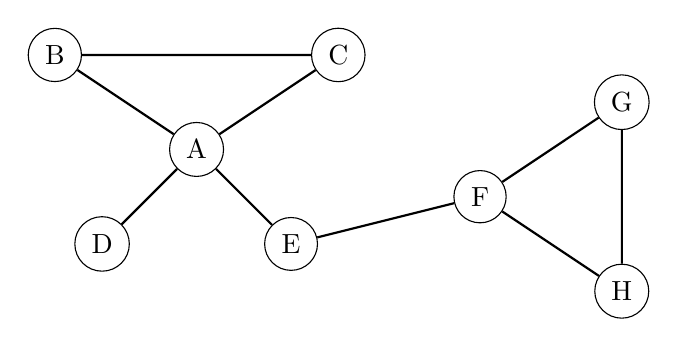
\begin{tikzpicture}[scale=1.2]
    % 左边星形+三角
    \node[draw, circle] (A) at (0, 1) {A};
    \node[draw, circle] (B) at (-1.5, 2) {B};
    \node[draw, circle] (C) at (1.5, 2) {C};
    \node[draw, circle] (D) at (-1, 0) {D};
    \node[draw, circle] (E) at (1, 0) {E};
    
    % 右边三角形
    \node[draw, circle] (F) at (3, 0.5) {F};
    \node[draw, circle] (G) at (4.5, 1.5) {G};
    \node[draw, circle] (H) at (4.5, -0.5) {H};
    
    % 星形的边
    \draw[thick] (A) -- (B);
    \draw[thick] (A) -- (C);
    \draw[thick] (A) -- (D);
    \draw[thick] (A) -- (E);
    \draw[thick] (B) -- (C);
    
    % 连接边（使图连通）
    \draw[thick] (E) -- (F);
    
    % 三角形的边
    \draw[thick] (F) -- (G);
    \draw[thick] (G) -- (H);
    \draw[thick] (F) -- (H);
\end{tikzpicture}
\end{center}

\textbf{9条边}：(A,B), (A,C), (A,D), (A,E), (B,C), (E,F), (F,G), (G,H), (F,H)

\textbf{结构}：星形（A为中心）+ 三角形（F,G,H）+ 连接边(E,F)

\textbf{这是一个连通图}：可以从任意顶点走到任意其他顶点

\end{blackboard}

\begin{blackboard}[方法0：暴力枚举（精确最优）]

\textbf{枚举所有可能的顶点子集}：$2^8 = 256$ 种

\textbf{分析最优解}：

\textbf{星形部分}：A连接4条边，选A可以覆盖(A,B), (A,C), (A,D), (A,E)

但还剩边(B,C)，需要B或C至少选一个

$\Rightarrow$ 星形部分最少需要\textbf{2个}顶点

\textbf{连接部分}：边(E,F)需要E或F至少选一个

\textbf{三角形部分}：3条边，每个顶点覆盖2条

$\Rightarrow$ 三角形最少需要\textbf{2个}顶点

\textbf{最优解}：选 $\{A, B, F, G\}$ 或 $\{A, C, F, G\}$ 等，\textbf{OPT = 4}

验证 $\{A, B, F, G\}$：覆盖所有9条边 \checkmark

\textbf{计算量}：$O(2^n \cdot m)$，$n=8$ 时 256次检查，$n=100$ 时 $10^{30}$ 次！

\end{blackboard}

\begin{blackboard}[方法1：贪心算法（选度数最大的顶点）]

\textbf{贪心策略}：每次选\textbf{覆盖最多未覆盖边}的顶点

\textbf{初始}：未覆盖边 = 全部9条

\textbf{各顶点度数}：A:4, B:2, C:2, D:1, E:2, F:3, G:2, H:2

\textbf{Round 1}：选 A（度数4），覆盖 (A,B), (A,C), (A,D), (A,E)

剩余未覆盖：(B,C), (E,F), (F,G), (G,H), (F,H)

\textbf{Round 2}：F覆盖3条 (E,F), (F,G), (F,H)，选 F

剩余未覆盖：(B,C), (G,H)

\textbf{Round 3}：B或C覆盖1条，G或H覆盖1条

选 B，剩余：(G,H)

\textbf{Round 4}：选 G

\textbf{贪心解}：$\{A, F, B, G\}$，\textbf{成本 = 4}

\textbf{这次恰好等于最优}！但贪心不总是最优...

\end{blackboard}

\begin{blackboard}[贪心算法的问题]

\textbf{贪心的近似比}：$O(\log n)$，不是常数！

\textbf{为什么贪心可能差？}

贪心每次选``当前最好''，但可能错过``全局更优''的组合

\end{blackboard}

\begin{blackboard}[贪心差的例子：双梯形图]

\begin{center}
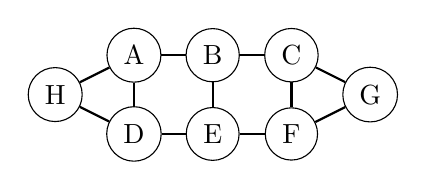
\begin{tikzpicture}[scale=1.0]
    \node[draw, circle] (A) at (0, 1) {A};
    \node[draw, circle] (B) at (1, 1) {B};
    \node[draw, circle] (C) at (2, 1) {C};
    \node[draw, circle] (D) at (0, 0) {D};
    \node[draw, circle] (E) at (1, 0) {E};
    \node[draw, circle] (F) at (2, 0) {F};
    \node[draw, circle] (G) at (3, 0.5) {G};
    \node[draw, circle] (H) at (-1, 0.5) {H};
    
    \draw[thick] (A) -- (B);
    \draw[thick] (B) -- (C);
    \draw[thick] (D) -- (E);
    \draw[thick] (E) -- (F);
    \draw[thick] (A) -- (D);
    \draw[thick] (B) -- (E);
    \draw[thick] (C) -- (F);
    \draw[thick] (C) -- (G);
    \draw[thick] (F) -- (G);
    \draw[thick] (A) -- (H);
    \draw[thick] (D) -- (H);
\end{tikzpicture}
\end{center}

\textbf{11条边}，度数：B:3, E:3, C:3, F:3, A:3, D:3, G:2, H:2

\textbf{贪心}（度数都是3时可能选错）：

假设选 B $\to$ 剩余8条边 $\to$ 选 E $\to$ 剩余5条边 $\to$ 选 C $\to$ 剩余2条边 $\to$ 选 H

\textbf{贪心解}：$\{B, E, C, H\}$，\textbf{成本 = 4}

\textbf{最优解}：$\{A, F, G\}$ 或 $\{D, C, H\}$？让我们检验：

$\{B, E, G, H\}$：覆盖所有11条边，\textbf{成本 = 4}

\textbf{能否成本3？}尝试 $\{B, F, H\}$：

B覆盖(A,B), (B,C), (B,E) \checkmark

F覆盖(E,F), (C,F), (F,G) \checkmark

H覆盖(A,H), (D,H) \checkmark

剩余：(D,E), (A,D), (C,G) 未覆盖！\textbf{成本3不够}

\textbf{结论}：这个例子最优是4，贪心也是4——\textbf{贪心运气好}

\end{blackboard}

\begin{blackboard}[贪心真正差的例子：层次覆盖]

\textbf{构造}（$n$个元素）：

层1：1个集合覆盖全部$n$个，成本 = $\log n$

层2：2个集合各覆盖$n/2$个，每个成本 = $\log n - 1$

层3：4个集合各覆盖$n/4$个，每个成本 = $\log n - 2$

...

层$\log n$：$n$个集合各覆盖1个，每个成本 = 1

\textbf{性价比}：每层都是 $\frac{\text{覆盖数}}{\text{成本}} = \frac{n/2^{k-1}}{\log n - k + 1}$

\textbf{关键}：底层集合的性价比更高！

\textbf{贪心}：从底层开始选，需要选 $\Theta(n)$ 个集合

\textbf{最优}：选顶层1个集合，成本 = $\log n$

\textbf{近似比}：$\frac{n}{\log n} = \Theta\left(\frac{n}{\log n}\right)$

\textbf{实际上}：贪心的严格近似比是 $H_n \approx \ln n$（调和级数）

\end{blackboard}

\begin{blackboard}[具体数值：顶点覆盖的 LP 与阈值舍入]

\textbf{图}：6 个顶点，3 条互不相交的边（一个完美匹配）

$$1 - 2 \qquad 3 - 4 \qquad 5 - 6$$

\textbf{顶点覆盖的 LP 松弛}：

$$
\min \sum_{v=1}^6 x_v
$$

满足

$$
x_1 + x_2 \ge 1,\qquad
x_3 + x_4 \ge 1,\qquad
x_5 + x_6 \ge 1,
$$

以及

$$
0 \le x_v \le 1 \qquad (\forall v).
$$

\textbf{LP 最优值}：

由于三条边彼此独立，问题可以分解为 3 个相同的小问题：
对每一条边 $\{u,v\}$，都要解

$$
\min x_u + x_v
\quad \text{s.t.}\quad
x_u + x_v \ge 1,\quad 0 \le x_u,x_v \le 1.
$$

这个小问题的最优值显然是 $1$，因此总的 LP 最优值为

$$
\mathrm{LP}^\star = 1 + 1 + 1 = 3.
$$

例如，下面这个分数解就是一个 LP 最优解：

$$
x_1 = x_2 = x_3 = x_4 = x_5 = x_6 = 0.5.
$$

\textbf{整数最优解}：

对于每条边，至少要选一个端点，因此整数最优解也恰好是每条边选一个点，例如

$$
\{1,3,5\},
\qquad
\mathrm{ILP}^\star = 3.
$$

所以在这个例子中，

$$
\mathrm{LP}^\star = \mathrm{ILP}^\star = 3.
$$

\textbf{注意}：这里\emph{没有整数间隙}，但这并不意味着所有 LP 最优解都是整数解；
上面的全 $0.5$ 解仍然是一个最优的分数解。

\textbf{阈值舍入}（选择所有满足 $x_v \ge 0.5$ 的顶点）：

由于上面的分数最优解满足

$$
x_v = 0.5 \qquad (\forall v),
$$

所以按阈值规则，6 个顶点会被\emph{全部选入}。于是舍入后的顶点覆盖大小为

$$
|S| = 6.
$$

而真正的最优整数解大小只有

$$
\mathrm{OPT} = 3.
$$

因此该舍入解与最优解的比值为

$$
\frac{6}{3} = 2.
$$

\textbf{结论}：

这个例子说明：
\begin{itemize}
    \item LP 本身在这里是精确的：$\mathrm{LP}^\star = \mathrm{ILP}^\star$；
    \item 但是简单的阈值舍入 $x_v \ge 0.5 \Rightarrow 1$ 仍可能把代价放大到 2 倍；
    \item 因而，顶点覆盖的 $2$-近似紧性可以来自\textbf{舍入步骤}，而不一定来自 LP 与 ILP 之间的整数间隙。
\end{itemize}

把这个例子推广到任意 $n/2$ 条独立边时，结论完全一样：
LP 最优值始终为 $n/2$，而阈值舍入会选出全部 $n$ 个顶点，因此比值始终达到 $2$。

\end{blackboard}

\begin{blackboard}[贪心 vs LP舍入：关键区别]

\textbf{贪心}：
\begin{itemize}
    \item 优点：简单快速，$O(nm)$
    \item 缺点：只看局部，近似比 $O(\log n)$
    \item 无理论保证！
\end{itemize}

\textbf{LP舍入}：
\begin{itemize}
    \item 优点：考虑全局约束，近似比是\textbf{常数}（Vertex Cover是2）
    \item 缺点：需要求解LP，$O(n^{2.5})$
    \item \textbf{有严格理论保证}！
\end{itemize}

\textbf{实践中}：

小规模（$n < 100$）：两者差不多，贪心更快

大规模（$n > 10^4$）：LP舍入更可靠

\textbf{为什么LP舍入更好？}

LP``看到''了所有约束的全局结构

贪心只看当前一步的局部最优

\end{blackboard}

\begin{blackboard}[方法2：匹配算法（2-近似）]

\textbf{另一种 2-近似}：基于极大匹配

\textbf{算法}：
\begin{enumerate}
    \item 找任意极大匹配 $M$（贪心：每次选一条边，删除两端点）
    \item 选择 $M$ 中所有边的端点
\end{enumerate}

\textbf{应用到我们的图}：

选边 (A,B)，删除 A, B 及其相邻边

选边 (E,F)，删除 E, F 及其相邻边

选边 (G,H)，删除 G, H 及其相邻边

\textbf{极大匹配}：$M = \{(A,B), (E,F), (G,H)\}$

\textbf{解}：选 $\{A, B, E, F, G, H\}$，\textbf{成本 = 6}

\textbf{分析}：每条匹配边至少需要1个端点覆盖，所以 $|M| \leq \text{OPT}$

选了 $2|M|$ 个顶点，所以 $\leq 2 \cdot \text{OPT}$

\textbf{计算量}：$O(m)$，非常快！

\end{blackboard}

\begin{blackboard}[方法3：LP舍入（2-近似）]

\textbf{LP 松弛}：

$\min \sum_v x_v$ \quad s.t. \quad $x_u + x_v \geq 1$ $\forall (u,v) \in E$, \quad $x_v \in [0,1]$

\textbf{求解 LP}（用单纯形法或内点法）：

$x_A = 1$（中心，值得选）

$x_B = 0.5, x_C = 0.5$（满足 $x_B + x_C \geq 1$）

$x_D = 0$（A已覆盖）

$x_E = 0.5, x_F = 0.5$（满足 $x_E + x_F \geq 1$）

$x_G = 0.5, x_H = 0.5$（三角形经典解）

\textbf{LP 最优值} = $1 + 0.5 \times 6 = \mathbf{4}$

\textbf{舍入}：$x_v \geq 0.5$ 则选

\textbf{舍入后}：选 $\{A, B, C, E, F, G, H\}$，\textbf{成本 = 7}

\textbf{计算量}：LP求解 $O(n^{2.5})$ 或更快

\end{blackboard}

\begin{blackboard}[方法比较：这个例子]

\begin{center}
\begin{tabular}{c|c|c|c}
方法 & 解 & 成本 & 计算量 \\
\hline
暴力枚举 & $\{A, B, F, G\}$ & \textbf{4}（最优） & $O(2^n m)$ \\
贪心 & $\{A, F, B, G\}$ & 4 & $O(nm)$ \\
匹配 & $\{A, B, E, F, G, H\}$ & 6 & $O(m)$ \\
LP舍入 & $\{A, B, C, E, F, G, H\}$ & 7 & $O(n^{3.5})$
\end{tabular}
\end{center}

\textbf{这个例子的观察}：

贪心恰好找到最优（运气好）

匹配得到 1.5 倍最优

LP舍入得到 1.75 倍最优

\textbf{但是}：LP舍入有\textbf{最坏情况保证} $\leq 2$，贪心没有！

\end{blackboard}

\begin{blackboard}[写成整数规划（ILP）]

\textbf{决策变量}：$x_v = \begin{cases} 1 & \text{选择顶点 } v \\ 0 & \text{不选} \end{cases}$

\textbf{目标函数}：$\min \; x_A + x_B + x_C + x_D + x_E + x_F + x_G + x_H$

\textbf{约束条件}（9条边，每条至少一个端点被选）：

$x_A + x_B \geq 1$ \quad $x_A + x_C \geq 1$ \quad $x_A + x_D \geq 1$

$x_A + x_E \geq 1$ \quad $x_B + x_C \geq 1$ \quad $x_E + x_F \geq 1$

$x_F + x_G \geq 1$ \quad $x_G + x_H \geq 1$ \quad $x_F + x_H \geq 1$

\textbf{整数约束}：所有 $x_v \in \{0, 1\}$

\textbf{Gurobi 求解}：$< 0.01$ 秒得到最优解

\end{blackboard}

\begin{blackboard}[LP 松弛的详细分析]

\textbf{LP 解}：$x^* = (1, 0.5, 0.5, 0, 0.5, 0.5, 0.5, 0.5)$

\textbf{验证所有约束}：

$(A,B)$: $1 + 0.5 = 1.5 \geq 1$ \checkmark \quad $(A,C)$: $1 + 0.5 = 1.5 \geq 1$ \checkmark

$(A,D)$: $1 + 0 = 1 \geq 1$ \checkmark \quad\quad $(A,E)$: $1 + 0.5 = 1.5 \geq 1$ \checkmark

$(B,C)$: $0.5 + 0.5 = 1 \geq 1$ \checkmark \quad $(E,F)$: $0.5 + 0.5 = 1 \geq 1$ \checkmark

$(F,G)$: $0.5 + 0.5 = 1 \geq 1$ \checkmark \quad $(G,H)$: $0.5 + 0.5 = 1 \geq 1$ \checkmark

$(F,H)$: $0.5 + 0.5 = 1 \geq 1$ \checkmark

\textbf{LP 最优值} = $1 + 0.5 \times 6 = \mathbf{4}$

\textbf{Integrality Gap}：$\frac{\text{ILP}}{\text{LP}} = \frac{4}{4} = 1$（这个例子没有gap！）

\end{blackboard}

\begin{blackboard}[确定性舍入]

\textbf{舍入规则}：如果 $x_v^* \geq 0.5$，就选择顶点 $v$

\textbf{应用到 LP 解}：

$x_A = 1 \geq 0.5$ $\Rightarrow$ 选 A \checkmark

$x_B = 0.5 \geq 0.5$ $\Rightarrow$ 选 B \checkmark

$x_C = 0.5 \geq 0.5$ $\Rightarrow$ 选 C \checkmark

$x_D = 0 < 0.5$ $\Rightarrow$ 不选 D

$x_E = 0.5 \geq 0.5$ $\Rightarrow$ 选 E \checkmark

$x_F = 0.5 \geq 0.5$ $\Rightarrow$ 选 F \checkmark

$x_G = 0.5 \geq 0.5$ $\Rightarrow$ 选 G \checkmark

$x_H = 0.5 \geq 0.5$ $\Rightarrow$ 选 H \checkmark

\textbf{舍入后的解}：选 \{A, B, C, E, F, G, H\}，共 \textbf{7} 个顶点

\end{blackboard}

\begin{blackboard}[分析近似比]

\textbf{这个例子的结果}：

ILP 最优 = 4

LP 最优 = 4

舍入后 = 7

\textbf{近似比} = $\frac{7}{4} = 1.75 < 2$ \checkmark

\textbf{为什么舍入后选了 7 个而不是 4 个？}

因为 LP 解中有 6 个变量 $= 0.5$，舍入规则把它们都选了

但最优解只需要从每对``互补''的顶点中选一个

\textbf{例如}：边(B,C)只需要选B或C，不需要都选

\textbf{这是确定性舍入的局限}：无法区分``都是 0.5''的情况

\end{blackboard}

\begin{blackboard}[2-近似的证明]

\textbf{定理}：确定性舍入是 Vertex Cover 的 2-近似算法

\textbf{证明}：

\textbf{Step 1：舍入后的解一定可行}

对于任意边 $(u, v)$，LP 约束保证 $x_u^* + x_v^* \geq 1$

$\Rightarrow$ 至少有一个 $\geq 0.5$（否则和 $< 1$）

$\Rightarrow$ 舍入后至少选一个端点

$\Rightarrow$ 边 $(u, v)$ 被覆盖 \checkmark

\textbf{Step 2：舍入后的值 $\leq$ 2 倍 LP}

对于每个顶点 $v$：

如果 $\hat{x}_v = 1$（选了），则 $x_v^* \geq 0.5$，所以 $\hat{x}_v \leq 2 x_v^*$

如果 $\hat{x}_v = 0$（没选），则 $\hat{x}_v = 0 \leq 2 x_v^*$

\textbf{求和}：$\sum_v \hat{x}_v \leq 2 \sum_v x_v^* = 2 \cdot \text{LP}$

\textbf{Step 3：LP $\leq$ ILP}

$\text{算法} \leq 2 \cdot \text{LP} \leq 2 \cdot \text{ILP} = 2 \cdot \text{OPT}$ \quad $\square$

\end{blackboard}

\begin{blackboard}[方法总结：Vertex Cover]

\begin{center}
\begin{tabular}{c|c|c|c}
方法 & 近似比 & 时间复杂度 & 特点 \\
\hline
暴力枚举 & 1（精确） & $O(2^n m)$ & 只能小规模 \\
贪心 & $O(\log n)$ & $O(nm)$ & 快但不稳定 \\
匹配 & 2 & $O(m)$ & 最快，保证2倍 \\
LP舍入 & 2 & $O(n^{2.5})$ & 有理论保证
\end{tabular}
\end{center}

\textbf{实践建议}：

$n < 30$：用 Gurobi/CPLEX 求精确解

$n < 10^4$：匹配算法（快速，保证2倍）

$n$ 很大：LP舍入 + GPU 并行

\textbf{理论极限}：除非 P=NP，不存在 $(2-\epsilon)$-近似算法！

\end{blackboard}

\begin{blackboard}[思考：为什么不同方法差这么多？]

\textbf{贪心}：局部最优 $\neq$ 全局最优

每步选``当前最好''，可能错过更好的整体方案

\textbf{匹配}：简单但保守

每条匹配边选两个端点，肯定覆盖，但可能多选

\textbf{LP舍入}：利用全局信息

LP 考虑了所有约束，但舍入时丢失了分数信息

\textbf{最优}：考虑所有可能性

指数级搜索，小规模可行，大规模不可行

\textbf{核心权衡}：计算时间 vs 解的质量

\end{blackboard}

%========================================
\subsection{随机化分析方法：从哈希表说起}
%========================================

\begin{blackboard}[为什么在这里讲哈希？]

\textbf{Vertex Cover 用的是确定性舍入}（$\geq 0.5$ 就选）

\textbf{但很多问题需要随机舍入}（以概率 $x^*$ 选）

\textbf{随机舍入的分析需要概率工具}

\textbf{哈希表}是理解这些工具的最简单例子：

\begin{center}
\begin{tabular}{c|c}
\textbf{哈希表} & \textbf{随机舍入} \\
\hline
随机选择哈希函数 & 随机决定选不选 \\
冲突 = 坏事件 & 约束被违反 = 坏事件 \\
分析期望冲突数 & 分析期望成本 \\
Chernoff 得高概率保证 & Chernoff 得高概率保证
\end{tabular}
\end{center}

\textbf{先在哈希上理解方法，再应用到近似算法}

\end{blackboard}

\begin{blackboard}[哈希的问题：为什么需要它？]

\textbf{场景}：存储 1000 个学号（8位数字），支持快速查找

\textbf{天真想法}：用学号当数组下标

array[20210001] 存学号 20210001

\textbf{问题}：学号最大 $10^8$，需要开 $10^8$ 大小的数组

但只有 1000 个学生，$99.999\%$ 空间浪费！

\textbf{哈希的解决方案}：压缩映射

$h(x) = x \mod 1000$

只需要大小 1000 的数组

$h(20210001) = 1$，$h(20210537) = 537$

查找只需要 1 次！

\end{blackboard}

\begin{blackboard}[哈希冲突与对手攻击]

\textbf{冲突}：不同学号可能映射到同一位置

$h(20210001) = 1$，$h(20211001) = 1$，$h(20221001) = 1$

都要存在 array[1]，查找变慢

\textbf{对手攻击}：如果对手知道 $h(x) = x \mod 1000$

故意选：1, 1001, 2001, ..., 999001（哈希值都是1）

全部冲突，查找退化到 $O(n)$

\textbf{2011年真实攻击}：构造大量冲突的HTTP参数，让服务器变慢

\textbf{根本原因}：确定性算法 $\Rightarrow$ 对手知道策略 $\Rightarrow$ 可针对攻击

\textbf{解决方案}：\textbf{随机化}

\end{blackboard}

\begin{blackboard}[随机哈希：Universal Hash Family]

\textbf{思想}：不用固定的 $h$，而是随机选一个

\textbf{Universal Hash Family}：一族函数 $\mathcal{H}$，满足

对任意 $x \neq y$：$P_{h \sim \mathcal{H}}[h(x) = h(y)] \leq \frac{1}{m}$

\textbf{具体构造}：$h_{a,b}(x) = ((ax + b) \mod p) \mod m$

随机选 $a, b$，对手不知道选了哪个！

\textbf{例子}：$m=8$，$p=17$，选 $a=3$，$b=5$

$h(7) = ((3 \times 7 + 5) \mod 17) \mod 8 = 26 \mod 17 \mod 8 = 9 \mod 8 = 1$

$h(15) = (50 \mod 17) \mod 8 = 16 \mod 8 = 0$

$h(23) = (74 \mod 17) \mod 8 = 6$

\textbf{对比}：$x \mod 8$ 会让 7, 15, 23 全冲突到位置 7

随机哈希后分散到 1, 0, 6

\end{blackboard}

\begin{blackboard}[期望分析]

\textbf{问题}：随机选 $h$ 后，查找 $x_i$ 期望比较多少次？

\textbf{定义指示变量}：$X_{ij} = \begin{cases} 1 & h(x_i) = h(x_j) \\ 0 & \text{否则} \end{cases}$

\textbf{查找时间} = $1 + \sum_{j \neq i} X_{ij}$（1 次 + 与冲突元素比较）

\textbf{关键}：$\mathbb{E}[X_{ij}] = P[h(x_i) = h(x_j)] \leq \frac{1}{m}$

\textbf{期望的线性性}（\textbf{不要求独立}！）：
\[
\mathbb{E}\left[1 + \sum_{j \neq i} X_{ij}\right] = 1 + \sum_{j \neq i} \mathbb{E}[X_{ij}] \leq 1 + \frac{n-1}{m}
\]

取 $m = n$：期望查找时间 $< 2$

\textbf{对比}：遍历 1000 次，二分 10 次，哈希期望 $< 2$ 次

\end{blackboard}

\begin{blackboard}[高概率保证：Chernoff Bound]

\textbf{问题}：期望好，但会不会运气差？

\textbf{Chernoff Bound}：$X_1, \ldots, X_n$ 独立 0-1 变量，$\mu = \mathbb{E}[\sum_i X_i]$
\[
P\left[\sum_i X_i > (1+\delta)\mu\right] \leq e^{-\frac{\delta^2 \mu}{3}}
\]

\textbf{应用}：某位置期望元素数 $\mu = 1$

$P[\text{元素数} > 10] \leq e^{-27} \approx 10^{-12}$

\textbf{Union Bound}：1000 个位置

$P[\text{存在某位置} > 10] \leq 1000 \times 10^{-12} = 10^{-9}$

\textbf{结论}：以 $> 99.9999999\%$ 概率，所有查找 $\leq 10$ 次

\end{blackboard}


\begin{blackboard}[Chernoff Bound 证明]

\textbf{定理}：$X_1, \ldots, X_n$ 独立 0-1 变量，$\mu = \mathbb{E}[\sum_i X_i]$，则对 $0 < \delta \leq 1$：
\[
P\left[\sum_i X_i > (1+\delta)\mu\right] \leq e^{-\frac{\delta^2 \mu}{3}}
\]

\end{blackboard}

\begin{blackboard}[第一步：指数放大 + Markov]

直接用 Markov 不等式太松。技巧：对任意 $t > 0$，做指数变换：
\[
P\left[\sum_i X_i > (1+\delta)\mu\right] = P\left[e^{t\sum_i X_i} > e^{t(1+\delta)\mu}\right] \leq \frac{\mathbb{E}\left[e^{t\sum_i X_i}\right]}{e^{t(1+\delta)\mu}}
\]
最后一步是对非负随机变量 $e^{t\sum X_i}$ 用 Markov 不等式。

\textbf{为什么要做指数变换？}

把加法变成乘法——独立性在乘法下可以拆开：
\[
\mathbb{E}\left[e^{t\sum_i X_i}\right] = \prod_i \mathbb{E}\left[e^{tX_i}\right]
\]

\end{blackboard}

\begin{blackboard}[第二步：控制每个因子]

$X_i$ 是 0-1 变量，设 $p_i = \mathbb{E}[X_i]$：
\[
\mathbb{E}[e^{tX_i}] = (1-p_i) \cdot 1 + p_i \cdot e^t = 1 + p_i(e^t - 1)
\]

利用 $1 + x \leq e^x$（对所有实数 $x$ 成立）：
\[
1 + p_i(e^t - 1) \leq e^{p_i(e^t - 1)}
\]

连乘：
\[
\prod_i \mathbb{E}[e^{tX_i}] \leq \prod_i e^{p_i(e^t - 1)} = e^{(e^t - 1)\sum_i p_i} = e^{(e^t - 1)\mu}
\]

代回第一步：
\[
P\left[\sum_i X_i > (1+\delta)\mu\right] \leq \frac{e^{(e^t-1)\mu}}{e^{t(1+\delta)\mu}} = e^{\left[(e^t - 1) - t(1+\delta)\right]\mu}
\]

\end{blackboard}

\begin{blackboard}[第三步：选最优的 $t$]

令 $f(t) = (e^t - 1) - t(1+\delta)$，求导：
\[
f'(t) = e^t - (1+\delta) = 0 \implies t^* = \ln(1+\delta)
\]

代入：
\begin{align*}
f(t^*) &= (e^{\ln(1+\delta)} - 1) - \ln(1+\delta) \cdot (1+\delta) \\
&= \delta - (1+\delta)\ln(1+\delta)
\end{align*}

\textbf{精确的 Chernoff Bound}：
\[
\boxed{P\left[\sum_i X_i > (1+\delta)\mu\right] \leq e^{\left[\delta - (1+\delta)\ln(1+\delta)\right]\mu}}
\]

\end{blackboard}

\begin{blackboard}[第四步：化简为常用形式]

需要证明：当 $0 < \delta \leq 1$ 时，
\[
\delta - (1+\delta)\ln(1+\delta) \leq -\frac{\delta^2}{3}
\]

即证 $(1+\delta)\ln(1+\delta) \geq \delta + \frac{\delta^2}{3}$。

Taylor 展开 $\ln(1+\delta) = \delta - \frac{\delta^2}{2} + \frac{\delta^3}{3} - \frac{\delta^4}{4} + \cdots$，所以：
\begin{align*}
(1+\delta)\ln(1+\delta) &= (1+\delta)\left(\delta - \frac{\delta^2}{2} + \frac{\delta^3}{3} - \cdots\right) \\
&= \delta + \frac{\delta^2}{2} - \frac{\delta^3}{6} + \cdots
\end{align*}

需要 $\delta + \frac{\delta^2}{2} - \frac{\delta^3}{6} + \cdots \geq \delta + \frac{\delta^2}{3}$，即 $\frac{\delta^2}{6} - \frac{\delta^3}{6} + \cdots \geq 0$。

当 $0 < \delta \leq 1$ 时，高阶项交替递减，可以逐对配对证明非负。

代入精确版本即得：
\[
\boxed{P\left[\sum_i X_i > (1+\delta)\mu\right] \leq e^{-\frac{\delta^2\mu}{3}}}
\]

\textit{注：此形式要求 $0 < \delta \leq 1$。精确版本 $e^{[\delta-(1+\delta)\ln(1+\delta)]\mu}$ 对所有 $\delta > 0$ 成立且更紧。}

\end{blackboard}

\begin{insight}[随机化分析的三板斧]

\textbf{工具1：指示随机变量}

把复杂事件分解成简单的 0-1 变量

\textbf{工具2：期望的线性性}

$\mathbb{E}[\sum X_i] = \sum \mathbb{E}[X_i]$，\textbf{不要求独立}！

\textbf{工具3：Chernoff + Union Bound}

从``期望好''到``高概率好''

\textbf{接下来}：用这三板斧分析随机舍入的近似算法

\end{insight}

%========================================
\begin{blackboard}[例2: Set Cover：具体例子]
\textbf{问题}：用最小成本的子集覆盖全集

\textbf{例子}：$U = \{1, 2, 3, 4, 5, 6\}$，4个子集

\begin{center}
\begin{tabular}{c|c|c}
子集 & 包含元素 & 成本 \\
\hline
$S_1$ & $\{1, 2, 3\}$ & 3 \\
$S_2$ & $\{2, 4, 5\}$ & 3 \\
$S_3$ & $\{3, 4, 6\}$ & 3 \\
$S_4$ & $\{1, 2, 3, 4, 5, 6\}$ & 5
\end{tabular}
\end{center}

\textbf{ILP}：
\begin{align*}
\min \quad & \sum_j c_j x_j \\
\text{s.t.} \quad & \sum_{j:\, e \in S_j} x_j \geq 1, \quad \forall\, e \in U \\
& x_j \in \{0, 1\}
\end{align*}

\textbf{ILP 最优}：选 $\{S_4\}$，成本 = \textbf{5}

\end{blackboard}

\begin{blackboard}[Set Cover：单轮随机舍入的问题]

\textbf{LP 松弛}：$x_j \in [0, 1]$，设最优解为 $x^*$，最优值 $\text{LP}^* \leq \text{OPT}$。

\textbf{朴素舍入}：以概率 $x_j^*$ 选择 $S_j$。

\textbf{期望成本}很好：$\mathbb{E}[\text{成本}] = \sum_j c_j x_j^* = \text{LP}^*$

\textbf{但覆盖性很差}。对元素 $e$，设包含 $e$ 的子集的 LP 值之和 $\geq 1$：
\[
P[e \text{ 未覆盖}] = \prod_{j:\, e\in S_j} (1 - x_j^*) \leq \prod_{j:\, e\in S_j} e^{-x_j^*} = e^{-\sum_{j:\,e\in S_j} x_j^*} \leq \frac{1}{e} \approx 0.368
\]

每个元素有约 $37\%$ 的概率没被覆盖——单轮不够！

\end{blackboard}

\begin{blackboard}[Set Cover：正确的算法]

\textbf{关键思路}：放大选择概率 + 确定性兜底。

\textbf{算法}：
\begin{enumerate}
    \item 解 LP 松弛，得最优解 $x^*$
    \item \textbf{随机步}：独立地以概率 $p_j = \min(1,\; \ln n \cdot x_j^*)$ 选择 $S_j$
    \item \textbf{兜底步}：对每个仍未覆盖的元素 $e$，选包含 $e$ 的最便宜子集 $S(e)$
\end{enumerate}

\textit{注意：选择概率是 $\ln n \cdot x_j^*$ 而不是 $x_j^*$——放大了 $\ln n$ 倍！}

\textit{算法一定输出可行解（兜底步保证），问题只是成本有多大。}

\end{blackboard}

\begin{blackboard}[Set Cover：成本分析]

总成本 = 随机步成本 + 兜底步成本。由期望的线性性：
\[
\mathbb{E}[\text{总成本}] = \mathbb{E}[\text{alg}_1] + \mathbb{E}[\text{alg}_2]
\]

\textbf{第一部分}：随机步的期望成本
\[
\mathbb{E}[\text{alg}_1] = \sum_j c_j \cdot p_j \leq \sum_j c_j \cdot \ln n \cdot x_j^* = \ln n \cdot \text{LP}^*
\]

\textbf{第二部分}：兜底步的期望成本

先证一个引理：对任意元素 $e$，包含 $e$ 的最便宜子集 $S(e)$ 的成本满足
\[
c(S(e)) \leq \text{LP}^*
\]
\textit{证明}：$\text{LP}^* = \sum_j c_j x_j^* \geq \sum_{j:\,e\in S_j} c_j x_j^* \geq c(S(e)) \cdot \underbrace{\sum_{j:\,e\in S_j} x_j^*}_{\geq 1}$

\end{blackboard}

\begin{blackboard}[Set Cover：兜底成本的控制]

设 $Y_e$ 为元素 $e$ 在随机步后仍未覆盖的指示变量。

\[
\mathbb{E}[\text{alg}_2] = \sum_{e \in U} c(S(e)) \cdot \mathbb{E}[Y_e] \leq \text{LP}^* \cdot \sum_{e \in U} \mathbb{E}[Y_e]
\]

\textbf{关键}：放大概率后，$e$ 未覆盖的概率非常小：
\[
\mathbb{E}[Y_e] = \prod_{j:\,e\in S_j}(1 - p_j) \leq \prod_{j:\,e\in S_j} e^{-\ln n \cdot x_j^*} = e^{-\ln n \cdot \sum_{j:\,e\in S_j} x_j^*} \leq e^{-\ln n} = \frac{1}{n}
\]

因此：
\[
\mathbb{E}[\text{alg}_2] \leq \text{LP}^* \cdot \sum_{e \in U} \frac{1}{n} = \text{LP}^* \cdot \frac{n}{n} = \text{LP}^*
\]

\textbf{合并}：
\[
\boxed{\mathbb{E}[\text{总成本}] \leq \ln n \cdot \text{LP}^* + \text{LP}^* = (1 + \ln n) \cdot \text{LP}^* \leq (1 + \ln n) \cdot \text{OPT}}
\]

\end{blackboard}

\begin{blackboard}[Set Cover：总结]

\textbf{定理}：上述随机舍入算法是 $(1 + \ln n)$-近似算法。
\begin{itemize}
    \item \textbf{一定可行}：兜底步保证所有元素被覆盖
    \item \textbf{期望成本} $\leq (1+\ln n) \cdot \text{OPT}$
    \item 随机步贡献 $\ln n \cdot \text{LP}^*$（放大概率的代价）
    \item 兜底步贡献 $\leq \text{LP}^*$（因为未覆盖概率 $\leq 1/n$，很小）
\end{itemize}

\textbf{注}：这个 $O(\log n)$ 近似比是\textbf{紧}的——除非 P = NP，Set Cover 不存在 $(1-\varepsilon)\ln n$ 近似算法（Dinur \& Steurer, 2014）。

\end{blackboard}

\begin{blackboard}[回到具体例子]

$n = 6$，$\ln 6 \approx 1.79$。LP 最优解 $x^* = (0.6, 0.5, 0.4, 0)$，$\text{LP}^* = 4.5$。

\textbf{放大后的选择概率}：$p_j = \min(1, \ln 6 \cdot x_j^*)$
\begin{center}
\begin{tabular}{c|c|c}
子集 & $x_j^*$ & $p_j = \min(1, 1.79 \cdot x_j^*)$ \\
\hline
$S_1$ & 0.6 & $\min(1, 1.07) = \mathbf{1.0}$ \\
$S_2$ & 0.5 & $\min(1, 0.90) = 0.90$ \\
$S_3$ & 0.4 & $\min(1, 0.72) = 0.72$ \\
$S_4$ & 0 & $0$
\end{tabular}
\end{center}

$S_1$ 必选（$p_1 = 1$），这就覆盖了元素 1, 2, 3。

剩余未覆盖概率：
\begin{center}
\begin{tabular}{c|c}
元素 & 未覆盖概率 \\
\hline
4 ($\in S_2, S_3$) & $(1-0.90)(1-0.72) = 0.028$ \\
5 ($\in S_2$) & $1-0.90 = 0.10$ \\
6 ($\in S_3$) & $1-0.72 = 0.28$
\end{tabular}
\end{center}

都远小于朴素舍入时的概率，兜底步几乎不需要额外花钱。

\end{blackboard}

%========================================
\subsection{例3：Max-SAT（3/4-近似）}
%========================================

\begin{blackboard}[什么是 Max-SAT 问题？]

\textbf{SAT 问题回顾}：

给定一个布尔公式，判断是否存在一个变量赋值使公式为真。

\textbf{Max-SAT 问题}：

给定一个布尔公式（由多个子句组成），找一个变量赋值，使得\textbf{满足的子句数最多}。

\textbf{例子}：3个变量 $x_1, x_2, x_3$，4个子句

\begin{align*}
C_1 &= (x_1 \vee x_2) \quad \text{（$x_1$ 为真 或 $x_2$ 为真）} \\
C_2 &= (\bar{x}_1 \vee x_3) \quad \text{（$x_1$ 为假 或 $x_3$ 为真）} \\
C_3 &= (x_2 \vee \bar{x}_3) \quad \text{（$x_2$ 为真 或 $x_3$ 为假）} \\
C_4 &= (\bar{x}_2) \quad \text{（$x_2$ 为假）}
\end{align*}

\textbf{注意}：$\bar{x}$ 表示 $x$ 的否定（$x$ 为真时 $\bar{x}$ 为假，反之亦然）

\textbf{目标}：找一个赋值，让尽可能多的子句为真。

\end{blackboard}

\begin{blackboard}[枚举所有可能的赋值]

3个变量，每个可以是 True 或 False，共有 $2^3 = 8$ 种可能的赋值。

\textbf{赋值1}：$x_1 = T, x_2 = T, x_3 = T$

$C_1 = T \vee T = T$ \checkmark \quad
$C_2 = F \vee T = T$ \checkmark \quad
$C_3 = T \vee F = T$ \checkmark \quad
$C_4 = F$ $\times$

满足 \textbf{3} 个子句。

\textbf{赋值2}：$x_1 = T, x_2 = F, x_3 = T$

$C_1 = T \vee F = T$ \checkmark \quad
$C_2 = F \vee T = T$ \checkmark \quad
$C_3 = F \vee F = F$ $\times$ \quad
$C_4 = T$ \checkmark

满足 \textbf{3} 个子句。

\textbf{赋值3}：$x_1 = F, x_2 = T, x_3 = F$

$C_1 = F \vee T = T$ \checkmark \quad
$C_2 = T \vee F = T$ \checkmark \quad
$C_3 = T \vee T = T$ \checkmark \quad
$C_4 = F$ $\times$

满足 \textbf{3} 个子句。

\textbf{赋值4}：$x_1 = F, x_2 = F, x_3 = F$

$C_1 = F \vee F = F$ $\times$ \quad
$C_2 = T \vee F = T$ \checkmark \quad
$C_3 = F \vee T = T$ \checkmark \quad
$C_4 = T$ \checkmark

满足 \textbf{3} 个子句。

\textbf{观察}：无论怎么赋值，最多只能满足3个子句（\textbf{OPT = 3}）。

\textbf{原因}：$C_1 = (x_1 \vee x_2)$ 和 $C_4 = (\bar{x}_2)$ 存在结构性冲突——
$x_2 = T$ 则 $C_4$ 不满足；$x_2 = F$ 则要满足 $C_1$ 就需要 $x_1 = T$，这又压缩了 $C_2$ 的空间。

\end{blackboard}

\begin{blackboard}[方法1：纯随机算法（不用 LP！）]

\textbf{算法}：对每个变量，独立地以 50\% 概率设为 True，50\% 概率设为 False。

\textbf{分析子句 $C_1 = (x_1 \vee x_2)$ 被满足的概率}：

$C_1$ 不满足 $\Leftrightarrow$ $x_1 = F$ 且 $x_2 = F$

$P[C_1 \text{ 不满足}] = 0.5 \times 0.5 = 0.25$，故 $P[C_1 \text{ 满足}] = 1 - 0.25 = \mathbf{0.75}$

\textbf{一般规律}：含 $k$ 个文字的子句

$P[\text{满足}] = 1 - \frac{1}{2^k}$

\begin{center}
\begin{tabular}{c|c}
子句大小 $k$ & 满足概率 \\
\hline
1 & $1 - \frac{1}{2} = 0.5$ \\
2 & $1 - \frac{1}{4} = 0.75$ \\
3 & $1 - \frac{1}{8} = 0.875$ \\
$\infty$ & $\to 1$
\end{tabular}
\end{center}

\textbf{特点}：$k$ 越大概率越高——纯随机对\textbf{长子句}很好，但对\textbf{短子句}差（$k=1$ 时仅 $0.5$）。

\end{blackboard}

\begin{blackboard}[计算我们例子的期望]

\textbf{四个子句的满足概率}：

$C_1 = (x_1 \vee x_2)$：$k=2$，$P = 0.75$

$C_2 = (\bar{x}_1 \vee x_3)$：$k=2$，$P = 0.75$

$C_3 = (x_2 \vee \bar{x}_3)$：$k=2$，$P = 0.75$

$C_4 = (\bar{x}_2)$：$k=1$，$P = 0.5$

\textbf{期望满足的子句数}（期望的线性性）：

$\mathbb{E}[\text{满足数}] = 0.75 + 0.75 + 0.75 + 0.5 = \mathbf{2.75}$

\textbf{近似比} = $\frac{2.75}{3} \approx 0.917$

\textbf{一般保证}：每个子句至少有1个文字，满足概率 $\geq 0.5$

$\Rightarrow$ 期望满足数 $\geq \frac{1}{2} \times$ 子句总数 $\geq \frac{1}{2} \times \text{OPT}$

\textbf{纯随机是 $\frac{1}{2}$-近似算法}！

\end{blackboard}

\begin{blackboard}[方法2：LP 随机舍入]

\textbf{LP 松弛}：

对每个变量 $x_i$，定义 $y_i \in [0, 1]$（$x_i$ 为真的"程度"）

对每个子句 $C_j$，定义 $z_j \in [0, 1]$（$C_j$ 被满足的"程度"）

\textbf{约束}（以 $C_2 = (\bar{x}_1 \vee x_3)$ 为例）：

$z_2 \leq (1 - y_1) + y_3$

（$C_2$ 被满足需要 $\bar{x}_1$ 或 $x_3$ 为真，$\bar{x}_1$ 为真的程度是 $1 - y_1$）

\textbf{完整 LP}：
\begin{align*}
\max \quad & z_1 + z_2 + z_3 + z_4 \\
\text{s.t.} \quad & z_1 \leq y_1 + y_2 \\
& z_2 \leq (1-y_1) + y_3 \\
& z_3 \leq y_2 + (1-y_3) \\
& z_4 \leq (1-y_2) \\
& 0 \leq z_j \leq 1, \quad 0 \leq y_i \leq 1
\end{align*}

\textbf{随机舍入}：解LP得 $(y^*, z^*)$，以概率 $y_i^*$ 令 $x_i = \text{True}$。

\end{blackboard}

\begin{blackboard}[LP 舍入的近似保证]

\textbf{定理}：对含 $k$ 个文字的子句 $C_j$，LP舍入的满足概率 $\geq (1 - (1-\frac{1}{k})^k) \cdot z_j^*$。

\textbf{证明思路}：设子句 $C_j$ 含 $k$ 个文字，LP解中各文字为真的程度之和 $\geq z_j^*$。由 AM-GM 不等式，不满足的概率：
\[
\prod_{i=1}^{k}(1-p_i) \leq \left(\frac{\sum(1-p_i)}{k}\right)^k = \left(1 - \frac{\sum p_i}{k}\right)^k \leq \left(1 - \frac{z_j^*}{k}\right)^k
\]

满足概率 $\geq 1 - (1 - z_j^*/k)^k \geq (1-(1-1/k)^k) \cdot z_j^*$（因为 $z_j^* \leq 1$）。

\begin{center}
\begin{tabular}{c|c}
子句大小 $k$ & LP舍入保证 $\geq \alpha_k \cdot z_j^*$ \\
\hline
1 & $1.0 \cdot z_j^*$ \\
2 & $0.75 \cdot z_j^*$ \\
3 & $\approx 0.704 \cdot z_j^*$ \\
$\infty$ & $\to (1-1/e) \cdot z_j^* \approx 0.632 \cdot z_j^*$
\end{tabular}
\end{center}

\textbf{特点}：LP舍入对\textbf{短子句}很好（$k=1$ 时系数为 $1.0$），但对\textbf{长子句}退化到 $1-1/e$。

\textit{直觉：短子句文字少，LP解给出的方向很精确，舍入几乎不丢信息；长子句文字多，LP的"部分赋值"优势被稀释。}

\end{blackboard}

\begin{blackboard}[组合两种方法：3/4 近似]

\textbf{关键观察}——两种方法互补：

方法1（纯随机）对\textbf{长}子句好：$k$ 越大，$1 - 1/2^k \to 1$

方法2（LP舍入）对\textbf{短}子句好：$k=1$ 时系数 $1.0$，几乎完美

\textbf{组合方法}：两套都跑一遍取最好的那一个 

\textbf{组合后的满足概率}（利用 $z_j^* \leq 1$，且 OPT $\leq \sum z_j^*$）：

\begin{center}
\begin{tabular}{c|cc|c}
$k$ & 方法1：$1-1/2^k$ & 方法2：$\alpha_k \cdot z_j^*$ & 组合（取 $z_j^*=1$） \\
\hline
1 & $0.500$ & $1.000$ & $\frac{0.500 + 1.000}{2} = \mathbf{0.750}$ \\
2 & $0.750$ & $0.750$ & $\frac{0.750 + 0.750}{2} = \mathbf{0.750}$ \\
3 & $0.875$ & $0.704$ & $\frac{0.875 + 0.704}{2} \approx 0.790$ \\
$\infty$ & $\to 1$ & $\to 0.632$ & $\to 0.816$
\end{tabular}
\end{center}

\textbf{关键}：无论 $k$ 是多少，组合后的概率都 $\geq 0.75$！

更严格地，可以证明对任意 $k$：
\[
\frac{1}{2}\left(1 - \frac{1}{2^k}\right) + \frac{1}{2}\left(1 - \left(1 - \frac{1}{k}\right)^k\right) \geq \frac{3}{4}
\]

\textbf{结论}：组合方法是 \textbf{3/4-近似算法}！

\end{blackboard}

%========================================
\subsection{例4：Max-Cut（0.878-近似）}
%========================================

\begin{blackboard}[什么是 Max-Cut 问题？]

\textbf{问题描述}：

给定一个图，要把所有顶点分成两组 $S$ 和 $\bar{S}$。

一条边叫做``被切''的，如果它的两个端点分别在 $S$ 和 $\bar{S}$ 中。

\textbf{目标}：找一种分组方式，使被切的边数最多。

\textbf{为什么叫``Cut''？}

想象用一把刀沿着 $S$ 和 $\bar{S}$ 的边界切下去，会切断多少条边？

\textbf{例子}：考虑一个有4个顶点、5条边的图

\begin{center}
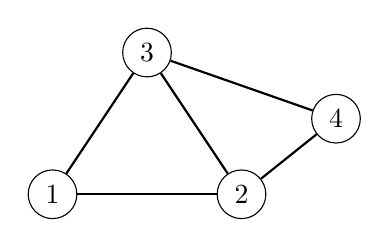
\begin{tikzpicture}[scale=1.2]
    \node[draw, circle] (1) at (0, 0) {1};
    \node[draw, circle] (2) at (2, 0) {2};
    \node[draw, circle] (3) at (1, 1.5) {3};
    \node[draw, circle] (4) at (3, 0.8) {4};
    
    \draw[thick] (1) -- (2);
    \draw[thick] (2) -- (3);
    \draw[thick] (1) -- (3);
    \draw[thick] (2) -- (4);
    \draw[thick] (3) -- (4);
\end{tikzpicture}
\end{center}

5条边分别是：(1,2), (1,3), (2,3), (2,4), (3,4)

\end{blackboard}

\begin{blackboard}[枚举一些分组方案]

\textbf{方案1}：$S = \{1\}$，$\bar{S} = \{2, 3, 4\}$

哪些边被切？一条边被切当且仅当一个端点在 $S$，另一个在 $\bar{S}$。

边 (1,2)：1在$S$，2在$\bar{S}$ $\Rightarrow$ \textbf{被切} \checkmark

边 (1,3)：1在$S$，3在$\bar{S}$ $\Rightarrow$ \textbf{被切} \checkmark

边 (2,3)：2和3都在$\bar{S}$ $\Rightarrow$ 不被切

边 (2,4)：2和4都在$\bar{S}$ $\Rightarrow$ 不被切

边 (3,4)：3和4都在$\bar{S}$ $\Rightarrow$ 不被切

\textbf{被切的边数} = \textbf{2}

\textbf{方案2}：$S = \{1, 3\}$，$\bar{S} = \{2, 4\}$

边 (1,2)：1在$S$，2在$\bar{S}$ $\Rightarrow$ \textbf{被切} \checkmark

边 (1,3)：1和3都在$S$ $\Rightarrow$ 不被切

边 (2,3)：2在$\bar{S}$，3在$S$ $\Rightarrow$ \textbf{被切} \checkmark

边 (2,4)：2和4都在$\bar{S}$ $\Rightarrow$ 不被切

边 (3,4)：3在$S$，4在$\bar{S}$ $\Rightarrow$ \textbf{被切} \checkmark

\textbf{被切的边数} = \textbf{3}

\end{blackboard}

\begin{blackboard}[继续枚举]

\textbf{方案3}：$S = \{1, 4\}$，$\bar{S} = \{2, 3\}$

边 (1,2)：被切 \checkmark

边 (1,3)：被切 \checkmark

边 (2,3)：不被切

边 (2,4)：被切 \checkmark

边 (3,4)：被切 \checkmark

\textbf{被切的边数} = \textbf{4}

\textbf{方案4}：$S = \{2, 3\}$，$\bar{S} = \{1, 4\}$

（和方案3一样，只是 $S$ 和 $\bar{S}$ 互换）

被切的边数 = \textbf{4}

\textbf{OPT = 4}（最多能切4条边，剩下的边 (2,3) 无论怎样都切不到）

\textbf{为什么}？因为顶点2和3之间有边，它们必须在同一组才能不被切，

但如果它们在同一组，(2,3) 这条边就切不到。

最优分组把 $\{2, 3\}$ 放在一起，其他4条边都被切了。

\end{blackboard}

\begin{blackboard}[为什么 LP 松弛不好用？]

\textbf{尝试用 LP}：

用 $x_v \in \{-1, +1\}$ 表示顶点 $v$ 在哪一组（+1 表示在 $S$，-1 表示在 $\bar{S}$）

边 $(u, v)$ 被切 $\Leftrightarrow$ $x_u \neq x_v$ $\Leftrightarrow$ $x_u \cdot x_v = -1$

边 $(u, v)$ 被切的``程度''可以写成：$\frac{1 - x_u x_v}{2}$

（当 $x_u x_v = -1$ 时，这个值是1；当 $x_u x_v = +1$ 时，这个值是0）

\textbf{目标函数}：$\max \sum_{(u,v) \in E} \frac{1 - x_u x_v}{2}$

\textbf{问题}：$x_u x_v$ 是\textbf{二次}的，不是线性的！

这不是 LP（线性规划），而是 QP（二次规划）。

\textbf{简单的松弛}：把 $x_v \in \{-1, +1\}$ 松弛为 $x_v \in [-1, +1]$

如果令所有 $x_v = 0$，每条边贡献 $\frac{1 - 0}{2} = 0.5$

总共 $5 \times 0.5 = 2.5$，但 OPT = 4，这个上界太松了！

\textbf{结论}：简单的 LP 松弛对 Max-Cut 不好用，我们需要更强的工具。

\end{blackboard}

\begin{blackboard}[SDP（半定规划）松弛]

\textbf{关键思想}：$x_v \in \{-1, +1\}$ 可以看成\textbf{一维单位向量}

把 -1 看成向量 $(-1)$，+1 看成向量 $(+1)$。

\textbf{推广到高维}：用 $n$ 维单位向量 $\mathbf{v}_v$ 代替标量 $x_v$

约束：$\|\mathbf{v}_v\| = 1$（向量长度为1）

两个向量的``相似程度''用\textbf{点积}衡量：$\mathbf{v}_u \cdot \mathbf{v}_v = \cos\theta$

其中 $\theta$ 是两个向量的夹角。

\textbf{SDP 目标函数}：

$\max \sum_{(u,v) \in E} \frac{1 - \mathbf{v}_u \cdot \mathbf{v}_v}{2}$

\textbf{当两个向量夹角大时}（接近相反方向），$\cos\theta$ 接近 -1，贡献接近 1。

\textbf{当两个向量夹角小时}（接近同方向），$\cos\theta$ 接近 +1，贡献接近 0。

\textbf{好消息}：SDP 可以在多项式时间内求解！（用椭球法或内点法）

\end{blackboard}

\begin{blackboard}[Goemans-Williamson 算法（1995年）]

\textbf{步骤1}：求解 SDP，得到每个顶点对应的单位向量 $\mathbf{v}_1, \mathbf{v}_2, \ldots, \mathbf{v}_n$

\textbf{步骤2}：随机选一个过原点的\textbf{超平面}

具体做法：随机选一个方向 $\mathbf{r}$（在单位球面上均匀随机）

超平面就是所有与 $\mathbf{r}$ 垂直的点构成的平面

\textbf{步骤3}：根据向量在超平面的哪一侧来分组

$S = \{\text{顶点 } v : \mathbf{v}_v \cdot \mathbf{r} > 0\}$（向量和 $\mathbf{r}$ 同侧）

$\bar{S} = \{\text{顶点 } v : \mathbf{v}_v \cdot \mathbf{r} \leq 0\}$（向量和 $\mathbf{r}$ 异侧）

\textbf{直觉}：如果两个向量 $\mathbf{v}_u$ 和 $\mathbf{v}_v$ 夹角大（接近相反），

它们很可能被超平面分到不同侧，边 $(u,v)$ 就会被切。

\end{blackboard}

\begin{blackboard}[分析：边被切的概率]

\textbf{关键问题}：边 $(u, v)$ 被切的概率是多少？

\textbf{答案}：$P[(u,v) \text{ 被切}] = \frac{\theta_{uv}}{\pi}$

其中 $\theta_{uv}$ 是向量 $\mathbf{v}_u$ 和 $\mathbf{v}_v$ 的夹角。

\textbf{为什么？}

想象在二维平面上，$\mathbf{v}_u$ 和 $\mathbf{v}_v$ 是两个单位向量，夹角为 $\theta$。

随机选一条过原点的直线（超平面在二维就是直线）。

$u$ 和 $v$ 被分开 $\Leftrightarrow$ 直线穿过 $\mathbf{v}_u$ 和 $\mathbf{v}_v$ 之间的扇形区域

这个扇形区域占整个圆的比例是 $\frac{\theta}{\pi}$（因为直线把圆分成两半）

所以 $P[\text{被分开}] = \frac{\theta}{\pi}$

\textbf{例子}：如果 $\theta = 90° = \frac{\pi}{2}$，则 $P = \frac{\pi/2}{\pi} = 0.5$

如果 $\theta = 180° = \pi$（完全相反），则 $P = 1$

如果 $\theta = 0°$（完全相同），则 $P = 0$

\end{blackboard}

\begin{blackboard}[0.878 近似比的来源]

\textbf{期望被切的边数}：

$\mathbb{E}[\text{CUT}] = \sum_{(u,v) \in E} P[(u,v) \text{ 被切}] = \sum_{(u,v) \in E} \frac{\theta_{uv}}{\pi}$

\textbf{SDP 的目标值}：

$\text{SDP} = \sum_{(u,v) \in E} \frac{1 - \cos\theta_{uv}}{2}$

\textbf{我们需要比较} $\frac{\theta}{\pi}$ 和 $\frac{1 - \cos\theta}{2}$

\textbf{数值计算}：

\begin{center}
\begin{tabular}{c|c|c|c}
$\theta$（度） & $\theta/\pi$ & $(1-\cos\theta)/2$ & 比值 \\
\hline
$60°$ & $1/3 = 0.333$ & $(1-0.5)/2 = 0.25$ & $0.333/0.25 = 1.33$ \\
$90°$ & $1/2 = 0.5$ & $(1-0)/2 = 0.5$ & $0.5/0.5 = 1.0$ \\
$120°$ & $2/3 = 0.667$ & $(1-(-0.5))/2 = 0.75$ & $0.667/0.75 = 0.89$ \\
$134°$ & $0.744$ & $0.845$ & $0.744/0.845 = \mathbf{0.878}$ \\
$180°$ & $1$ & $1$ & $1.0$
\end{tabular}
\end{center}

\textbf{最小比值}出现在 $\theta \approx 134°$，值约为 \textbf{0.878}

\textbf{结论}：$\mathbb{E}[\text{CUT}] \geq 0.878 \times \text{SDP} \geq 0.878 \times \text{OPT}$

\textbf{这是一个 0.878-近似算法！}

\end{blackboard}

%========================================
\subsection{例5：Scheduling（2-近似）}
%========================================

\begin{blackboard}[无关机器调度问题]

\textbf{问题}：
\begin{itemize}
    \item $n$ 个作业，$m$ 台机器
    \item 作业 $j$ 在机器 $i$ 上需时间 $p_{ij}$（无关机器）
    \item 目标：最小化 makespan（最后完成时间）
\end{itemize}

\textbf{具体例子}：3个作业，2台机器

\begin{center}
\begin{tabular}{c|c|c}
& 机器A & 机器B \\
\hline
作业1 & 3 & 5 \\
作业2 & 4 & 2 \\
作业3 & 2 & 4
\end{tabular}
\end{center}

\textbf{目标}：安排作业，使最后完成时间最短

\end{blackboard}

\begin{blackboard}[调度问题：枚举方案]

\textbf{方案1}：全给机器A

机器A负载 = $3 + 4 + 2 = 9$，机器B负载 = 0

Makespan = $\max(9, 0) = \mathbf{9}$

\textbf{方案2}：作业1给A，作业2,3给B

机器A负载 = 3，机器B负载 = $2 + 4 = 6$

Makespan = $\max(3, 6) = \mathbf{6}$

\textbf{方案3}：作业1,3给A，作业2给B

机器A负载 = $3 + 2 = 5$，机器B负载 = 2

Makespan = $\max(5, 2) = \mathbf{5}$

\textbf{最优方案}：作业3给A（耗时2），作业1,2给B（耗时$5+2=7$）

Makespan = $\max(2, 7) = 7$？不对，让我重新算...

\textbf{方案4}：作业2给B，作业1,3给A

机器A = $3+2=5$，机器B = 2

Makespan = \textbf{5}（这是最优！）

\end{blackboard}

\begin{blackboard}[调度问题：LP松弛]

\textbf{ILP}：$x_{ij} = 1$ 表示作业 $j$ 分配给机器 $i$
\begin{align*}
\min \quad & T \\
\text{s.t.} \quad & 3x_{A1} + 4x_{A2} + 2x_{A3} \leq T \quad \text{（机器A负载）} \\
& 5x_{B1} + 2x_{B2} + 4x_{B3} \leq T \quad \text{（机器B负载）} \\
& x_{A1} + x_{B1} = 1, \; x_{A2} + x_{B2} = 1, \; x_{A3} + x_{B3} = 1
\end{align*}

\textbf{LP松弛}：允许 $x_{ij} \in [0,1]$（作业可以``分割''）

\textbf{LP解}：$x_{A1}^* = 1, x_{B2}^* = 1, x_{A3}^* = 1$

机器A负载 = $3 + 2 = 5$，机器B负载 = 2

$T^* = 5$（刚好等于ILP最优！这个例子没有Gap）

\end{blackboard}

\begin{blackboard}[调度问题：有Gap的例子]

\textbf{3个相同作业，2台机器}，处理时间全为1：

\begin{center}
\begin{tabular}{c|c|c}
& 机器A & 机器B \\
\hline
作业1 & 1 & 1 \\
作业2 & 1 & 1 \\
作业3 & 1 & 1
\end{tabular}
\end{center}

\textbf{ILP最优}：3个作业分给2台机器，鸽巢原理某台至少分到2个

Makespan $T^*_{\text{ILP}} = \mathbf{2}$

\textbf{LP松弛}：允许分割作业，每个作业各一半给两台机器
\[
x_{A,j}^* = x_{B,j}^* = 0.5, \quad j = 1,2,3
\]

每台机器负载 $= 3 \times 0.5 \times 1 = 1.5$

$T^*_{\text{LP}} = \mathbf{1.5}$

\[
\boxed{\text{Integrality Gap} = \frac{T^*_{\text{ILP}}}{T^*_{\text{LP}}} = \frac{2}{1.5} = \frac{4}{3}}
\]

\textit{LP可以把作业"切开"均匀摊给两台机器，但整数解无法均分奇数个相同作业。}

\end{blackboard}

\begin{blackboard}[Scheduling 的舍入]

\textbf{LP 解的结构}：

每个作业 $j$ 最多被``分割''到 $m$ 台机器

$\Rightarrow$ 作业-机器的分配形成一个\textbf{二分图}

\textbf{舍入方法}：

使用二分图匹配，把分数分配转为整数分配

\textbf{分析}：

每台机器最多增加一个``额外''作业

$\Rightarrow$ 负载最多翻倍

\textbf{结论}：\textbf{2-近似}

\textbf{更好的结果}：通过更复杂的舍入，可以达到 $(2 - 1/m)$-近似

\end{blackboard}

%========================================
\subsection{例6：Facility Location（3-近似）}
%========================================

\begin{blackboard}[设施选址问题]

\textbf{问题}：
\begin{itemize}
    \item $m$ 个可能的设施位置，开设成本 $f_i$
    \item $n$ 个客户，客户 $j$ 到设施 $i$ 的服务成本 $c_{ij}$
    \item 目标：最小化总成本（开设 + 服务）
\end{itemize}

\textbf{具体例子}：2个设施，3个客户

设施开设成本：$f_1 = 10$，$f_2 = 8$

服务成本：
\begin{center}
\begin{tabular}{c|c|c|c}
& 客户A & 客户B & 客户C \\
\hline
设施1 & 2 & 5 & 3 \\
设施2 & 4 & 1 & 6
\end{tabular}
\end{center}

\end{blackboard}

\begin{blackboard}[设施选址：枚举方案]

\textbf{方案1}：只开设施1

开设成本 = 10

服务成本 = $2 + 5 + 3 = 10$

总成本 = \textbf{20}

\textbf{方案2}：只开设施2

开设成本 = 8

服务成本 = $4 + 1 + 6 = 11$

总成本 = \textbf{19}

\textbf{方案3}：两个都开

开设成本 = $10 + 8 = 18$

服务成本 = $\min(2,4) + \min(5,1) + \min(3,6) = 2 + 1 + 3 = 6$

总成本 = \textbf{24}（虽然服务便宜，但开设太贵）

\textbf{最优}：方案2，总成本 = 19

\end{blackboard}

\begin{blackboard}[设施选址：LP松弛]

\textbf{ILP}：
\begin{align*}
\min \quad & 10 y_1 + 8 y_2 + 2x_{1A} + 5x_{1B} + 3x_{1C} + 4x_{2A} + x_{2B} + 6x_{2C} \\
\text{s.t.} \quad & x_{1A} + x_{2A} = 1 \quad \text{（客户A被服务）} \\
& x_{1B} + x_{2B} = 1 \quad \text{（客户B被服务）} \\
& x_{1C} + x_{2C} = 1 \quad \text{（客户C被服务）} \\
& x_{1j} \leq y_1, \; x_{2j} \leq y_2 \quad \forall j
\end{align*}

\textbf{LP解}（可能）：$y_1^* = 0.5, y_2^* = 0.5$

$x_{1A}^* = 0.5, x_{2A}^* = 0.5$（客户A各一半）

$x_{1B}^* = 0, x_{2B}^* = 1$（客户B全给设施2，便宜）

$x_{1C}^* = 0.5, x_{2C}^* = 0.5$（客户C各一半）

\textbf{LP成本}：$10 \times 0.5 + 8 \times 0.5 + ...$

\end{blackboard}

\begin{blackboard}[Facility Location 的随机舍入]

\textbf{LP 解的含义}：
\begin{itemize}
    \item $y_i^*$：设施 $i$ 的``开设程度''
    \item $x_{ij}^*$：客户 $j$ 被设施 $i$ 服务的``程度''
\end{itemize}

\textbf{随机舍入}：
\begin{enumerate}
    \item 每个客户 $j$ 按概率 $x_{ij}^*$ 选择``首选''设施 $i$
    
    例：客户A以50\%选设施1，50\%选设施2
    
    \item 开设所有被选为首选的设施
    
    例：假设客户A选了1，客户B选了2，客户C选了1
    
    $\Rightarrow$ 开设设施1和2
    
    \item 客户连接到最近的开设设施
\end{enumerate}

\textbf{分析}（Shmoys, Tardos, Aardal）：

期望成本 $\leq 3 \cdot \text{OPT}_{\text{LP}} \leq 3 \cdot \text{OPT}$

\textbf{目前最好}：1.488-近似（Li, 2013）

\end{blackboard}

%========================================
\subsection{更多例子概览}
%========================================

\begin{blackboard}[连续化近似算法大全]

\begin{center}
\begin{tabular}{c|c|c|c}
\textbf{问题} & \textbf{松弛} & \textbf{舍入方法} & \textbf{近似比} \\
\hline
Vertex Cover & LP & 确定性阈值 & 2 \\
Set Cover & LP & 随机 + 重复 & $O(\log n)$ \\
Max-SAT & LP & 随机组合 & 3/4 \\
Max-Cut & \textbf{SDP} & 随机超平面 & 0.878 \\
Scheduling & LP & 二分图匹配 & 2 \\
Facility Location & LP & 随机首选 & 3 \\
\hline
$k$-Median & LP & 随机 + 贪心 & 3.25 \\
Multiway Cut & LP & 随机球 & 1.5 \\
Sparsest Cut & \textbf{SDP} & 随机投影 & $O(\sqrt{\log n})$ \\
Graph Coloring & \textbf{SDP} & 随机向量 & $O(n^{0.25})$ \\
Correlation Clustering & LP & 随机 pivot & 3
\end{tabular}
\end{center}

\textbf{模式}：几乎所有经典组合优化都有``松弛 + 舍入''！

\end{blackboard}


%----------------------------------------
\subsection{超越期望：随机舍入的深层理论}
%----------------------------------------

\begin{blackboard}[随机化为何能超越简单松弛？]

\textbf{核心问题}：随机舍入凭什么能得到好的近似？

\textbf{答案}：三个数学工具

\textbf{工具1：期望的线性性}
\[
\mathbb{E}\left[\sum_j X_j\right] = \sum_j \mathbb{E}[X_j]
\]
即使 $X_j$ 之间\textbf{不独立}，也成立！

\textbf{工具2：初等不等式} $1 - x \leq e^{-x}$

\textbf{数值验证}：$x = 0.5$ 时，$1 - 0.5 = 0.5$，$e^{-0.5} \approx 0.607$，确实 $0.5 \leq 0.607$ \checkmark

\textbf{工具3：Union Bound}
\[
P\left[\bigcup_i A_i\right] \leq \sum_i P[A_i]
\]

\textbf{例子}：10个事件，每个发生概率0.01，则至少一个发生的概率 $\leq 0.1$

\end{blackboard}



\begin{blackboard}[Gurobi / CPLEX 内部技术]

\textbf{商业求解器的核心组件}：

\textbf{1. 预处理（Presolve）}
\begin{itemize}
    \item 变量固定：$x_i^* = 0$ 或 $1$ 时直接固定
    \item 约束传播：利用约束推导更多固定
    \item 冗余约束删除、变量聚合
\end{itemize}

\textbf{2. 割平面（Cutting Planes）}
\begin{itemize}
    \item LP 解不是整数时，添加新约束``切掉''它
    \item Gomory cuts：从 LP 单纯形表推导
    \item 问题特定割：Cover cuts, Clique cuts
\end{itemize}

\textbf{3. 分支定界 + 启发式}
\begin{itemize}
    \item 用 LP 松弛计算界
    \item Feasibility Pump, RINS 找可行解
    \item \textbf{内部也用随机舍入}！
\end{itemize}

\end{blackboard}

\begin{blackboard}[求解器 vs 近似算法]

\begin{center}
\begin{tabular}{c|c|c}
& \textbf{商业求解器} & \textbf{近似算法} \\
\hline
目标 & 精确最优 & $\alpha$-近似 \\
时间保证 & 无（可能指数级） & 多项式时间 \\
适用规模 & $10^3$-$10^6$ 变量 & 任意大 \\
GPU友好 & 通常不 & 可以设计
\end{tabular}
\end{center}

\textbf{实践建议}：

\textbf{小规模}（$< 10^4$）：Gurobi/CPLEX，几秒到几分钟

\textbf{大规模/实时}：近似算法（时间可预测）

\textbf{大量实例}：近似算法 + GPU 并行

\end{blackboard}

\begin{blackboard}[条件期望法：去随机化]

\textbf{定理}：如果随机算法期望给出 $\alpha$-近似，则存在\textbf{确定性}解

\textbf{方法}：依次确定每个变量，每步选使条件期望更好的值

\end{blackboard}

\begin{blackboard}[条件期望法：MAX-SAT 详细例子]

\textbf{回到之前的例子}：4个子句

$C_1 = x_1$，$C_2 = x_1 \lor x_2$，$C_3 = \neg x_1 \lor x_3$，$C_4 = x_1 \lor x_2 \lor x_3$

\textbf{用纯随机策略}（每个变量 1/2 概率 True）

\textbf{初始期望}：
$W() = P[C_1] + P[C_2] + P[C_3] + P[C_4]$
$= 0.5 + 0.75 + 0.75 + 0.875 = 2.875$

\textbf{Step 1：决定 $x_1$}

$W(x_1 = T)$：$C_1$ 必满足，$C_3 = \neg T \lor x_3 = x_3$

$= 1 + 1 + 0.5 + 1 = 3.5$（$C_2, C_4$ 必满足，$C_3$ 概率0.5）

$W(x_1 = F)$：$C_1$ 必不满足

$= 0 + 0.5 + 1 + 0.75 = 2.25$

\textbf{选 $x_1 = T$}（3.5 > 2.25）

\end{blackboard}


\begin{blackboard}[随机化与并行的天然契合]

\textbf{随机化的四大优势}：

\textbf{1. 打破对称性}

三角形三个顶点对称，确定性算法难以选择

随机化：各 1/2 概率选，天然打破对称

\textbf{2. 期望线性性}

$\mathbb{E}[\sum X_i] = \sum \mathbb{E}[X_i]$，不要求独立！

MAX-SAT 证明的核心

\textbf{3. 与LP完美配合}

LP解 $x^* \in [0,1]$：天然的概率

\textbf{4. 天然可并行}

100次独立舍入，GPU同时进行

取最好的，几乎免费改进！

\end{blackboard}

%========================================
\section{GPU 友好性}
%========================================

\begin{blackboard}[传统 vs 现代方法]

\begin{center}
\begin{tabular}{c|c|c}
& \textbf{传统算法} & \textbf{连续化 + 随机化} \\
\hline
典型方法 & 分支定界、DP & LP/SDP + 随机舍入 \\
\hline
计算模式 & 树搜索、顺序依赖 & 矩阵运算、独立采样 \\
\hline
并行性 & \textcolor{red}{差} & \textcolor{green!50!black}{好} \\
\hline
GPU 友好 & \textcolor{red}{否} & \textcolor{green!50!black}{是} \\
\hline
精度 & 精确 & 近似（有保证） \\
\hline
可扩展性 & $\sim 10^3$ & $\sim 10^6$
\end{tabular}
\end{center}

\end{blackboard}

\begin{gpubox}[连续优化天然适合 GPU]

\textbf{LP/SDP 求解的核心操作}：

\begin{itemize}
    \item 矩阵-向量乘法：$Ax$，$A^T y$
    \item 投影到简单集合：$\text{proj}_{x \geq 0}(x) = \max(x, 0)$
    \item 向量加法和数乘
\end{itemize}

\textbf{所有这些都是高度并行的！}

\textbf{一阶方法}（PDHG）：
\begin{itemize}
    \item 每步只需矩阵乘法，无需解线性系统
    \item 收敛慢但每步快
    \item 特别适合 GPU
\end{itemize}

\end{gpubox}

\begin{gpubox}[随机舍入的批量并行]

\textbf{场景}：求解 1000 个 Vertex Cover 实例

\textbf{传统方法}：
\begin{itemize}
    \item 每个实例调用一次求解器
    \item 总时间 = 1000 $\times$ 单个时间
\end{itemize}

\textbf{GPU 方法}：
\begin{enumerate}
    \item 把 1000 个 LP 打包成批量问题
    \item GPU 并行求解，得到 1000 个分数解
    \item GPU 并行生成随机数
    \item GPU 并行舍入
    \item 总时间 $\approx$ 单个时间！
\end{enumerate}

\textbf{加速比}：接近 \textbf{1000$\times$}

\end{gpubox}

\begin{blackboard}[批量 Max-Cut 的 GPU 实现]

\begin{lstlisting}[language=Python]
import torch

def batch_maxcut_gw(V, num_hyperplanes=100):
    """
    批量 Goemans-Williamson 舍入
    V: (batch, n, d) - SDP 解（单位向量）
    """
    batch, n, d = V.shape
    device = V.device
    
    # 批量生成随机超平面
    R = torch.randn(batch, num_hyperplanes, d, device=device)
    R = R / R.norm(dim=-1, keepdim=True)
    
    # 批量计算分组：(batch, num_hyperplanes, n)
    # V: (batch, n, d), R: (batch, num_hyperplanes, d)
    signs = torch.sign(torch.einsum('bnd,bhd->bhn', V, R))
    
    return signs  # 每个超平面给出一种切割

# 1000 个图，每个 100 顶点
batch, n, d = 1000, 100, 20
V = torch.randn(batch, n, d, device='cuda')
V = V / V.norm(dim=-1, keepdim=True)

cuts = batch_maxcut_gw(V)  # 瞬间完成！
\end{lstlisting}

\textbf{关键}：所有随机舍入\textbf{同时}进行，无顺序依赖

\end{blackboard}

\begin{blackboard}[多次采样取最好]

\textbf{随机算法的特点}：单次运行有方差

\textbf{策略}：运行 $k$ 次，取最好的结果

\textbf{GPU 优势}：$k$ 次运行可以\textbf{并行}！

\textbf{分析}：如果单次成功概率 $\geq p$

$k$ 次后成功概率 $\geq 1 - (1-p)^k$

\begin{center}
\begin{tikzpicture}[scale=0.8]
    \begin{axis}[
        xlabel={重复次数 $k$},
        ylabel={成功概率},
        xmin=0, xmax=20,
        ymin=0, ymax=1.1,
        legend pos=south east
    ]
    \addplot[blue, thick, domain=1:20, samples=20] {1 - 0.5^x};
    \addplot[red, thick, domain=1:20, samples=20] {1 - 0.7^x};
    \legend{$p=0.5$, $p=0.3$}
    \end{axis}
\end{tikzpicture}
\end{center}

\textbf{CPU}：$k$ 次 = $k$ 倍时间

\textbf{GPU}：$k$ 次 $\approx$ 1 倍时间（只要 $k$ 不太大）

\end{blackboard}

%========================================
\section{实验}
%========================================

\subsection{实验 3a：Vertex Cover 舍入策略对比}

\begin{experiment}[确定性 vs 随机舍入]

\textbf{目标}：比较不同舍入策略的效果

\end{experiment}

\begin{blackboard}[实验代码]

\begin{lstlisting}[language=Python]
import numpy as np
import cvxpy as cp
import networkx as nx

def vertex_cover_lp(G):
    """Vertex Cover LP 松弛"""
    n = G.number_of_nodes()
    nodes = list(G.nodes())
    idx = {v: i for i, v in enumerate(nodes)}
    
    x = cp.Variable(n)
    obj = cp.Minimize(cp.sum(x))
    cons = [x >= 0, x <= 1]
    for (u, v) in G.edges():
        cons.append(x[idx[u]] + x[idx[v]] >= 1)
    
    cp.Problem(obj, cons).solve()
    return {nodes[i]: x.value[i] for i in range(n)}, obj.value

def deterministic_round(x_lp, threshold=0.5):
    """确定性舍入"""
    return {v: 1 if x >= threshold else 0 for v, x in x_lp.items()}

def random_round(x_lp):
    """随机舍入"""
    return {v: int(np.random.rand() < x) for v, x in x_lp.items()}

def repair(cover, G, x_lp):
    """修复不可行解"""
    cover = cover.copy()
    for (u, v) in G.edges():
        if cover[u] == 0 and cover[v] == 0:
            cover[u if x_lp[u] >= x_lp[v] else v] = 1
    return cover

# 实验
np.random.seed(42)
G = nx.erdos_renyi_graph(100, 0.1)
x_lp, opt_lp = vertex_cover_lp(G)

# 确定性舍入
det = deterministic_round(x_lp)
det_size = sum(det.values())

# 随机舍入（100次取平均和最好）
rand_sizes = []
for _ in range(100):
    r = repair(random_round(x_lp), G, x_lp)
    rand_sizes.append(sum(r.values()))

print(f"LP 最优: {opt_lp:.2f}")
print(f"确定性: {det_size} (ratio: {det_size/opt_lp:.3f})")
print(f"随机平均: {np.mean(rand_sizes):.1f} (ratio: {np.mean(rand_sizes)/opt_lp:.3f})")
print(f"随机最好: {min(rand_sizes)} (ratio: {min(rand_sizes)/opt_lp:.3f})")
\end{lstlisting}

\end{blackboard}

\subsection{实验 3b：GPU 批量近似算法}

\begin{experiment}[批量 Max-Cut 性能测试]

\textbf{目标}：验证 GPU 批量处理的加速效果

\end{experiment}

\begin{blackboard}[GPU 批量实验]

\begin{lstlisting}[language=Python]
import torch
import time

def generate_sdp_solution(batch, n, d, device):
    """生成模拟的 SDP 解（随机单位向量）"""
    V = torch.randn(batch, n, d, device=device)
    return V / V.norm(dim=-1, keepdim=True)

def batch_gw_cut(V, adj, num_cuts=50):
    """批量 GW 舍入"""
    batch, n, d = V.shape
    
    # 随机超平面
    R = torch.randn(batch, num_cuts, d, device=V.device)
    R = R / R.norm(dim=-1, keepdim=True)
    
    # 计算切割
    signs = torch.sign(torch.einsum('bnd,bcd->bcn', V, R))
    
    # 计算每个切割的值
    diff = signs.unsqueeze(-1) != signs.unsqueeze(-2)  # (batch, cuts, n, n)
    cut_vals = (diff.float() * adj.unsqueeze(1)).sum(dim=(-1,-2)) / 2
    
    return cut_vals.max(dim=1).values  # 每个图的最佳切割

# 性能测试
device = 'cuda' if torch.cuda.is_available() else 'cpu'
n, d = 100, 20

for batch in [1, 10, 100, 1000]:
    V = generate_sdp_solution(batch, n, d, device)
    adj = (torch.rand(batch, n, n, device=device) < 0.1).float()
    adj = ((adj + adj.transpose(-1,-2)) > 0).float()
    adj *= 1 - torch.eye(n, device=device)
    
    torch.cuda.synchronize() if device == 'cuda' else None
    start = time.time()
    
    cuts = batch_gw_cut(V, adj)
    
    torch.cuda.synchronize() if device == 'cuda' else None
    elapsed = time.time() - start
    
    print(f"Batch={batch:4d}: {elapsed:.4f}s, {elapsed/batch*1000:.2f}ms/instance")
\end{lstlisting}

\textbf{预期}：batch=1000 时每实例时间 $\ll$ batch=1 时

\end{blackboard}

%========================================
\section{本周总结}
%========================================

\begin{keypoint}[连续化的威力]

\textbf{核心思想}：$\{0,1\}^n \to [0,1]^n$

\textbf{为什么有效}：
\begin{itemize}
    \item 连续优化多项式时间可解
    \item 松弛解提供下界
    \item 分数解指导舍入
\end{itemize}

\textbf{松弛层次}：LP $\subset$ SDP $\subset$ 一般凸

LP 足够：Vertex Cover, Set Cover, Scheduling

需要 SDP：Max-Cut, Coloring, Sparsest Cut

\end{keypoint}

\begin{keypoint}[随机化的威力]

\textbf{优势}：
\begin{itemize}
    \item 打破对称性
    \item 期望分析简洁
    \item 与连续化完美配合
    \item 天然可并行
\end{itemize}

\textbf{关键技术}：
\begin{itemize}
    \item 线性舍入：$P[\hat{x}=1] = x^*$
    \item 重复采样：提高成功率
    \item 随机超平面：几何问题
    \item Chernoff bound：集中性分析
\end{itemize}

\end{keypoint}

\begin{keypoint}[GPU 友好性]

\textbf{为什么现代范式适合 GPU}：
\begin{enumerate}
    \item 连续优化 $\to$ 矩阵运算
    \item 随机舍入 $\to$ 独立采样
    \item 批量求解 $\to$ 数据并行
    \item 多次采样 $\to$ 完美并行
\end{enumerate}

\textbf{对比}：分支定界是串行树搜索，无法并行

\end{keypoint}

\end{document}